%-------------------------------------------------------------------------------
\chapter{Simulations and experiments}
\label{ch.simulations}
\acresetall
%-------------------------------------------------------------------------------

In the present chapter we compile and extend simulation results presented in
\cite{Sherikov2014humanoids, Sherikov2015humanoids} and overview results
obtained in \cite{Brasseur2015humanoids, Agravante2016preprint,
alHomsi2016icra}. \cref{sec.task_walk} is based on \cite{Sherikov2014humanoids}
and is focused on the interplay between whole body tasks and walking motions in
a \ac{MMPC} problem. The next \cref{sec.optional_force} describes a more
sophisticated \ac{MMPC} controller, where we introduce prioritization in
contact force distribution. Both sections highlight the importance of the
capturability constraints for balance preservation. The final
\cref{sec.collaboration_results} discusses results of the collaborative works
\cite{Brasseur2015humanoids, Agravante2016preprint, alHomsi2016icra}. Videos
illustrating the presented works can be found on the web page of the author
\cite{SHERIKOVsite}.


Controllers considered in \cref{sec.task_walk,sec.optional_force} are
formulated as \ac{PLLS} problems, which are solved using a dedicated solver --
\sn{LexLS} \cite{Dimitrov2015preprint}. \sn{LexLS} is implemented in \sn{C++}
using the \sn{Eigen} template library \cite{EIGENsite}. The solver is compiled
to a binary module for the \sn{Octave} environment \cite{OCTAVEsite}, where we
implemented all functionalities required for simulations.


\begin{figure}[!hb]
    \begin{minipage}[t]{0.49\textwidth}
        \centering{%
        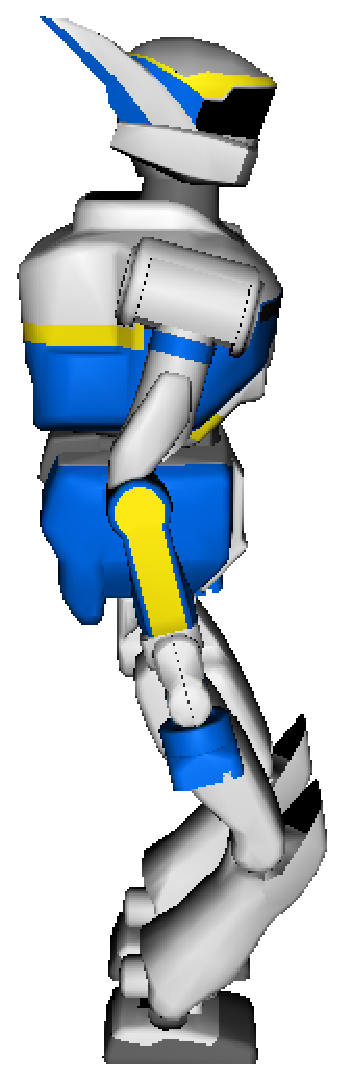
\includegraphics[scale=0.41]{hrp2_side.eps}}
        \subcaption{
            side view
        }
        \label{fig.hrp2_side}
    \end{minipage}
    \hfill
    \begin{minipage}[t]{0.49\textwidth}
        \centering{%
        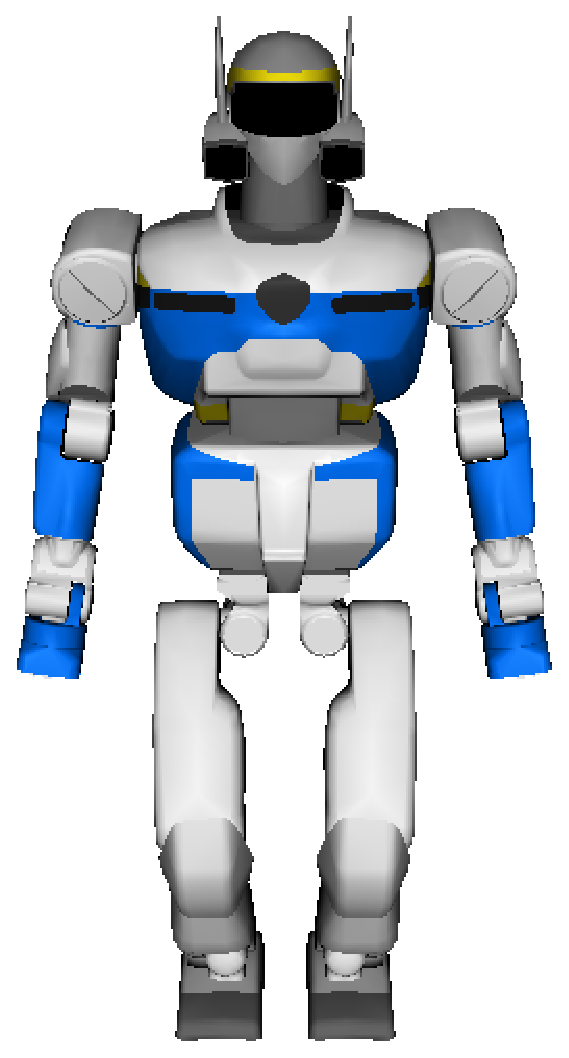
\includegraphics[scale=0.41]{hrp2_front.eps}}
        \subcaption{
            front view
        }
        \label{fig.hrp2_front}
    \end{minipage}
    \caption{
        \sn{HRP-2} robot.
    }
    \label{fig.hrp2}
\end{figure}


Unless stated otherwise, we control and simulate an \sn{HRP-2} robot depicted
in \cref{fig.hrp2} \cite{Kaneko2004icra}. In these cases we assume a perfect
model and perfect inertial measurement unit. The robot has $30$ actuated
joints, its total weight is around $57~[\MT{kg}]$, and the height is around
$1.5~[m]$. The control sampling interval is chosen to be $5~[\MT{ms}]$
($200~[\MT{Hz}]$).



%%%%%%%%%%%%%%%%%%%%%%%%%%%%%%%%%%%%%%%%%%%%%%%%%%%%%%%%%%%%%%%%%%%%%%%%%%%%%%%%
%%%%%%%%%%%%%%%%%%%%%%%%%%%%%%%%%%%%%%%%%%%%%%%%%%%%%%%%%%%%%%%%%%%%%%%%%%%%%%%%
%%%%%%%%%%%%%%%%%%%%%%%%%%%%%%%%%%%%%%%%%%%%%%%%%%%%%%%%%%%%%%%%%%%%%%%%%%%%%%%%
\section{Task-driven walking}\label{sec.task_walk}
\vspace{-1cm}
%
\begin{figure}[!htb]
    \begin{minipage}[t]{0.49\textwidth}
        \centering{
            % Title: glps_renderer figure
% Creator: GL2PS 1.3.8, (C) 1999-2012 C. Geuzaine
% For: Octave
% CreationDate: Mon May  9 19:25:21 2016
\setlength{\unitlength}{0.4pt}
\begin{picture}(0,0)
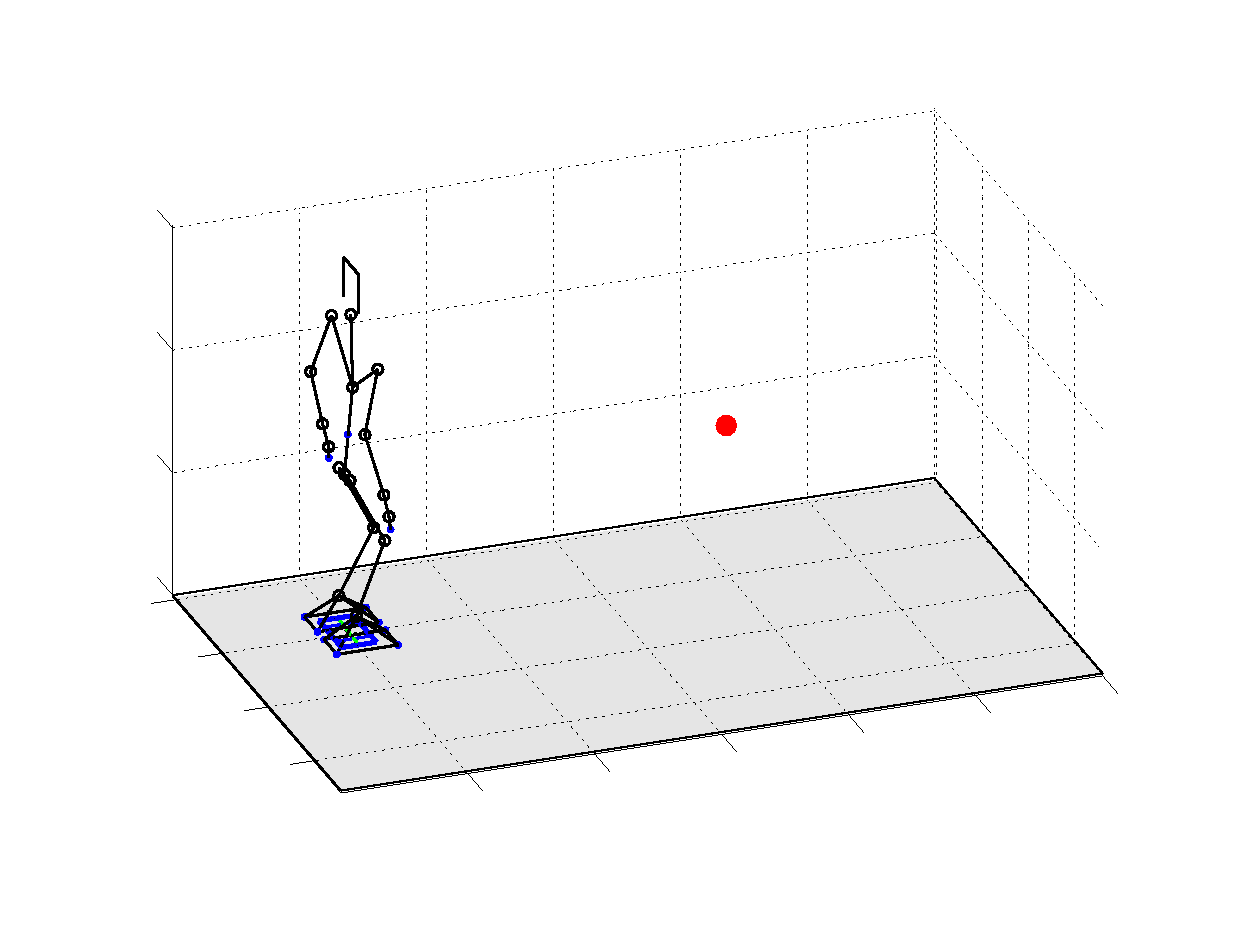
\includegraphics[trim=60  30  50   5,clip,scale=0.4]{test_16_02_robot_1-inc}
\end{picture}%
\begin{picture}(466, 397)(60,30)
\fontsize{7}{0}
\selectfont\put(64.3583,166.387){\makebox(0,0)[br]{\textcolor[rgb]{0,0,0}{{0}}}}
\fontsize{7}{0}
\selectfont\put(64.3583,225.171){\makebox(0,0)[br]{\textcolor[rgb]{0,0,0}{{0.5}}}}
\fontsize{7}{0}
\selectfont\put(64.3583,283.955){\makebox(0,0)[br]{\textcolor[rgb]{0,0,0}{{1}}}}
\fontsize{7}{0}
\selectfont\put(64.3583,342.738){\makebox(0,0)[br]{\textcolor[rgb]{0,0,0}{{1.5}}}}
\fontsize{7}{0}
\selectfont\put(59.8529,149.46){\makebox(0,0)[tr]{\textcolor[rgb]{0,0,0}{{0.5}}}}
\fontsize{7}{0}
\selectfont\put(82.0365,123.702){\makebox(0,0)[tr]{\textcolor[rgb]{0,0,0}{{0}}}}
\fontsize{7}{0}
\selectfont\put(470.853,93.8307){\makebox(0,0)[tl]{\textcolor[rgb]{0,0,0}{{2}}}}
\fontsize{7}{0}
\selectfont\put(531.802,103.206){\makebox(0,0)[tl]{\textcolor[rgb]{0,0,0}{{2.5}}}}
\fontsize{7}{0}
\selectfont\put(104.22,97.9436){\makebox(0,0)[tr]{\textcolor[rgb]{0,0,0}{{-0.5}}}}
\fontsize{7}{0}
\selectfont\put(126.404,72.1854){\makebox(0,0)[tr]{\textcolor[rgb]{0,0,0}{{-1}}}}
\fontsize{7}{0}
\selectfont\put(227.056,56.3298){\makebox(0,0)[tl]{\textcolor[rgb]{0,0,0}{{0}}}}
\fontsize{7}{0}
\selectfont\put(288.005,65.705){\makebox(0,0)[tl]{\textcolor[rgb]{0,0,0}{{0.5}}}}
\fontsize{7}{0}
\selectfont\put(348.954,75.0803){\makebox(0,0)[tl]{\textcolor[rgb]{0,0,0}{{1}}}}
\fontsize{7}{0}
\selectfont\put(409.903,84.4555){\makebox(0,0)[tl]{\textcolor[rgb]{0,0,0}{{1.5}}}}
\end{picture}

            \subcaption{initial}
            \label{fig.task_walk.1}
        }
    \end{minipage}
    \hfill
    \begin{minipage}[t]{0.49\textwidth}
        \centering{
            % Title: glps_renderer figure
% Creator: GL2PS 1.3.8, (C) 1999-2012 C. Geuzaine
% For: Octave
% CreationDate: Mon May  9 19:25:23 2016
\setlength{\unitlength}{0.4pt}
\begin{picture}(0,0)
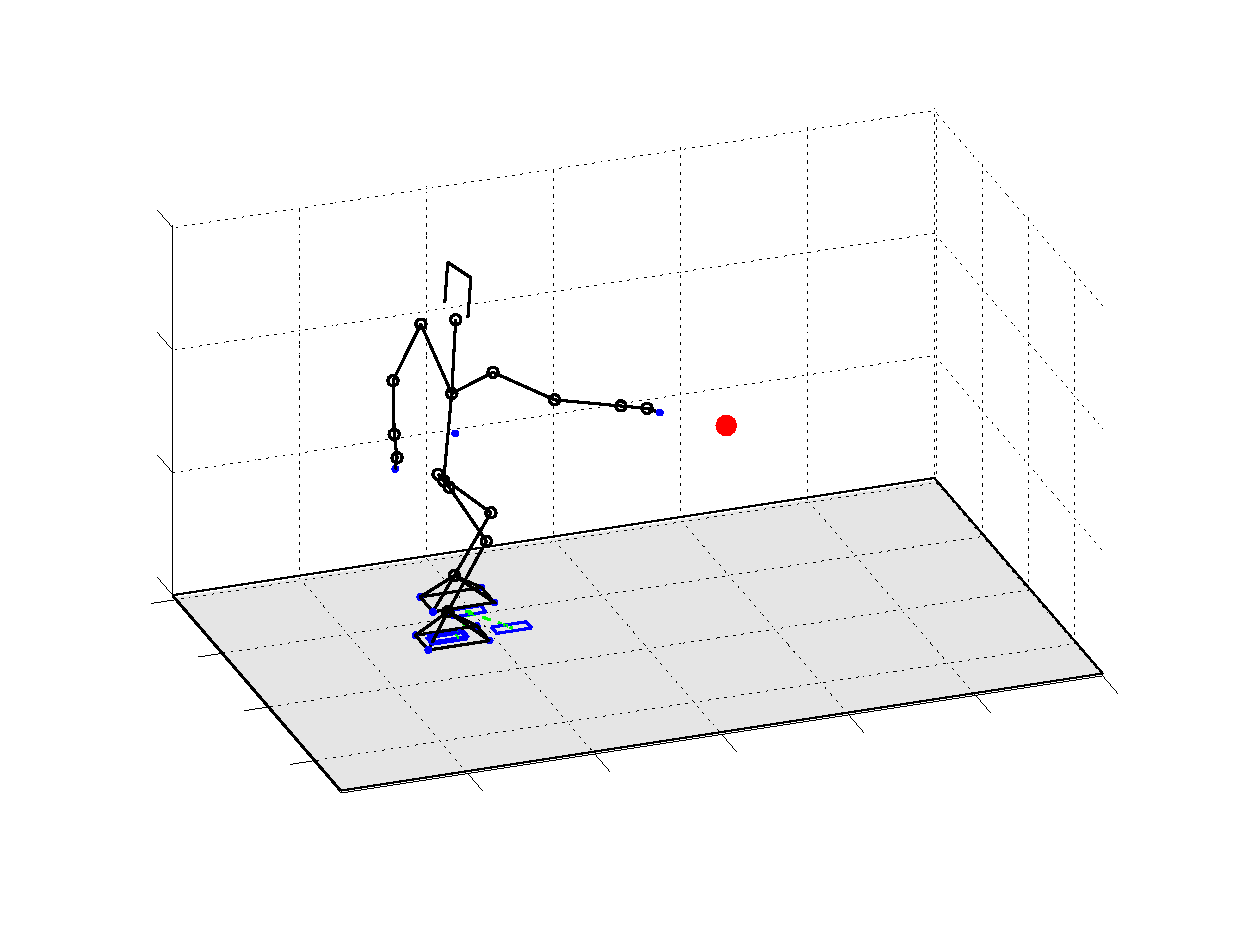
\includegraphics[trim=60  30  50   5,clip,scale=0.4]{test_16_02_robot_501-inc}
\end{picture}%
\begin{picture}(466, 397)(60,30)
\fontsize{7}{0}
\selectfont\put(64.3583,166.387){\makebox(0,0)[br]{\textcolor[rgb]{0,0,0}{{0}}}}
\fontsize{7}{0}
\selectfont\put(64.3583,225.171){\makebox(0,0)[br]{\textcolor[rgb]{0,0,0}{{0.5}}}}
\fontsize{7}{0}
\selectfont\put(64.3583,283.955){\makebox(0,0)[br]{\textcolor[rgb]{0,0,0}{{1}}}}
\fontsize{7}{0}
\selectfont\put(64.3583,342.738){\makebox(0,0)[br]{\textcolor[rgb]{0,0,0}{{1.5}}}}
\fontsize{7}{0}
\selectfont\put(59.8529,149.46){\makebox(0,0)[tr]{\textcolor[rgb]{0,0,0}{{0.5}}}}
\fontsize{7}{0}
\selectfont\put(82.0365,123.702){\makebox(0,0)[tr]{\textcolor[rgb]{0,0,0}{{0}}}}
\fontsize{7}{0}
\selectfont\put(470.853,93.8307){\makebox(0,0)[tl]{\textcolor[rgb]{0,0,0}{{2}}}}
\fontsize{7}{0}
\selectfont\put(531.802,103.206){\makebox(0,0)[tl]{\textcolor[rgb]{0,0,0}{{2.5}}}}
\fontsize{7}{0}
\selectfont\put(104.22,97.9436){\makebox(0,0)[tr]{\textcolor[rgb]{0,0,0}{{-0.5}}}}
\fontsize{7}{0}
\selectfont\put(126.404,72.1854){\makebox(0,0)[tr]{\textcolor[rgb]{0,0,0}{{-1}}}}
\fontsize{7}{0}
\selectfont\put(227.056,56.3298){\makebox(0,0)[tl]{\textcolor[rgb]{0,0,0}{{0}}}}
\fontsize{7}{0}
\selectfont\put(288.005,65.705){\makebox(0,0)[tl]{\textcolor[rgb]{0,0,0}{{0.5}}}}
\fontsize{7}{0}
\selectfont\put(348.954,75.0803){\makebox(0,0)[tl]{\textcolor[rgb]{0,0,0}{{1}}}}
\fontsize{7}{0}
\selectfont\put(409.903,84.4555){\makebox(0,0)[tl]{\textcolor[rgb]{0,0,0}{{1.5}}}}
\end{picture}

            \subcaption{after $2.5$ seconds}
            \label{fig.task_walk.2}
        }
    \end{minipage}
    \begin{minipage}[t]{0.49\textwidth}
        \centering{
            % Title: glps_renderer figure
% Creator: GL2PS 1.3.8, (C) 1999-2012 C. Geuzaine
% For: Octave
% CreationDate: Mon May  9 19:25:24 2016
\setlength{\unitlength}{0.4pt}
\begin{picture}(0,0)
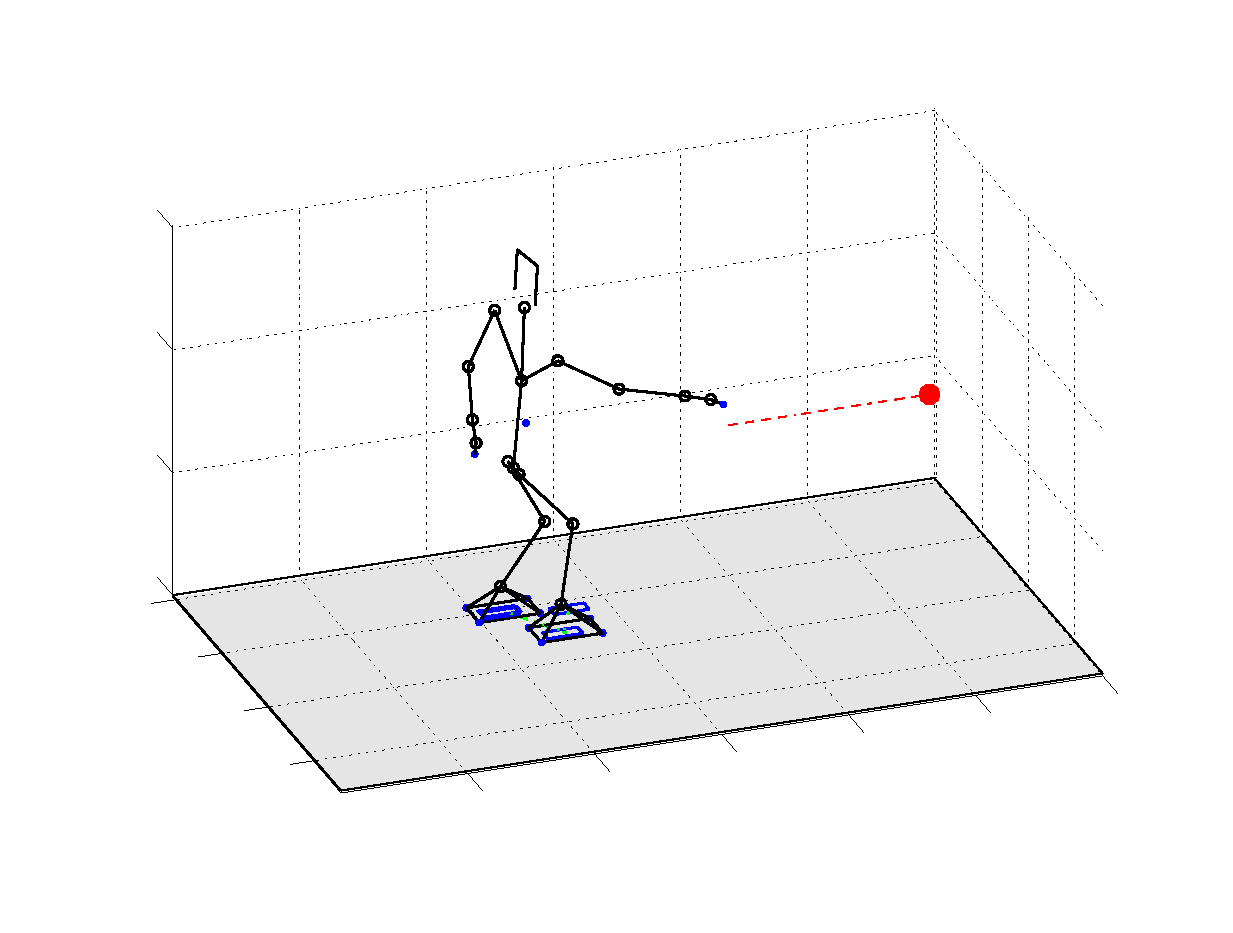
\includegraphics[trim=60  30  50   5,clip,scale=0.4]{test_16_02_robot_1001-inc}
\end{picture}%
\begin{picture}(466, 397)(60,30)
\fontsize{7}{0}
\selectfont\put(64.3583,166.387){\makebox(0,0)[br]{\textcolor[rgb]{0,0,0}{{0}}}}
\fontsize{7}{0}
\selectfont\put(64.3583,225.171){\makebox(0,0)[br]{\textcolor[rgb]{0,0,0}{{0.5}}}}
\fontsize{7}{0}
\selectfont\put(64.3583,283.955){\makebox(0,0)[br]{\textcolor[rgb]{0,0,0}{{1}}}}
\fontsize{7}{0}
\selectfont\put(64.3583,342.738){\makebox(0,0)[br]{\textcolor[rgb]{0,0,0}{{1.5}}}}
\fontsize{7}{0}
\selectfont\put(59.8529,149.46){\makebox(0,0)[tr]{\textcolor[rgb]{0,0,0}{{0.5}}}}
\fontsize{7}{0}
\selectfont\put(82.0365,123.702){\makebox(0,0)[tr]{\textcolor[rgb]{0,0,0}{{0}}}}
\fontsize{7}{0}
\selectfont\put(531.802,103.206){\makebox(0,0)[tl]{\textcolor[rgb]{0,0,0}{{2.5}}}}
\fontsize{7}{0}
\selectfont\put(104.22,97.9436){\makebox(0,0)[tr]{\textcolor[rgb]{0,0,0}{{-0.5}}}}
\fontsize{7}{0}
\selectfont\put(126.404,72.1854){\makebox(0,0)[tr]{\textcolor[rgb]{0,0,0}{{-1}}}}
\fontsize{7}{0}
\selectfont\put(227.056,56.3298){\makebox(0,0)[tl]{\textcolor[rgb]{0,0,0}{{0}}}}
\fontsize{7}{0}
\selectfont\put(288.005,65.705){\makebox(0,0)[tl]{\textcolor[rgb]{0,0,0}{{0.5}}}}
\fontsize{7}{0}
\selectfont\put(348.954,75.0803){\makebox(0,0)[tl]{\textcolor[rgb]{0,0,0}{{1}}}}
\fontsize{7}{0}
\selectfont\put(409.903,84.4555){\makebox(0,0)[tl]{\textcolor[rgb]{0,0,0}{{1.5}}}}
\fontsize{7}{0}
\selectfont\put(470.853,93.8307){\makebox(0,0)[tl]{\textcolor[rgb]{0,0,0}{{2}}}}
\end{picture}

            \subcaption{after $5$ seconds}
            \label{fig.task_walk.3}
        }
    \end{minipage}
    \hfill
    \begin{minipage}[t]{0.49\textwidth}
        \centering{
            % Title: glps_renderer figure
% Creator: GL2PS 1.3.8, (C) 1999-2012 C. Geuzaine
% For: Octave
% CreationDate: Mon May  9 19:25:25 2016
\setlength{\unitlength}{0.4pt}
\begin{picture}(0,0)
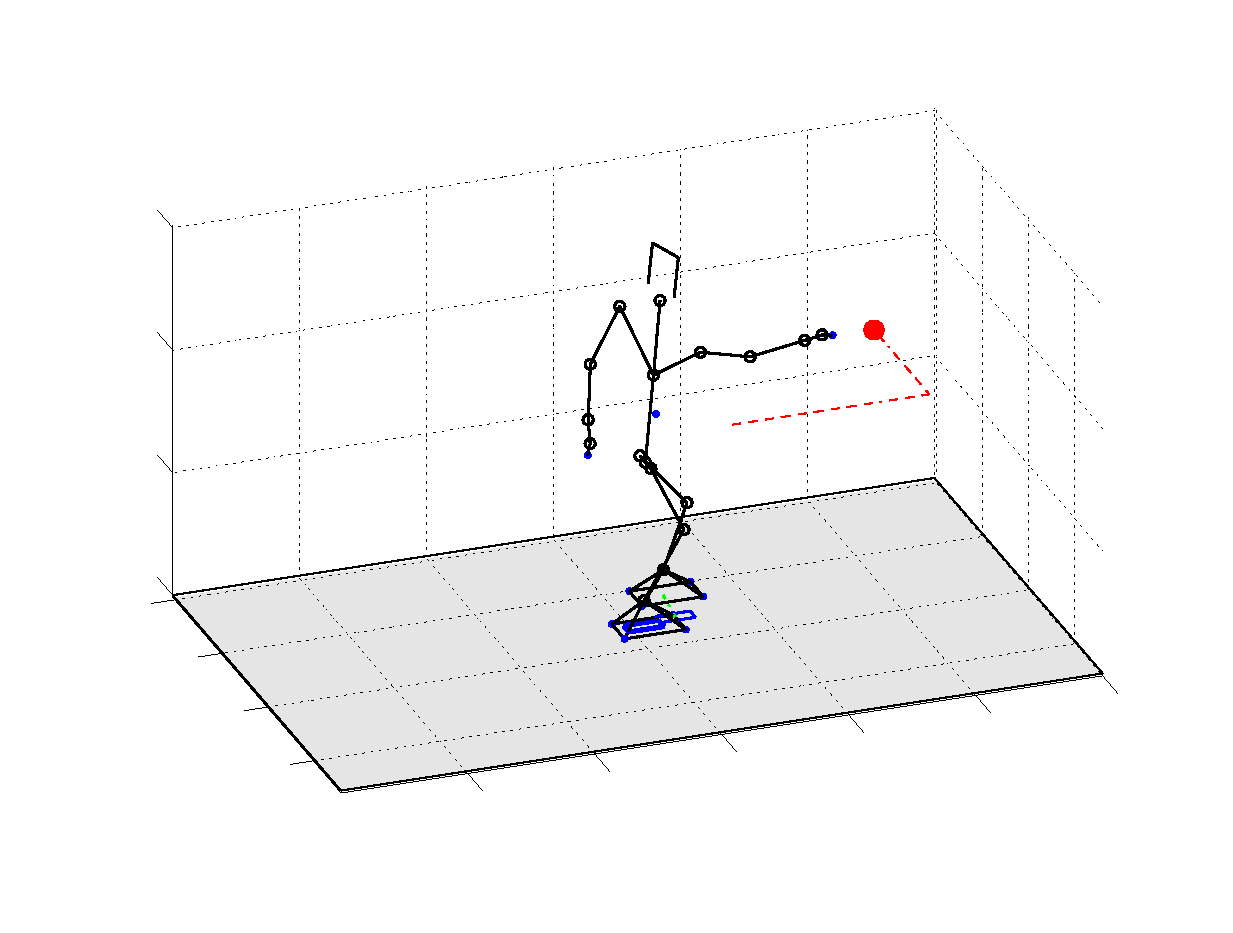
\includegraphics[trim=60  30  50   5,clip,scale=0.4]{test_16_02_robot_1501-inc}
\end{picture}%
\begin{picture}(466, 397)(60,30)
\fontsize{7}{0}
\selectfont\put(64.3583,166.387){\makebox(0,0)[br]{\textcolor[rgb]{0,0,0}{{0}}}}
\fontsize{7}{0}
\selectfont\put(64.3583,225.171){\makebox(0,0)[br]{\textcolor[rgb]{0,0,0}{{0.5}}}}
\fontsize{7}{0}
\selectfont\put(64.3583,283.955){\makebox(0,0)[br]{\textcolor[rgb]{0,0,0}{{1}}}}
\fontsize{7}{0}
\selectfont\put(64.3583,342.738){\makebox(0,0)[br]{\textcolor[rgb]{0,0,0}{{1.5}}}}
\fontsize{7}{0}
\selectfont\put(59.8529,149.46){\makebox(0,0)[tr]{\textcolor[rgb]{0,0,0}{{0.5}}}}
\fontsize{7}{0}
\selectfont\put(82.0365,123.702){\makebox(0,0)[tr]{\textcolor[rgb]{0,0,0}{{0}}}}
\fontsize{7}{0}
\selectfont\put(126.404,72.1854){\makebox(0,0)[tr]{\textcolor[rgb]{0,0,0}{{-1}}}}
\fontsize{7}{0}
\selectfont\put(104.22,97.9436){\makebox(0,0)[tr]{\textcolor[rgb]{0,0,0}{{-0.5}}}}
\fontsize{7}{0}
\selectfont\put(227.056,56.3298){\makebox(0,0)[tl]{\textcolor[rgb]{0,0,0}{{0}}}}
\fontsize{7}{0}
\selectfont\put(288.005,65.705){\makebox(0,0)[tl]{\textcolor[rgb]{0,0,0}{{0.5}}}}
\fontsize{7}{0}
\selectfont\put(348.954,75.0803){\makebox(0,0)[tl]{\textcolor[rgb]{0,0,0}{{1}}}}
\fontsize{7}{0}
\selectfont\put(409.903,84.4555){\makebox(0,0)[tl]{\textcolor[rgb]{0,0,0}{{1.5}}}}
\fontsize{7}{0}
\selectfont\put(470.853,93.8307){\makebox(0,0)[tl]{\textcolor[rgb]{0,0,0}{{2}}}}
\fontsize{7}{0}
\selectfont\put(531.802,103.206){\makebox(0,0)[tl]{\textcolor[rgb]{0,0,0}{{2.5}}}}
\end{picture}

            \subcaption{after $7.5$ seconds}
            \label{fig.task_walk.4}
        }
    \end{minipage}
    \begin{minipage}[t]{0.49\textwidth}
        \centering{
            % Title: glps_renderer figure
% Creator: GL2PS 1.3.8, (C) 1999-2012 C. Geuzaine
% For: Octave
% CreationDate: Mon May  9 19:25:26 2016
\setlength{\unitlength}{0.4pt}
\begin{picture}(0,0)
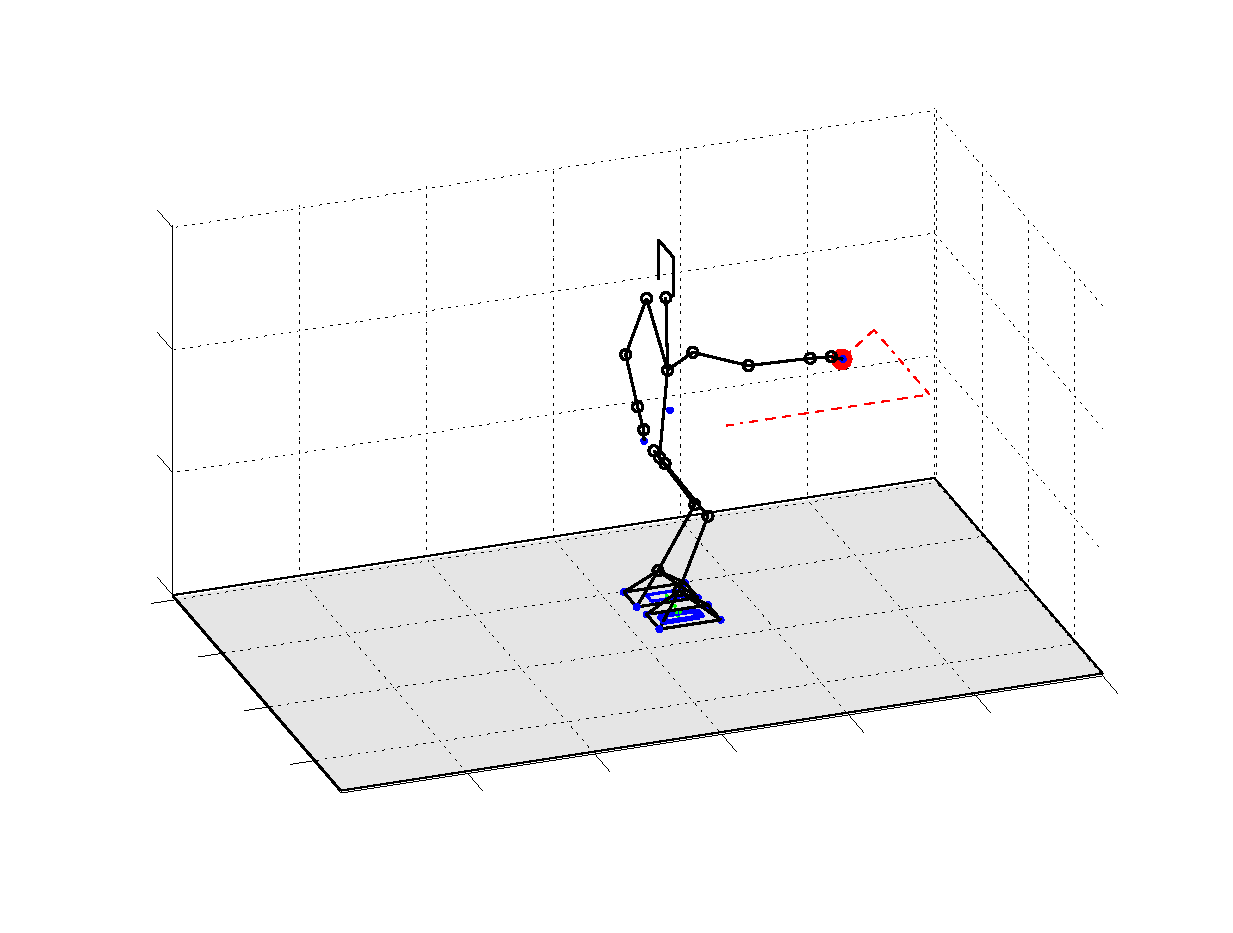
\includegraphics[trim=60  30  50   5,clip,scale=0.4]{test_16_02_robot_2001-inc}
\end{picture}%
\begin{picture}(466, 397)(60,30)
\fontsize{7}{0}
\selectfont\put(64.3583,166.387){\makebox(0,0)[br]{\textcolor[rgb]{0,0,0}{{0}}}}
\fontsize{7}{0}
\selectfont\put(64.3583,225.171){\makebox(0,0)[br]{\textcolor[rgb]{0,0,0}{{0.5}}}}
\fontsize{7}{0}
\selectfont\put(64.3583,283.955){\makebox(0,0)[br]{\textcolor[rgb]{0,0,0}{{1}}}}
\fontsize{7}{0}
\selectfont\put(64.3583,342.738){\makebox(0,0)[br]{\textcolor[rgb]{0,0,0}{{1.5}}}}
\fontsize{7}{0}
\selectfont\put(59.8529,149.46){\makebox(0,0)[tr]{\textcolor[rgb]{0,0,0}{{0.5}}}}
\fontsize{7}{0}
\selectfont\put(82.0365,123.702){\makebox(0,0)[tr]{\textcolor[rgb]{0,0,0}{{0}}}}
\fontsize{7}{0}
\selectfont\put(227.056,56.3298){\makebox(0,0)[tl]{\textcolor[rgb]{0,0,0}{{0}}}}
\fontsize{7}{0}
\selectfont\put(288.005,65.705){\makebox(0,0)[tl]{\textcolor[rgb]{0,0,0}{{0.5}}}}
\fontsize{7}{0}
\selectfont\put(348.954,75.0803){\makebox(0,0)[tl]{\textcolor[rgb]{0,0,0}{{1}}}}
\fontsize{7}{0}
\selectfont\put(409.903,84.4555){\makebox(0,0)[tl]{\textcolor[rgb]{0,0,0}{{1.5}}}}
\fontsize{7}{0}
\selectfont\put(470.853,93.8307){\makebox(0,0)[tl]{\textcolor[rgb]{0,0,0}{{2}}}}
\fontsize{7}{0}
\selectfont\put(531.802,103.206){\makebox(0,0)[tl]{\textcolor[rgb]{0,0,0}{{2.5}}}}
\fontsize{7}{0}
\selectfont\put(126.404,72.1854){\makebox(0,0)[tr]{\textcolor[rgb]{0,0,0}{{-1}}}}
\fontsize{7}{0}
\selectfont\put(104.22,97.9436){\makebox(0,0)[tr]{\textcolor[rgb]{0,0,0}{{-0.5}}}}
\end{picture}

            \subcaption{after $10$ seconds}
            \label{fig.task_walk.5}
        }
    \end{minipage}
    \hfill
    \begin{minipage}[t]{0.49\textwidth}
        \centering{
            % Title: glps_renderer figure
% Creator: GL2PS 1.3.8, (C) 1999-2012 C. Geuzaine
% For: Octave
% CreationDate: Mon May  9 19:25:27 2016
\setlength{\unitlength}{0.4pt}
\begin{picture}(0,0)
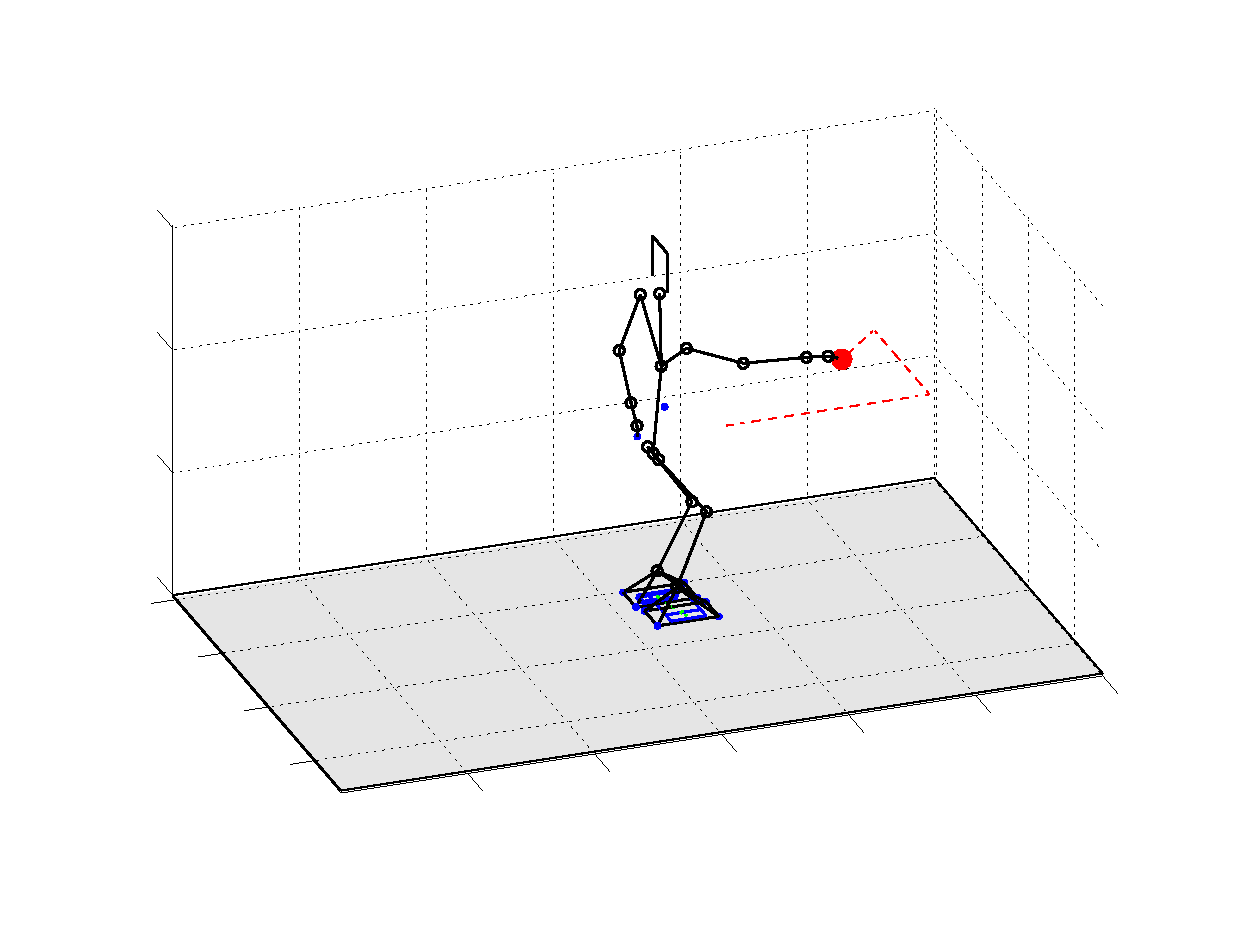
\includegraphics[trim=60  30  50   5,clip,scale=0.4]{test_16_02_robot_2501-inc}
\end{picture}%
\begin{picture}(466, 397)(60,30)
\fontsize{7}{0}
\selectfont\put(64.3583,166.387){\makebox(0,0)[br]{\textcolor[rgb]{0,0,0}{{0}}}}
\fontsize{7}{0}
\selectfont\put(64.3583,225.171){\makebox(0,0)[br]{\textcolor[rgb]{0,0,0}{{0.5}}}}
\fontsize{7}{0}
\selectfont\put(64.3583,283.955){\makebox(0,0)[br]{\textcolor[rgb]{0,0,0}{{1}}}}
\fontsize{7}{0}
\selectfont\put(64.3583,342.738){\makebox(0,0)[br]{\textcolor[rgb]{0,0,0}{{1.5}}}}
\fontsize{7}{0}
\selectfont\put(59.8529,149.46){\makebox(0,0)[tr]{\textcolor[rgb]{0,0,0}{{0.5}}}}
\fontsize{7}{0}
\selectfont\put(82.0365,123.702){\makebox(0,0)[tr]{\textcolor[rgb]{0,0,0}{{0}}}}
\fontsize{7}{0}
\selectfont\put(227.056,56.3298){\makebox(0,0)[tl]{\textcolor[rgb]{0,0,0}{{0}}}}
\fontsize{7}{0}
\selectfont\put(288.005,65.705){\makebox(0,0)[tl]{\textcolor[rgb]{0,0,0}{{0.5}}}}
\fontsize{7}{0}
\selectfont\put(348.954,75.0803){\makebox(0,0)[tl]{\textcolor[rgb]{0,0,0}{{1}}}}
\fontsize{7}{0}
\selectfont\put(409.903,84.4555){\makebox(0,0)[tl]{\textcolor[rgb]{0,0,0}{{1.5}}}}
\fontsize{7}{0}
\selectfont\put(470.853,93.8307){\makebox(0,0)[tl]{\textcolor[rgb]{0,0,0}{{2}}}}
\fontsize{7}{0}
\selectfont\put(531.802,103.206){\makebox(0,0)[tl]{\textcolor[rgb]{0,0,0}{{2.5}}}}
\fontsize{7}{0}
\selectfont\put(126.404,72.1854){\makebox(0,0)[tr]{\textcolor[rgb]{0,0,0}{{-1}}}}
\fontsize{7}{0}
\selectfont\put(104.22,97.9436){\makebox(0,0)[tr]{\textcolor[rgb]{0,0,0}{{-0.5}}}}
\end{picture}

            \subcaption{after $12.5$ seconds}
            \label{fig.task_walk.6}
        }
    \end{minipage}
    \caption[Task-driven walk: configurations of the robot during the simulation.]{
        Task-driven walk: configurations of the robot during the simulation.
        Red point indicates position of the target, blue rectangles -- current
        and anticipated positions of the feet.
    }
    \label{fig.task_walk}
\end{figure}
%

It is typical to express high level goals of humanoid robot control using whole
body tasks, execution of which may require locomotion. For example, it might be
necessary to approach an object before grasping it. In such situations it is
necessary to anticipate walking motions taking the whole body tasks into
account. This, however, may not be straightforward when anticipation with an
approximate model is performed, due to simplifications made during the
construction of the model (see \cref{sec.mmpc}). For example, in the case of
point-mass models it is common to map whole body tasks to motions of the
\ac{CoM} or feet \cite{Yoshida2006humanoids, Nishiwaki2003icra,
Fukumoto2004iros, Herdt2010auro}. Such mappings, however, are often task- and
model- specific and their development requires human involvement. \acf{MMPC}
addresses this problem by mixing approximate and whole body models to allow
their automatic interaction without any additional mapping procedures. It also
allows to account for multiple tasks simultaneously in a straightforward way.

%
\begin{figure}[!htb]
    \begin{minipage}[t]{\textwidth}
        \centering{
            % Title: glps_renderer figure
% Creator: GL2PS 1.3.8, (C) 1999-2012 C. Geuzaine
% For: Octave
% CreationDate: Wed Mar 23 18:52:37 2016
\setlength{\unitlength}{0.8pt}
\begin{picture}(0,0)
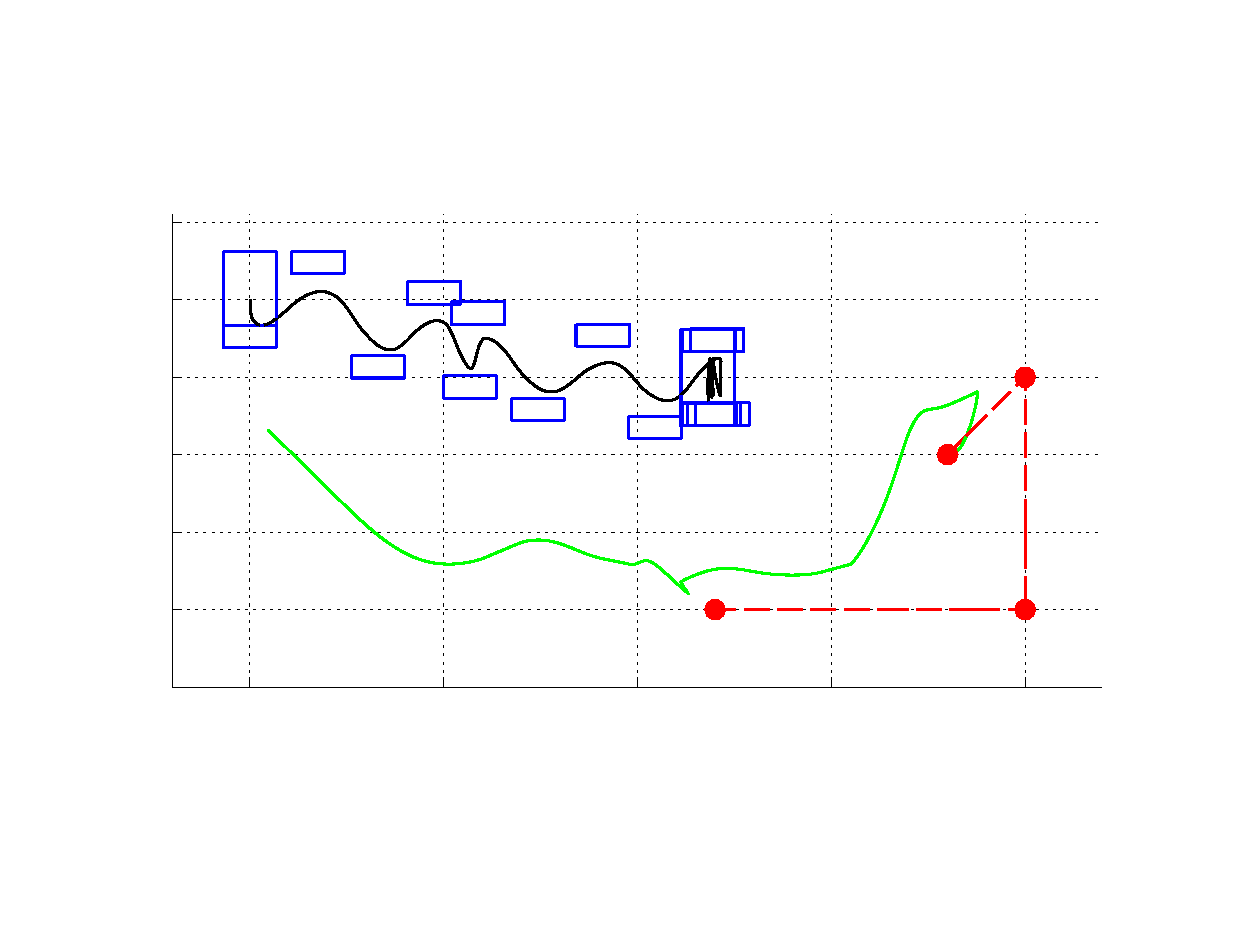
\includegraphics[trim=50  75  50  90,clip,scale=0.8]{steps_16_02_03_N16_nodist-inc}
\end{picture}%
\begin{picture}(476, 267)(50,75)
\fontsize{11}{0}
\selectfont\put(111.96,104.974){\makebox(0,0)[t]{\textcolor[rgb]{0,0,0}{{0}}}}
\fontsize{11}{0}
\selectfont\put(204.987,104.974){\makebox(0,0)[t]{\textcolor[rgb]{0,0,0}{{0.5}}}}
\fontsize{11}{0}
\selectfont\put(298.015,104.974){\makebox(0,0)[t]{\textcolor[rgb]{0,0,0}{{1}}}}
\fontsize{11}{0}
\selectfont\put(391.042,104.974){\makebox(0,0)[t]{\textcolor[rgb]{0,0,0}{{1.5}}}}
\fontsize{11}{0}
\selectfont\put(484.069,104.974){\makebox(0,0)[t]{\textcolor[rgb]{0,0,0}{{2}}}}
\fontsize{11}{0}
\selectfont\put(69.8755,109.977){\makebox(0,0)[r]{\textcolor[rgb]{0,0,0}{{-1}}}}
\fontsize{11}{0}
\selectfont\put(69.8755,147.188){\makebox(0,0)[r]{\textcolor[rgb]{0,0,0}{{-0.8}}}}
\fontsize{11}{0}
\selectfont\put(69.8755,184.399){\makebox(0,0)[r]{\textcolor[rgb]{0,0,0}{{-0.6}}}}
\fontsize{11}{0}
\selectfont\put(69.8755,221.61){\makebox(0,0)[r]{\textcolor[rgb]{0,0,0}{{-0.4}}}}
\fontsize{11}{0}
\selectfont\put(69.8755,258.821){\makebox(0,0)[r]{\textcolor[rgb]{0,0,0}{{-0.2}}}}
\fontsize{11}{0}
\selectfont\put(69.8755,296.032){\makebox(0,0)[r]{\textcolor[rgb]{0,0,0}{{0}}}}
\fontsize{11}{0}
\selectfont\put(69.8755,333.243){\makebox(0,0)[r]{\textcolor[rgb]{0,0,0}{{0.2}}}}
\fontsize{11}{0}
\selectfont\put(298.08,88.9738){\makebox(0,0)[t]{\textcolor[rgb]{0,0,0}{{$x~[m]$}}}}
\fontsize{11}{0}
\selectfont\put(40.8755,223.56){\rotatebox{90}{\makebox(0,0)[b]{\textcolor[rgb]{0,0,0}{{$y~[m]$}}}}}
\fontsize{11}{0}
\selectfont\put(344.528,137.886){\makebox(0,0)[l]{\textcolor[rgb]{0,0,0}{{1}}}}
\fontsize{11}{0}
\selectfont\put(493.372,137.886){\makebox(0,0)[l]{\textcolor[rgb]{0,0,0}{{2}}}}
\fontsize{11}{0}
\selectfont\put(493.372,249.518){\makebox(0,0)[l]{\textcolor[rgb]{0,0,0}{{3}}}}
\fontsize{11}{0}
\selectfont\put(456.161,212.307){\makebox(0,0)[l]{\textcolor[rgb]{0,0,0}{{4}}}}
\end{picture}

            \subcaption{without disturbances}
            \label{fig.task_walk_steps.nodist}
        }
    \end{minipage}
    \begin{minipage}[t]{\textwidth}
        \centering{
            % Title: glps_renderer figure
% Creator: GL2PS 1.3.8, (C) 1999-2012 C. Geuzaine
% For: Octave
% CreationDate: Wed Mar 23 18:52:34 2016
\setlength{\unitlength}{0.8pt}
\begin{picture}(0,0)
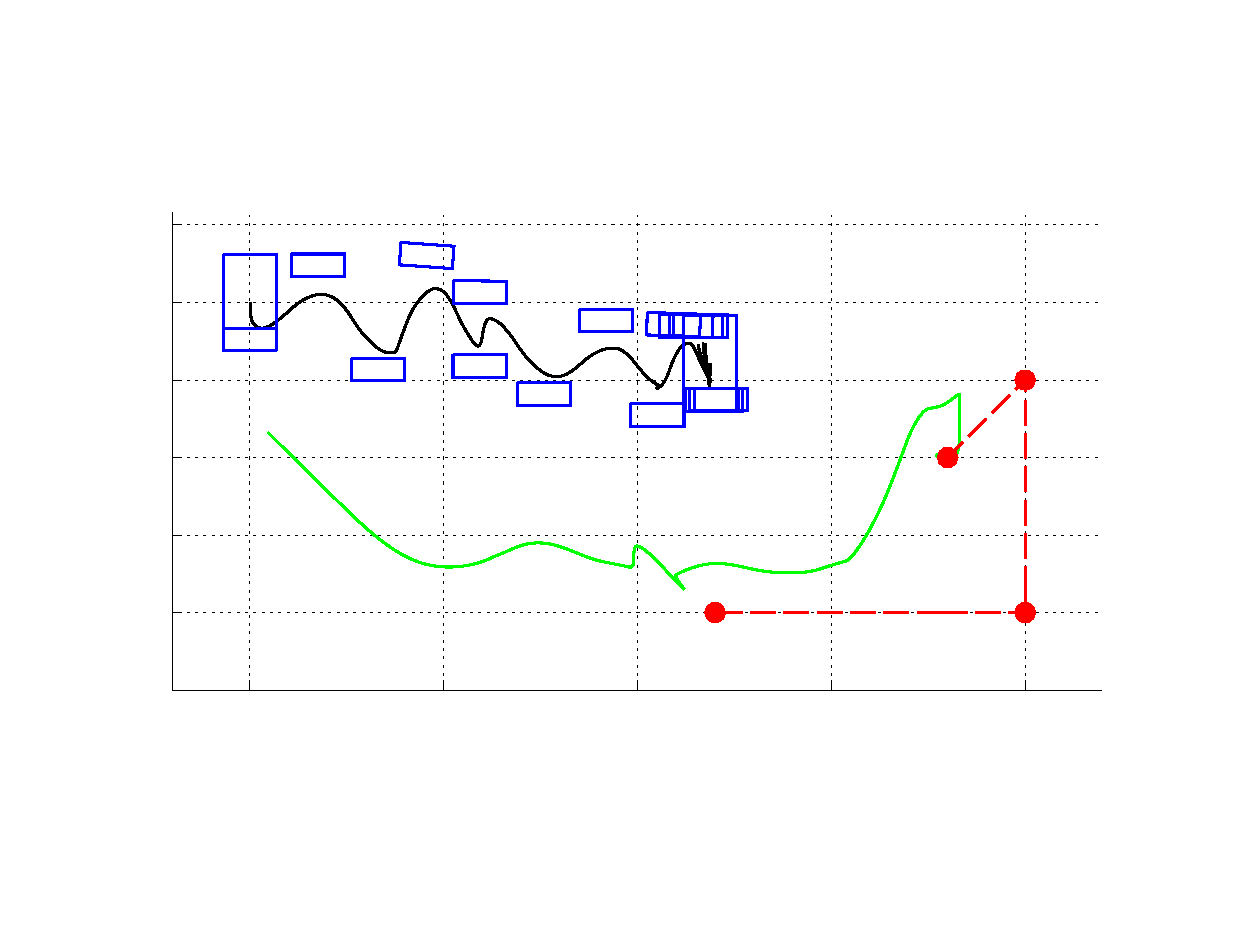
\includegraphics[trim=50  75  50  90,clip,scale=0.8]{steps_16_02_01_N16-inc}
\end{picture}%
\begin{picture}(476, 267)(50,75)
\fontsize{11}{0}
\selectfont\put(111.96,103.583){\makebox(0,0)[t]{\textcolor[rgb]{0,0,0}{{0}}}}
\fontsize{11}{0}
\selectfont\put(204.987,103.583){\makebox(0,0)[t]{\textcolor[rgb]{0,0,0}{{0.5}}}}
\fontsize{11}{0}
\selectfont\put(298.015,103.583){\makebox(0,0)[t]{\textcolor[rgb]{0,0,0}{{1}}}}
\fontsize{11}{0}
\selectfont\put(391.042,103.583){\makebox(0,0)[t]{\textcolor[rgb]{0,0,0}{{1.5}}}}
\fontsize{11}{0}
\selectfont\put(484.069,103.583){\makebox(0,0)[t]{\textcolor[rgb]{0,0,0}{{2}}}}
\fontsize{11}{0}
\selectfont\put(69.8755,108.582){\makebox(0,0)[r]{\textcolor[rgb]{0,0,0}{{-1}}}}
\fontsize{11}{0}
\selectfont\put(69.8755,145.793){\makebox(0,0)[r]{\textcolor[rgb]{0,0,0}{{-0.8}}}}
\fontsize{11}{0}
\selectfont\put(69.8755,183.004){\makebox(0,0)[r]{\textcolor[rgb]{0,0,0}{{-0.6}}}}
\fontsize{11}{0}
\selectfont\put(69.8755,220.215){\makebox(0,0)[r]{\textcolor[rgb]{0,0,0}{{-0.4}}}}
\fontsize{11}{0}
\selectfont\put(69.8755,257.425){\makebox(0,0)[r]{\textcolor[rgb]{0,0,0}{{-0.2}}}}
\fontsize{11}{0}
\selectfont\put(69.8755,294.636){\makebox(0,0)[r]{\textcolor[rgb]{0,0,0}{{0}}}}
\fontsize{11}{0}
\selectfont\put(69.8755,331.847){\makebox(0,0)[r]{\textcolor[rgb]{0,0,0}{{0.2}}}}
\fontsize{11}{0}
\selectfont\put(298.08,87.5828){\makebox(0,0)[t]{\textcolor[rgb]{0,0,0}{{$x~[m]$}}}}
\fontsize{11}{0}
\selectfont\put(40.8755,223.56){\rotatebox{90}{\makebox(0,0)[b]{\textcolor[rgb]{0,0,0}{{$y~[m]$}}}}}
\fontsize{11}{0}
\selectfont\put(344.528,136.49){\makebox(0,0)[l]{\textcolor[rgb]{0,0,0}{{1}}}}
\fontsize{11}{0}
\selectfont\put(493.372,136.49){\makebox(0,0)[l]{\textcolor[rgb]{0,0,0}{{2}}}}
\fontsize{11}{0}
\selectfont\put(493.372,248.123){\makebox(0,0)[l]{\textcolor[rgb]{0,0,0}{{3}}}}
\fontsize{11}{0}
\selectfont\put(456.161,210.912){\makebox(0,0)[l]{\textcolor[rgb]{0,0,0}{{4}}}}
\end{picture}

            \subcaption{with disturbances}
            \label{fig.task_walk_steps.dist}
        }
    \end{minipage}
    \caption[Task-driven walk: top view.]{
        Task-driven walk: top view. Footsteps are represented by rectangles,
        trajectory of the \ac{CoM} is in black, trajectory of the hand is in
        green, while the trajectory of the target is in dashed red. Numbers
        indicate ordering of the target positions.
    }
    \label{fig.task_walk_steps}
\end{figure}
%

The interplay between the models in \ac{MMPC} was shown in
\cite{Sherikov2014humanoids}, where a whole body task induces walking motion.
The task is to reach a varying target point with the right hand of the robot
(see \cref{fig.task_walk,fig.task_walk_steps}). We also demonstrated that this
controller performs automatic repositioning of the feet in order to compensate
for disturbances applied to the robot. We describe this controller and
simulation setting in \cref{sec.task_walk_controller,sec.task_walk_setting}.
The obtained results are discussed in \cref{sec.task_walk_results}.




%%%%%%%%%%%%%%%%%%%%%%%%%%%%%%%%%%%%%%%%%%%%%%%%%%%%%%%%%%%%%%%%%%%%%%%%%%%%%%%%
\subsection{Setting}\label{sec.task_walk_setting}

We evaluate the proposed controller in a simulation, which lasts for
approximately $15$ second. During this time the robot has to reach a target
with its right hand. Initially, the target cannot be reached by the robot while
standing. During the simulation the target is repositioned at $4.6$, $6.25$,
and $8$ second in an unpredictable way (see \cref{fig.task_walk_steps}). In
order to further complicate the task for the controller, we apply disturbances
to the robot at $2.5$ second from the right ($\impulseC_d^y = 15~[\MT{Ns}]$)
and at $7$ second from the front ($\impulseC_d^x = -15~[\MT{Ns}]$). The
disturbances are simulated as described in \cref{app.collision}.


Thus, the goal of the controller is to automatically choose positions of the
feet on the ground in order to reach the target and compensate for
disturbances.



%%%%%%%%%%%%%%%%%%%%%%%%%%%%%%%%%%%%%%%%%%%%%%%%%%%%%%%%%%%%%%%%%%%%%%%%%%%%%%%%
\subsection{Design of the controller}\label{sec.task_walk_controller}


We construct a hierarchy corresponding to \ac{MMPC} controller based on the
whole body (\nameref{model.WB}) and point-mass (\nameref{model.PPMZ}) models as
proposed in \cref{sec.mmpc_hierarchy}. In order to reduce the size of the
\ac{PLLS} problem, we condense \nameref{model.PPMZ} and eliminate torques from
\nameref{model.WB} in advance (see \cref{sec.plls_preprocessing}). This results
in the following hierarchy:
%
\changeHierarchyStyle{breakable,width=14.5cm,before=\par\smallskip\centering,after=\par}{\setlength{\itemsep}{5pt}}
\begin{hierarchy}[hr.mmpc_walk]
    \level Simple bounds
            \begin{itemize}%[topsep=3pt]
                \item \makebox[5.2cm][l]{
                        $\displaystyle \ubar{\ddq}^{\prime}  \le  \ddqn  \le  \bar{\ddq}^{\prime}$
                    }
                    $30$ joint limits
                \item \makebox[5.2cm][l]{
                        $\displaystyle \V{\lambda}_i \ge \V{0}$
                    }
                    $3 M$ constraints due to friction cones
                \item \makebox[5.2cm][l]{
                        $\displaystyle \ubarV{\objb}_{\contact,j} \le \Delta\hat{\contact}_{j} \le \barV{\objb}_{\contact,j}$
                    }
                    $2 K$ constraints on foot positions
                \item \makebox[5.2cm][l]{
                        $\displaystyle \ubar{\cop} \le \hat{\cop}_{k+1} \le \bar{\cop}$
                    }
                    $2 N$ constraints on the \acs{CoP} positions
            \end{itemize}

    \level Tasks of the whole body motion controller
            \begin{itemize}%[topsep=3pt]
                \item
                    $\displaystyle
                        \begin{bmatrix}
                            \M{H}_2\\
                            \M{H}_3\\
                        \end{bmatrix}
                        \ddq
                        +
                        \begin{bmatrix}
                            \V{h}_2\\
                            \V{h}_3
                        \end{bmatrix}
                        =
                        m
                        \begin{bmatrix}
                            \T{\Jcom[,2]}\\
                            \T{\Jcom[,3]}
                        \end{bmatrix}
                        \V{g}
                        +
                        \sum_{i=1}^M
                            \begin{bmatrix}
                                \T{\M{J}_{i,2}}\\
                                \T{\M{J}_{i,3}}
                            \end{bmatrix}
                        \begin{bmatrix}
                            \M{V}_i \V{\lambda}_i\\
                            \moment_i
                        \end{bmatrix}
                    $\\[1mm]
                    \makebox[5.2cm][l]{} $6$ equalities due to Newton-Euler equations

                \item
                    $\displaystyle
                    \ubar{\torques}
                    \le
                    \M{H}_1 \ddq  +  \V{h}_1  -  m \T{\Jcom[,1]} \V{g}  -  \sum_{i=1}^M \T{\M{J}_{i,1}}
                    \begin{bmatrix}
                        \M{V}_i \V{\lambda}_i\\
                        \moment_i
                    \end{bmatrix}
                    \le
                    \bar{\torques}
                    $\\[1mm]
                    \makebox[5.2cm][l]{} $30$ bounds on the joint torques

                \item
                    \makebox[5.2cm][l]{
                        $\displaystyle \M{J}_i \ddq + \dotM{J}_i \dq = \V{0}$
                    }
                    $6 M$ equalities due to fixed contacts

                \item
                    \makebox[5.2cm][l]{
                        $\displaystyle
                        \objA_{\moment,i}
                        \begin{bmatrix}
                            \V{\lambda}_i\\
                            \moment_i
                        \end{bmatrix}
                        \ge
                        \ubarV{\objb}_{\moment,i}
                        $
                    }
                    $6 M$ constraints on the contact moments

                \item
                    \makebox[5.2cm][l]{
                        $\displaystyle
                        \Iz \left( \Jcom \ddq + \dJcom \dq \right) = \pi_{\MT{cz}}$
                    }
                    $1$ equality to maintain the \acs{CoM} height
            \end{itemize}

            Coupling with \nameref{model.PPMZ} model
            \begin{itemize}%[topsep=3pt]
                \item
                    \makebox[5.2cm][l]{
                        $\displaystyle
                        \Ixy \left( \Jcom \ddq + \dJcom \dq \right) = \ddotV{c}^{xy}_0$
                    }
                    $2$ equalities due to \acs{CoM} motion

                \item
                    \makebox[5.2cm][l]{
                        $\displaystyle
                        \M{J}_{\TRAN,s} \ddq + \dotM{J}_{\TRAN,s} \dq
                        =
                        \ddotV{s}_{0}
                        %\objA_{\MT{sa}}
                        %\Delta\hat{\contact}_{0}
                        %+
                        %\V{\objb}_{\MT{sa}}
                        $
                    }
                    $3(2-M)$ equalities due to foot motion
            \end{itemize}

    \level Capturability constraint \cref{eq.cop_control_capturability_ctr}
            \begin{itemize}%[topsep=3pt]
                \item
                    \makebox[5.2cm][l]{
                        $\dotV{c}^{xy}_N + \sqrt{\zeta} \ddotV{c}^{xy}_N = \V{0}$
                    }
                    $2$ equalities
            \end{itemize}

    \level Orientations
            \begin{itemize}%[topsep=3pt]
                \item
                    \makebox[4.5cm][l]{
                        $\displaystyle
                        \M{J}_{\ROT,t} \ddq + \dotM{J}_{\ROT,t} \dq
                        =
                        \V{\pi}_t
                        $
                    }
                    $3$ equalities to maintain torso orientation
                \item
                    \makebox[4.5cm][l]{
                        $\displaystyle
                        \M{J}_{\ROT,s} \ddq + \dotM{J}_{\ROT,s} \dq
                        =
                        \V{\pi}_s
                        $
                    }
                    $3(2-M)$ equalities to maintain foot orientation
            \end{itemize}

    \level Whole body tasks
            \begin{itemize}%[topsep=3pt]
                \item
                    \makebox[5.2cm][l]{
                        $\displaystyle
                        \M{J}_{\TRAN,\MT{rh}} \ddq + \dotM{J}_{\TRAN,\MT{rh}} \dq
                        =
                        \V{\pi}_{\MT{rh}}
                        $
                    }
                    $3$ equalities due to the right hand task

                \item
                    \makebox[5.2cm][l]{
                        $
                        \ddqn = \K_{p} (\qn[\DES] - \qn) - \K_{d} \dqn
                        $
                    }
                    $30$ equalities to control the joints
            \end{itemize}

           Anticipation tasks
            \begin{itemize}%[topsep=3pt]
                \item
                    \makebox[5.2cm][l]{
                        $\displaystyle
                        \dddotV{s}^{xy} = \V{0}
                        $
                    }
                    $2 (2-M)$ equalities to minimize foot jerk

                \item
                    \makebox[5.2cm][l]{
                        $\displaystyle
                            \hat{\cop}_{k+1} = \V{0}
                        $
                    }
                    $2 N$ equalities to center \acs{CoP} positions

                \item
                    \makebox[5.2cm][l]{
                        $\displaystyle
                            \dot{\cop}_{k} = \V{0}
                        $
                    }
                    $2 N$ equalities to minimize \acs{CoP} velocities
            \end{itemize}

        \vars{$\x = \left(\ddq, \V{\lambda}_i, \moment_{i}, \ddotV{c}^{xy}_0, \hat{\cop}_{k+1}, \Delta\hat{\contact}_{j}\right)$\\[1mm]
        \makebox[3.3cm]{} with $\quad i \in \{1, ..., M\}$, $\quad k \in \{0, ..., N-1\}$, $\quad j \in \{0, ..., K\}$}%
\end{hierarchy}
\thesisHierarchyStyle{}%
%
where $M \in \{1,2\}$ is the number of foot contacts, $K$ is the number of
varying footstep positions in the preview horizon, $N$ is the length of the
preview horizon. Notation in the hierarchy is the same as in the preceding
chapters with a few additions:
%
\begin{longtable}[l]{@{\extracolsep{0pt}}l @{\extracolsep{1.5cm}}l}
    $\M{J}_{s} = (\M{J}_{\TRAN,s}, \M{J}_{\ROT,s})$     & Jacobian of the foot in the air,\\
    $\M{J}_{\ROT,t}$                                    & rotational Jacobian of the torso,\\
    $\M{J}_{\TRAN,\MT{rh}}$                             & translational Jacobian of the right hand,\\
    $\pi_{\MT{cz}}$, $\V{\pi}_t$, $\V{\pi}_s$, $\V{\pi}_{\MT{rh}}$ & appropriately defined \acs{PD}-controllers,\\
    $\qn[\DES]$                                         & desired joint angles.
\end{longtable}
%
\noindent The decision variables are
%
\begin{itemize}[topsep=0pt,parsep=0pt,itemsep=0pt]
    \item the generalized accelerations $\ddq$,
    \item contact forces represented with $\V{\lambda}_i$ as described in
        \cref{sec.contact_constraints},
    \item contact moments $\moment_{i}$,
    \item current \ac{CoM} acceleration $\ddotV{c}^{xy}_0$ (the reason for this
        is given in \cref{sec.mmpc_horizon}),
    \item anticipated \ac{CoP} positions $\hat{\cop}_{k+1}$ expressed in
        frames fixed to the feet (see \cref{sec.walkmodel}),
    \item distances $\Delta\hat{\contact}_{j}$ between the $j$-th and $j+1$
        steps in the preview horizon (see \cref{sec.walkmodel}).
\end{itemize}
%


Current acceleration and jerk of the foot in the air $\ddotV{s}_{0}$,
$\dddotV{s}^{xy}$; anticipated velocities of the \ac{CoP} $\dot{\cop}_{k}$; and
parts of the final state of the approximate model $(\dotV{c}^{xy}_N$,
$\ddotV{c}^{xy}_N)$ are kept in the hierarchy to simplify presentation. In the
actual controller they are expressed using variables in $\x$ as explained in
\cref{sec.mpc_simple_bounds} and \cref{app.condensing}.


The considered hierarchy contains two more levels compared to the abstract
hierarchy proposed in \cref{sec.mmpc_hierarchy}. The simple bounds are
collected on a separate level since it is necessary for \sn{LexLS} to be able
to exploit their structure. Also, we have chosen to prioritize the tasks
controlling orientations of the torso and foot in the air over the tasks of the
last level. Otherwise, when disturbances are applied, the controller may not be
able to restore correct orientation of the foot before it touches the ground.


Tasks on the final \cref{hr.mmpc_walk.5}-th level of the hierarchy are
incompatible and are weighted with respect to each other. Some of the choices
of the weights are discussed later in this section. All \ac{PD}-controllers
used in the hierarchy are critically damped, their gains are task specific.
$\K_p$ gain in the joint level \ac{PD}-controller is set to zero for the joints
of the legs and right hand.


Approximate \nameref{model.PPMZ} model cannot automatically choose durations of
steps. For this reason, the duration is fixed for all steps to $0.8~[s]$, which
includes transitional double support of $0.1~[s]$ as in \cite{Herdt2010auro}.
In accordance with the same paper, sequence of steps is produced by a simple
state machine, and the preview horizon is sampled using $T_k = 0.1~[s]$.



%%%%%%%%%%%%%%%%%%%%%%%%%%%%%%%%%%%%%%%%%%%%%%%%%%%%%%%%%%%%%%%%%%%%%%%%%%%%%%%%
\subsection{Results and discussion}\label{sec.task_walk_results}

Main results were obtained using \cref{hr.mmpc_walk} with $N = 16$, which
implies that $K \in \{1,2\}$. In other words the controller anticipates for
approximately two steps into the future.


\cref{fig.task_walk_x,fig.task_walk_y,fig.task_walk_steps} illustrate the
ability of the basic version of the controller to automatically position feet
of the robot in order to execute whole body tasks and compensate for
disturbances. In the beginning of the simulation the robot starts walking since
the target is unreachable, and continues to walk until the target is reached,
around 4 second. However, due to a change in the $x$ position of the target,
the walk is resumed. Lateral motion of the target influences the walk in the
same way. Moreover, we can see that the controller immediately reacts to
disturbances and successfully compensates for them by adjusting footsteps in
mid-air (\cref{fig.task_walk_steps_time_x,fig.task_walk_steps_time_y}).
Once the target is reached the robot continues to walk in place.


In the following subsections we discuss computational performance of
\sn{LexLS}, behavior of the controller with a few minor modifications, and the
quality of the generated motions.




%%%%%%%%%%%%%%%%%%%%%%%%%%%%%%%%%%%%%%%%%%%%%%%%%%%%%%%%%%%%%%%%%%%%%%%%%%%%%%%%
\subsubsection{Capturability constraint}\label{sec.walk_capturability}
\vspace{-0.7cm}
%
\begin{figure}[!htb]
    \begin{minipage}[t]{0.49\textwidth}
        \centering{
            % Title: glps_renderer figure
% Creator: GL2PS 1.3.8, (C) 1999-2012 C. Geuzaine
% For: Octave
% CreationDate: Mon May  9 19:25:06 2016
\setlength{\unitlength}{0.4pt}
\begin{picture}(0,0)
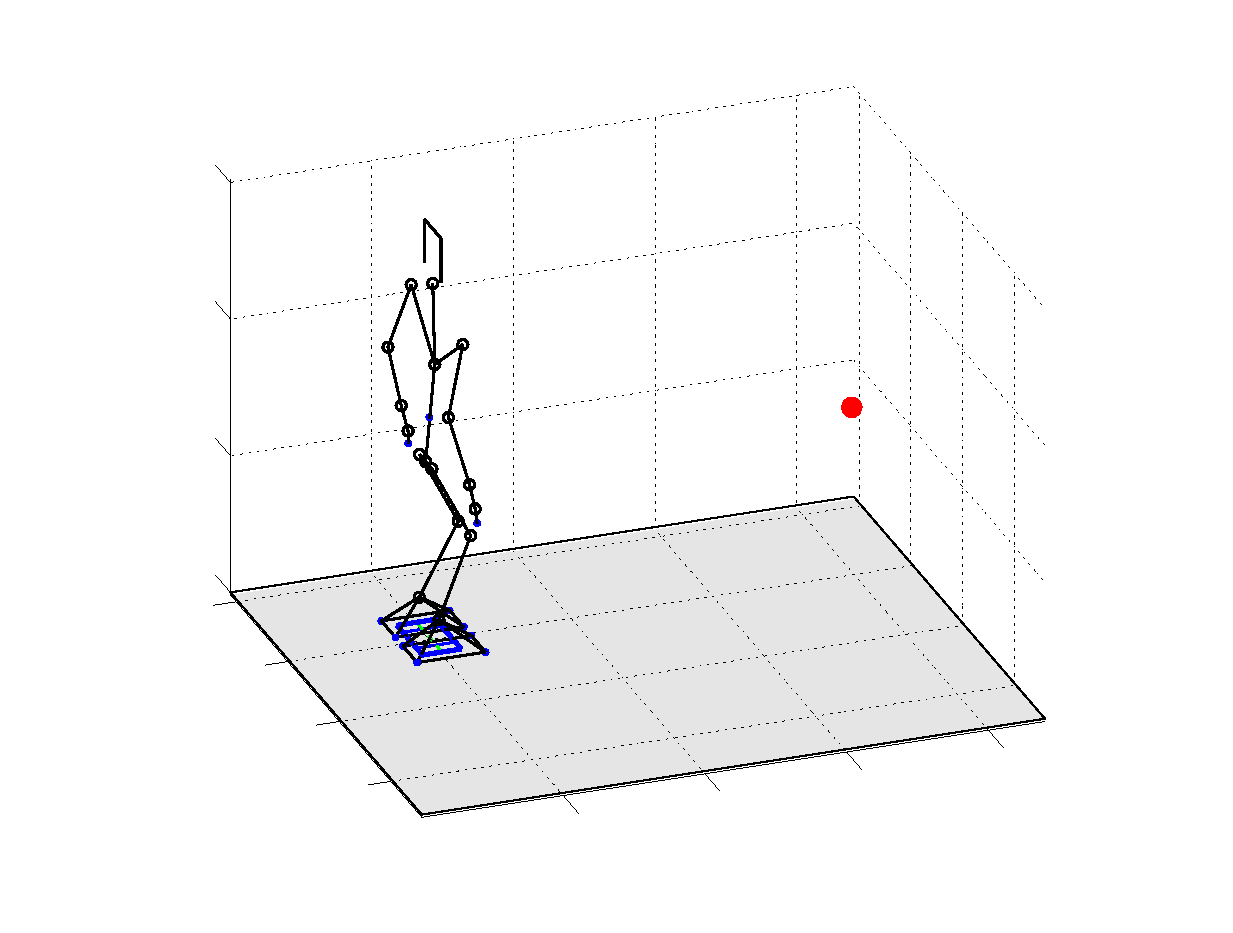
\includegraphics[trim=60  30  50   5,clip,scale=0.4]{test_16_02_robot_notermctr_1-inc}
\end{picture}%
\begin{picture}(466, 397)(60,30)
\fontsize{7}{0}
\selectfont\put(92.0583,167.716){\makebox(0,0)[br]{\textcolor[rgb]{0,0,0}{{0}}}}
\fontsize{7}{0}
\selectfont\put(92.0583,233.307){\makebox(0,0)[br]{\textcolor[rgb]{0,0,0}{{0.5}}}}
\fontsize{7}{0}
\selectfont\put(92.0583,298.899){\makebox(0,0)[br]{\textcolor[rgb]{0,0,0}{{1}}}}
\fontsize{7}{0}
\selectfont\put(92.0583,364.49){\makebox(0,0)[br]{\textcolor[rgb]{0,0,0}{{1.5}}}}
\fontsize{7}{0}
\selectfont\put(89.3552,148.531){\makebox(0,0)[tr]{\textcolor[rgb]{0,0,0}{{0.5}}}}
\fontsize{7}{0}
\selectfont\put(114.108,119.789){\makebox(0,0)[tr]{\textcolor[rgb]{0,0,0}{{0}}}}
\fontsize{7}{0}
\selectfont\put(138.861,91.048){\makebox(0,0)[tr]{\textcolor[rgb]{0,0,0}{{-0.5}}}}
\fontsize{7}{0}
\selectfont\put(163.613,62.3068){\makebox(0,0)[tr]{\textcolor[rgb]{0,0,0}{{-1}}}}
\fontsize{7}{0}
\selectfont\put(272.876,45.7507){\makebox(0,0)[tl]{\textcolor[rgb]{0,0,0}{{0}}}}
\fontsize{7}{0}
\selectfont\put(340.884,56.2116){\makebox(0,0)[tl]{\textcolor[rgb]{0,0,0}{{0.5}}}}
\fontsize{7}{0}
\selectfont\put(408.891,66.6726){\makebox(0,0)[tl]{\textcolor[rgb]{0,0,0}{{1}}}}
\fontsize{7}{0}
\selectfont\put(476.899,77.1335){\makebox(0,0)[tl]{\textcolor[rgb]{0,0,0}{{1.5}}}}
\end{picture}

            \subcaption{initial}
            \label{fig.task_walk_fall.1}
        }
    \end{minipage}
    \hfill
    \begin{minipage}[t]{0.49\textwidth}
        \centering{
            % Title: glps_renderer figure
% Creator: GL2PS 1.3.8, (C) 1999-2012 C. Geuzaine
% For: Octave
% CreationDate: Mon May  9 19:25:07 2016
\setlength{\unitlength}{0.4pt}
\begin{picture}(0,0)
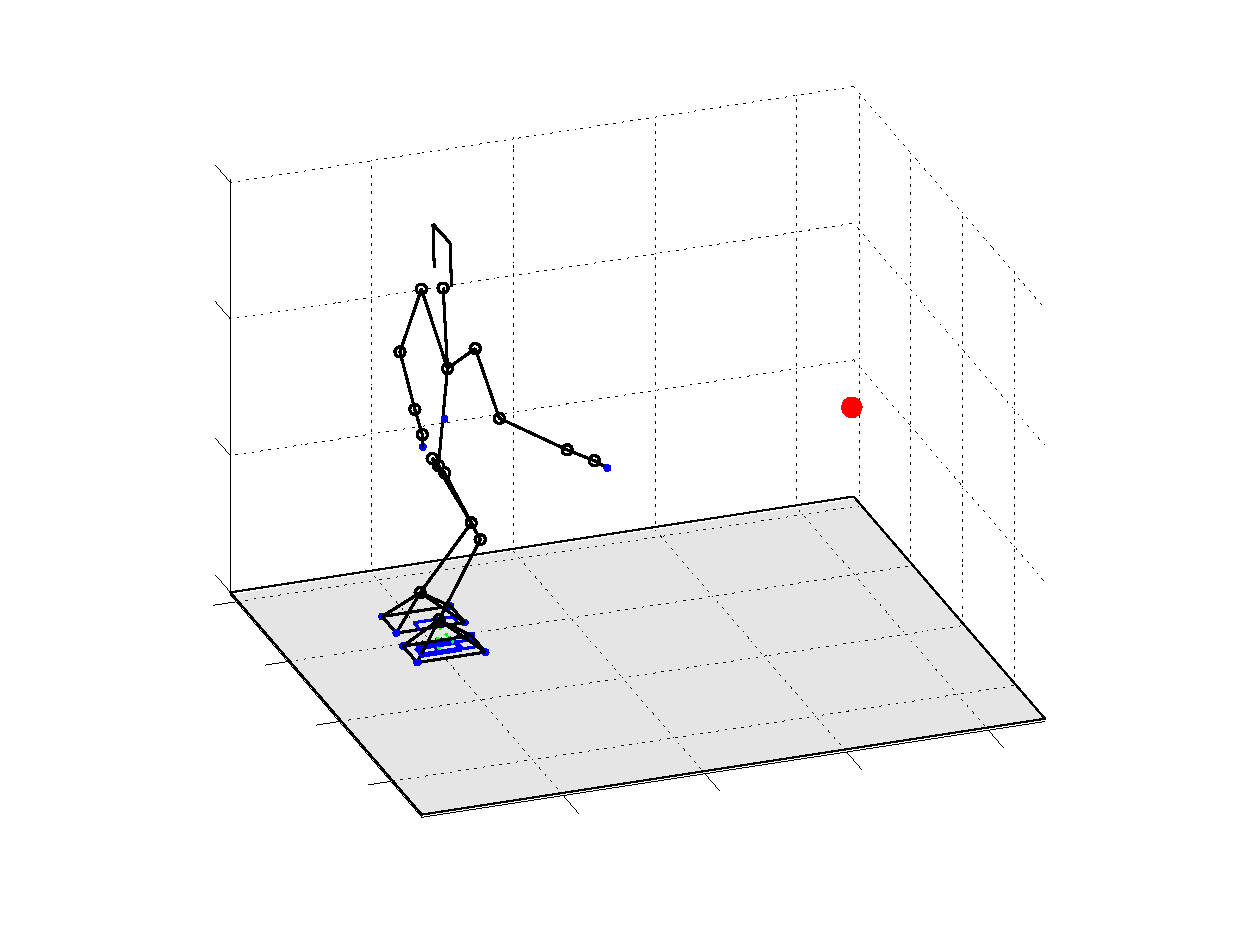
\includegraphics[trim=60  30  50   5,clip,scale=0.4]{test_16_02_robot_notermctr_101-inc}
\end{picture}%
\begin{picture}(466, 397)(60,30)
\fontsize{7}{0}
\selectfont\put(92.0583,167.716){\makebox(0,0)[br]{\textcolor[rgb]{0,0,0}{{0}}}}
\fontsize{7}{0}
\selectfont\put(92.0583,233.307){\makebox(0,0)[br]{\textcolor[rgb]{0,0,0}{{0.5}}}}
\fontsize{7}{0}
\selectfont\put(92.0583,298.899){\makebox(0,0)[br]{\textcolor[rgb]{0,0,0}{{1}}}}
\fontsize{7}{0}
\selectfont\put(92.0583,364.49){\makebox(0,0)[br]{\textcolor[rgb]{0,0,0}{{1.5}}}}
\fontsize{7}{0}
\selectfont\put(89.3552,148.531){\makebox(0,0)[tr]{\textcolor[rgb]{0,0,0}{{0.5}}}}
\fontsize{7}{0}
\selectfont\put(114.108,119.789){\makebox(0,0)[tr]{\textcolor[rgb]{0,0,0}{{0}}}}
\fontsize{7}{0}
\selectfont\put(138.861,91.048){\makebox(0,0)[tr]{\textcolor[rgb]{0,0,0}{{-0.5}}}}
\fontsize{7}{0}
\selectfont\put(163.613,62.3068){\makebox(0,0)[tr]{\textcolor[rgb]{0,0,0}{{-1}}}}
\fontsize{7}{0}
\selectfont\put(272.876,45.7507){\makebox(0,0)[tl]{\textcolor[rgb]{0,0,0}{{0}}}}
\fontsize{7}{0}
\selectfont\put(340.884,56.2116){\makebox(0,0)[tl]{\textcolor[rgb]{0,0,0}{{0.5}}}}
\fontsize{7}{0}
\selectfont\put(408.891,66.6726){\makebox(0,0)[tl]{\textcolor[rgb]{0,0,0}{{1}}}}
\fontsize{7}{0}
\selectfont\put(476.899,77.1335){\makebox(0,0)[tl]{\textcolor[rgb]{0,0,0}{{1.5}}}}
\end{picture}

            \subcaption{after $0.5$ seconds}
            \label{fig.task_walk_fall.2}
        }
    \end{minipage}
    \begin{minipage}[t]{0.49\textwidth}
        \centering{
            % Title: glps_renderer figure
% Creator: GL2PS 1.3.8, (C) 1999-2012 C. Geuzaine
% For: Octave
% CreationDate: Mon May  9 19:25:09 2016
\setlength{\unitlength}{0.4pt}
\begin{picture}(0,0)
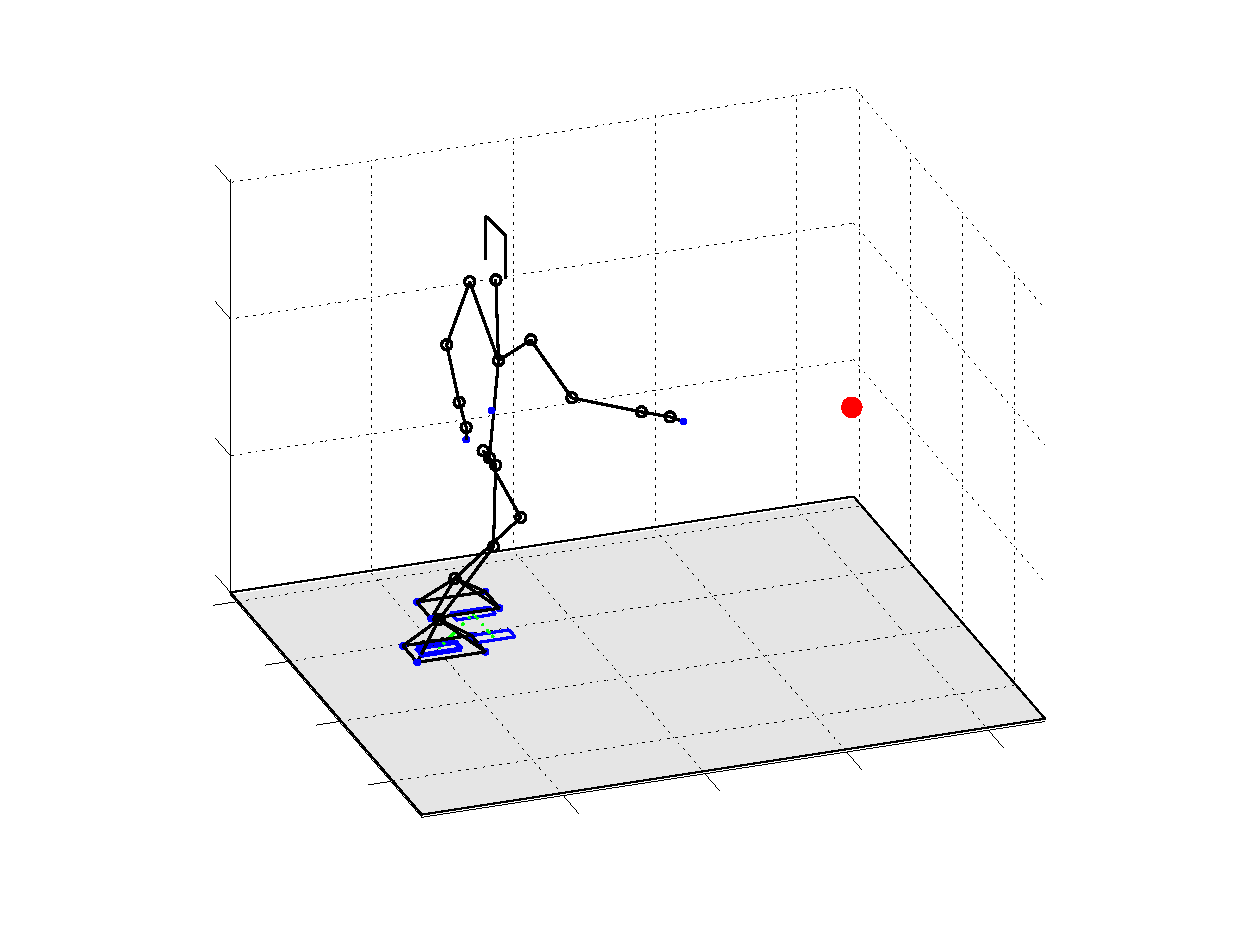
\includegraphics[trim=60  30  50   5,clip,scale=0.4]{test_16_02_robot_notermctr_176-inc}
\end{picture}%
\begin{picture}(466, 397)(60,30)
\fontsize{7}{0}
\selectfont\put(92.0583,167.716){\makebox(0,0)[br]{\textcolor[rgb]{0,0,0}{{0}}}}
\fontsize{7}{0}
\selectfont\put(92.0583,233.307){\makebox(0,0)[br]{\textcolor[rgb]{0,0,0}{{0.5}}}}
\fontsize{7}{0}
\selectfont\put(92.0583,298.899){\makebox(0,0)[br]{\textcolor[rgb]{0,0,0}{{1}}}}
\fontsize{7}{0}
\selectfont\put(92.0583,364.49){\makebox(0,0)[br]{\textcolor[rgb]{0,0,0}{{1.5}}}}
\fontsize{7}{0}
\selectfont\put(89.3552,148.531){\makebox(0,0)[tr]{\textcolor[rgb]{0,0,0}{{0.5}}}}
\fontsize{7}{0}
\selectfont\put(138.861,91.048){\makebox(0,0)[tr]{\textcolor[rgb]{0,0,0}{{-0.5}}}}
\fontsize{7}{0}
\selectfont\put(114.108,119.789){\makebox(0,0)[tr]{\textcolor[rgb]{0,0,0}{{0}}}}
\fontsize{7}{0}
\selectfont\put(476.899,77.1335){\makebox(0,0)[tl]{\textcolor[rgb]{0,0,0}{{1.5}}}}
\fontsize{7}{0}
\selectfont\put(163.613,62.3068){\makebox(0,0)[tr]{\textcolor[rgb]{0,0,0}{{-1}}}}
\fontsize{7}{0}
\selectfont\put(272.876,45.7507){\makebox(0,0)[tl]{\textcolor[rgb]{0,0,0}{{0}}}}
\fontsize{7}{0}
\selectfont\put(340.884,56.2116){\makebox(0,0)[tl]{\textcolor[rgb]{0,0,0}{{0.5}}}}
\fontsize{7}{0}
\selectfont\put(408.891,66.6726){\makebox(0,0)[tl]{\textcolor[rgb]{0,0,0}{{1}}}}
\end{picture}

            \subcaption{after $0.875$ seconds}
            \label{fig.task_walk_fall.3}
        }
    \end{minipage}
    \hfill
    \begin{minipage}[t]{0.49\textwidth}
        \centering{
            % Title: glps_renderer figure
% Creator: GL2PS 1.3.8, (C) 1999-2012 C. Geuzaine
% For: Octave
% CreationDate: Mon May  9 19:25:10 2016
\setlength{\unitlength}{0.4pt}
\begin{picture}(0,0)
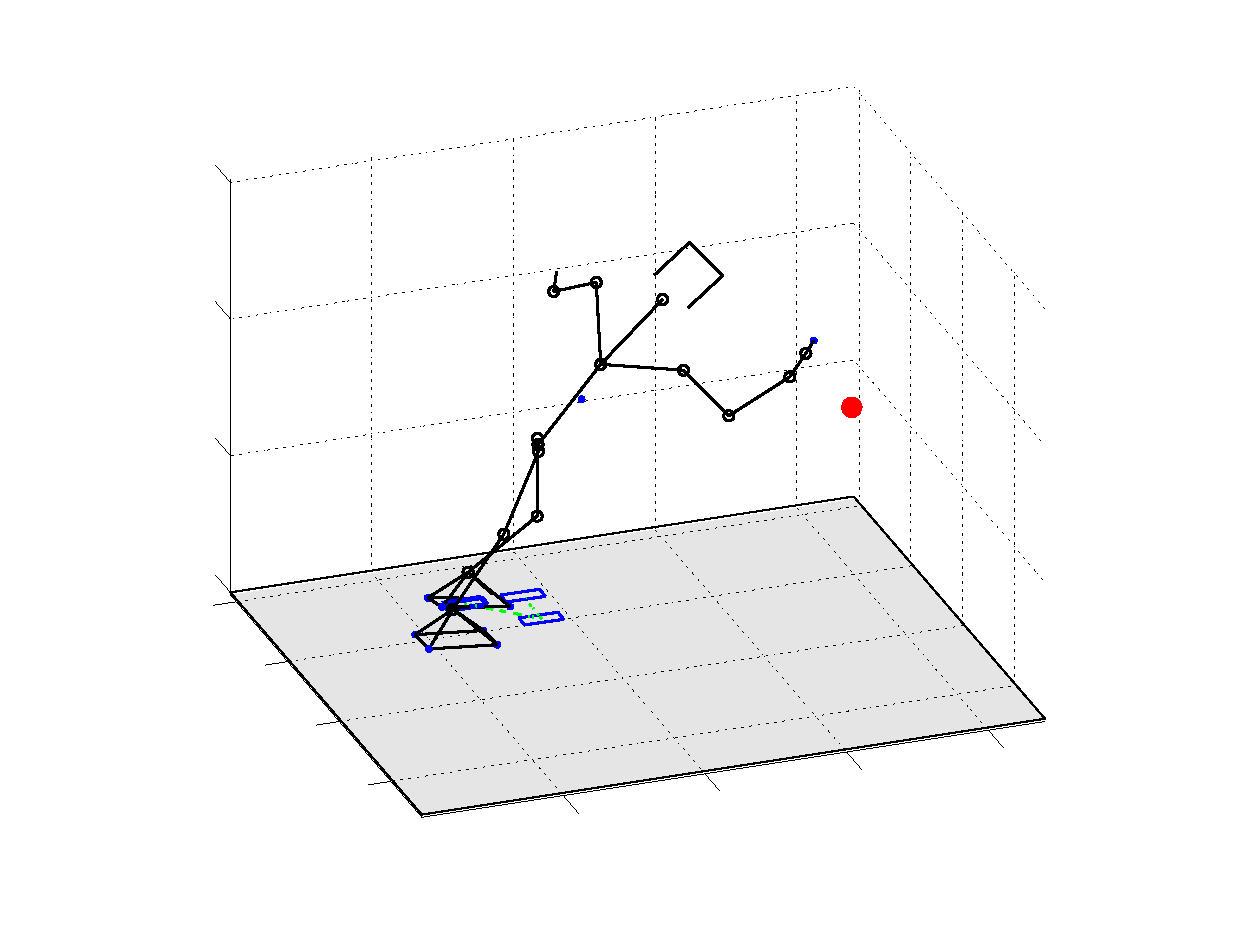
\includegraphics[trim=60  30  50   5,clip,scale=0.4]{test_16_02_robot_notermctr_250-inc}
\end{picture}%
\begin{picture}(466, 397)(60,30)
\fontsize{7}{0}
\selectfont\put(92.0583,167.716){\makebox(0,0)[br]{\textcolor[rgb]{0,0,0}{{0}}}}
\fontsize{7}{0}
\selectfont\put(92.0583,233.307){\makebox(0,0)[br]{\textcolor[rgb]{0,0,0}{{0.5}}}}
\fontsize{7}{0}
\selectfont\put(92.0583,298.899){\makebox(0,0)[br]{\textcolor[rgb]{0,0,0}{{1}}}}
\fontsize{7}{0}
\selectfont\put(92.0583,364.49){\makebox(0,0)[br]{\textcolor[rgb]{0,0,0}{{1.5}}}}
\fontsize{7}{0}
\selectfont\put(89.3552,148.531){\makebox(0,0)[tr]{\textcolor[rgb]{0,0,0}{{0.5}}}}
\fontsize{7}{0}
\selectfont\put(114.108,119.789){\makebox(0,0)[tr]{\textcolor[rgb]{0,0,0}{{0}}}}
\fontsize{7}{0}
\selectfont\put(138.861,91.048){\makebox(0,0)[tr]{\textcolor[rgb]{0,0,0}{{-0.5}}}}
\fontsize{7}{0}
\selectfont\put(163.613,62.3068){\makebox(0,0)[tr]{\textcolor[rgb]{0,0,0}{{-1}}}}
\fontsize{7}{0}
\selectfont\put(272.876,45.7507){\makebox(0,0)[tl]{\textcolor[rgb]{0,0,0}{{0}}}}
\fontsize{7}{0}
\selectfont\put(340.884,56.2116){\makebox(0,0)[tl]{\textcolor[rgb]{0,0,0}{{0.5}}}}
\fontsize{7}{0}
\selectfont\put(408.891,66.6726){\makebox(0,0)[tl]{\textcolor[rgb]{0,0,0}{{1}}}}
\fontsize{7}{0}
\selectfont\put(476.899,77.1335){\makebox(0,0)[tl]{\textcolor[rgb]{0,0,0}{{1.5}}}}
\end{picture}

            \subcaption{after $1.25$ seconds}
            \label{fig.task_walk_fall.4}
        }
    \end{minipage}
    \caption[A fall due to removal of the capturability constraint.]{
        A fall due to removal of the capturability constraint.
    }
    \label{fig.task_walk_fall}
\end{figure}


\begin{figure}[!htbp]
    \begin{minipage}[t]{\textwidth}
        \centering{
            % Title: glps_renderer figure
% Creator: GL2PS 1.3.8, (C) 1999-2012 C. Geuzaine
% For: Octave
% CreationDate: Wed Mar 30 19:27:42 2016
\setlength{\unitlength}{0.7pt}
\begin{picture}(0,0)
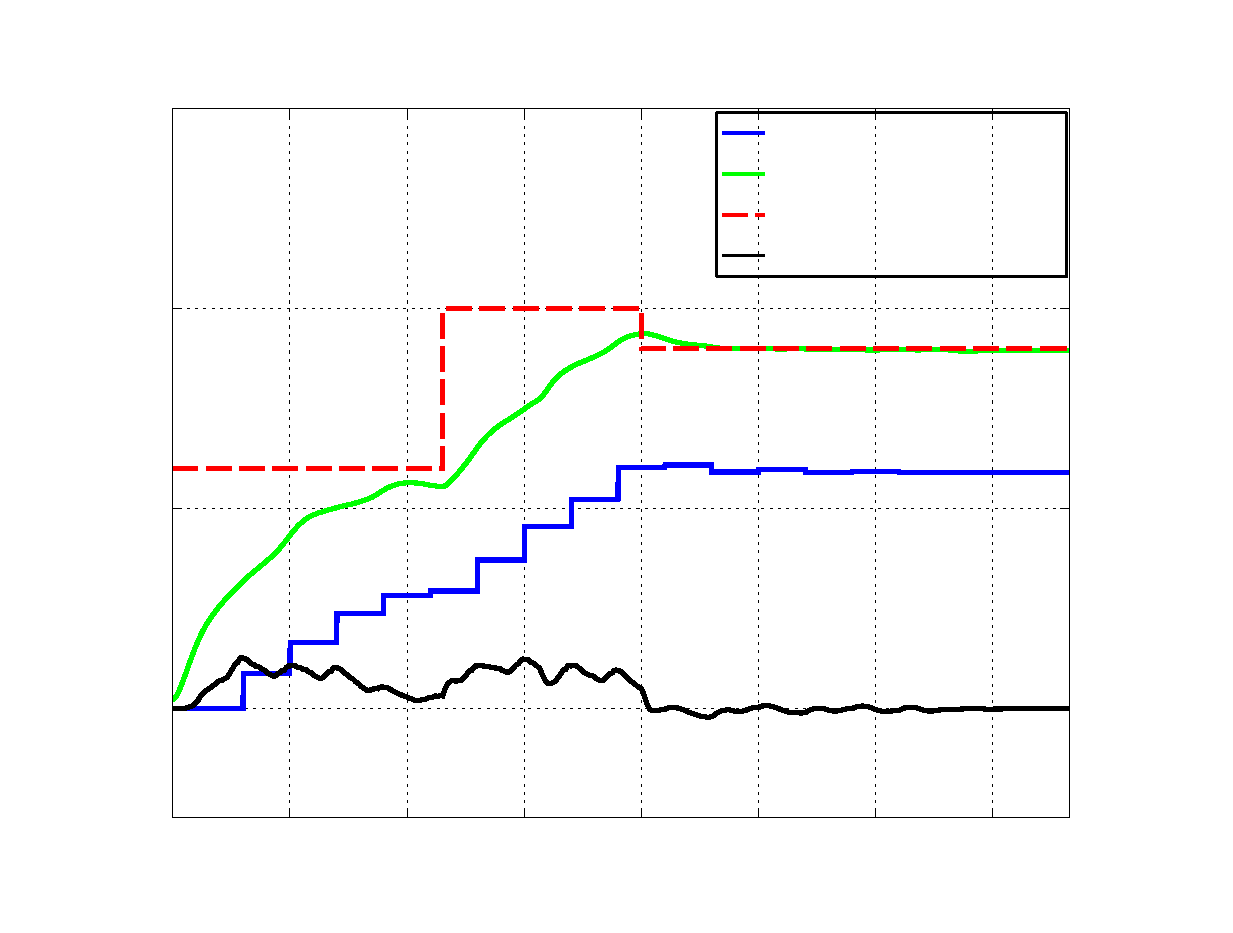
\includegraphics[trim=60   0  60  10,clip,scale=0.7]{test_16_02_XY_nodist_X_3061-inc}
\end{picture}%
\begin{picture}(456, 422)(60,0)
\fontsize{11}{0}
\selectfont\put(74.88,42.5188){\makebox(0,0)[t]{\textcolor[rgb]{0,0,0}{{0}}}}
\fontsize{11}{0}
\selectfont\put(131.123,42.5188){\makebox(0,0)[t]{\textcolor[rgb]{0,0,0}{{2}}}}
\fontsize{11}{0}
\selectfont\put(187.366,42.5188){\makebox(0,0)[t]{\textcolor[rgb]{0,0,0}{{4}}}}
\fontsize{11}{0}
\selectfont\put(243.609,42.5188){\makebox(0,0)[t]{\textcolor[rgb]{0,0,0}{{6}}}}
\fontsize{11}{0}
\selectfont\put(299.852,42.5188){\makebox(0,0)[t]{\textcolor[rgb]{0,0,0}{{8}}}}
\fontsize{11}{0}
\selectfont\put(356.095,42.5188){\makebox(0,0)[t]{\textcolor[rgb]{0,0,0}{{10}}}}
\fontsize{11}{0}
\selectfont\put(412.338,42.5188){\makebox(0,0)[t]{\textcolor[rgb]{0,0,0}{{12}}}}
\fontsize{11}{0}
\selectfont\put(468.581,42.5188){\makebox(0,0)[t]{\textcolor[rgb]{0,0,0}{{14}}}}
\fontsize{11}{0}
\selectfont\put(69.8753,99.6293){\makebox(0,0)[r]{\textcolor[rgb]{0,0,0}{{0}}}}
\fontsize{11}{0}
\selectfont\put(69.8753,195.62){\makebox(0,0)[r]{\textcolor[rgb]{0,0,0}{{1}}}}
\fontsize{11}{0}
\selectfont\put(69.8753,291.61){\makebox(0,0)[r]{\textcolor[rgb]{0,0,0}{{2}}}}
\fontsize{11}{0}
\selectfont\put(69.8753,387.6){\makebox(0,0)[r]{\textcolor[rgb]{0,0,0}{{3}}}}
\fontsize{11}{0}
\selectfont\put(290.08,31.5188){\makebox(0,0)[t]{\textcolor[rgb]{0,0,0}{{simulation time $[s]$}}}}
\fontsize{11}{0}
\selectfont\put(59.8753,217.56){\rotatebox{90}{\makebox(0,0)[b]{\textcolor[rgb]{0,0,0}{{value along the $x$ axis}}}}}
\fontsize{11}{0}
\selectfont\put(361.461,375.996){\makebox(0,0)[l]{\textcolor[rgb]{0,0,0}{{Current foot position}}}}
\fontsize{11}{0}
\selectfont\put(361.461,356.326){\makebox(0,0)[l]{\textcolor[rgb]{0,0,0}{{Right hand position}}}}
\fontsize{11}{0}
\selectfont\put(361.461,336.657){\makebox(0,0)[l]{\textcolor[rgb]{0,0,0}{{Target position}}}}
\fontsize{11}{0}
\selectfont\put(361.461,316.987){\makebox(0,0)[l]{\textcolor[rgb]{0,0,0}{{CoM velocity}}}}
\end{picture}

            \subcaption{$N = 16$, without disturbances}
            \label{fig.task_walk_x_nodist}
        }
    \end{minipage}
    \hfill
    \begin{minipage}[t]{\textwidth}
        \centering{
            % Title: glps_renderer figure
% Creator: GL2PS 1.3.8, (C) 1999-2012 C. Geuzaine
% For: Octave
% CreationDate: Wed Mar 30 19:27:39 2016
\setlength{\unitlength}{0.7pt}
\begin{picture}(0,0)
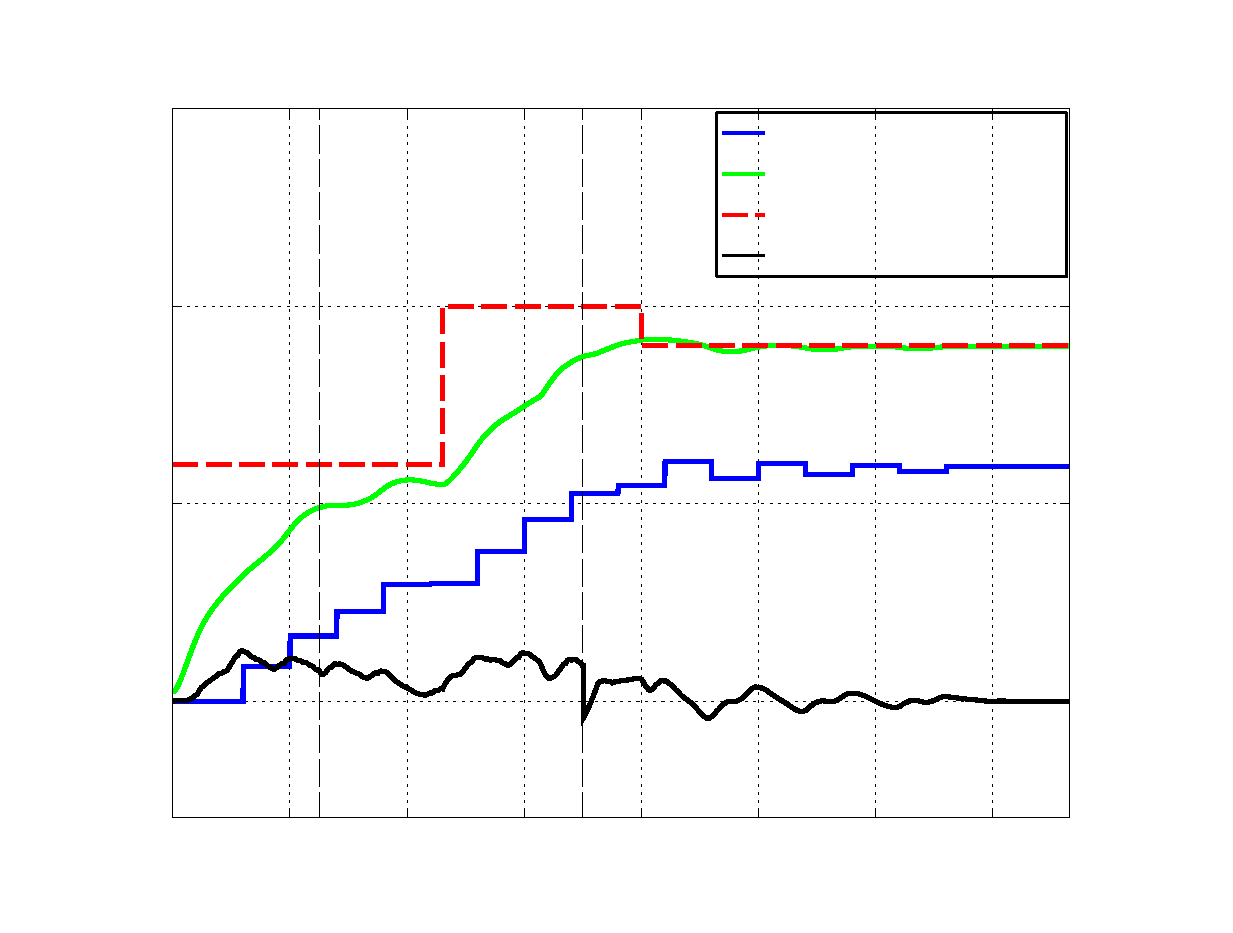
\includegraphics[trim=60   0  60  10,clip,scale=0.7]{test_16_02_XY_X_3061-inc}
\end{picture}%
\begin{picture}(456, 422)(60,0)
\fontsize{11}{0}
\selectfont\put(74.88,42.5188){\makebox(0,0)[t]{\textcolor[rgb]{0,0,0}{{0}}}}
\fontsize{11}{0}
\selectfont\put(131.123,42.5188){\makebox(0,0)[t]{\textcolor[rgb]{0,0,0}{{2}}}}
\fontsize{11}{0}
\selectfont\put(145.184,42.5188){\makebox(0,0)[t]{\textcolor[rgb]{0,0,0}{{$\impulseC_d^y$}}}}
\fontsize{11}{0}
\selectfont\put(187.366,42.5188){\makebox(0,0)[t]{\textcolor[rgb]{0,0,0}{{4}}}}
\fontsize{11}{0}
\selectfont\put(243.609,42.5188){\makebox(0,0)[t]{\textcolor[rgb]{0,0,0}{{6}}}}
\fontsize{11}{0}
\selectfont\put(271.731,42.5188){\makebox(0,0)[t]{\textcolor[rgb]{0,0,0}{{$\impulseC_d^x$}}}}
\fontsize{11}{0}
\selectfont\put(299.852,42.5188){\makebox(0,0)[t]{\textcolor[rgb]{0,0,0}{{8}}}}
\fontsize{11}{0}
\selectfont\put(356.095,42.5188){\makebox(0,0)[t]{\textcolor[rgb]{0,0,0}{{10}}}}
\fontsize{11}{0}
\selectfont\put(412.338,42.5188){\makebox(0,0)[t]{\textcolor[rgb]{0,0,0}{{12}}}}
\fontsize{11}{0}
\selectfont\put(468.581,42.5188){\makebox(0,0)[t]{\textcolor[rgb]{0,0,0}{{14}}}}
\fontsize{11}{0}
\selectfont\put(69.8753,103.277){\makebox(0,0)[r]{\textcolor[rgb]{0,0,0}{{0}}}}
\fontsize{11}{0}
\selectfont\put(69.8753,198.051){\makebox(0,0)[r]{\textcolor[rgb]{0,0,0}{{1}}}}
\fontsize{11}{0}
\selectfont\put(69.8753,292.826){\makebox(0,0)[r]{\textcolor[rgb]{0,0,0}{{2}}}}
\fontsize{11}{0}
\selectfont\put(69.8753,387.6){\makebox(0,0)[r]{\textcolor[rgb]{0,0,0}{{3}}}}
\fontsize{11}{0}
\selectfont\put(290.08,31.5188){\makebox(0,0)[t]{\textcolor[rgb]{0,0,0}{{simulation time $[s]$}}}}
\fontsize{11}{0}
\selectfont\put(59.8753,217.56){\rotatebox{90}{\makebox(0,0)[b]{\textcolor[rgb]{0,0,0}{{value along the $x$ axis}}}}}
\fontsize{11}{0}
\selectfont\put(136.747,302.303){\rotatebox{90}{\makebox(0,0)[l]{\textcolor[rgb]{0,0,0}{{disturbance}}}}}
\fontsize{11}{0}
\selectfont\put(263.294,302.303){\rotatebox{90}{\makebox(0,0)[l]{\textcolor[rgb]{0,0,0}{{disturbance}}}}}
\fontsize{11}{0}
\selectfont\put(361.461,375.996){\makebox(0,0)[l]{\textcolor[rgb]{0,0,0}{{Current foot position}}}}
\fontsize{11}{0}
\selectfont\put(361.461,356.326){\makebox(0,0)[l]{\textcolor[rgb]{0,0,0}{{Right hand position}}}}
\fontsize{11}{0}
\selectfont\put(361.461,336.657){\makebox(0,0)[l]{\textcolor[rgb]{0,0,0}{{Target position}}}}
\fontsize{11}{0}
\selectfont\put(361.461,316.987){\makebox(0,0)[l]{\textcolor[rgb]{0,0,0}{{CoM velocity}}}}
\end{picture}

            \subcaption{$N = 16$, with disturbances}
            \label{fig.task_walk_x_dist}
        }
    \end{minipage}
    \caption[Reaction to disturbances and changes of the target position ($x$ components).]{
        Evolution of the $x$ components of the target, hand, and current
        support positions and \ac{CoM} velocity with time. The time instants,
        when disturbances are applied, are indicated with vertical dashed black
        lines.
    }
    \label{fig.task_walk_x}
\end{figure}


\begin{figure}[!htbp]
    \begin{minipage}[t]{\textwidth}
        \centering{
            % Title: glps_renderer figure
% Creator: GL2PS 1.3.8, (C) 1999-2012 C. Geuzaine
% For: Octave
% CreationDate: Wed Mar 30 19:27:42 2016
\setlength{\unitlength}{0.7pt}
\begin{picture}(0,0)
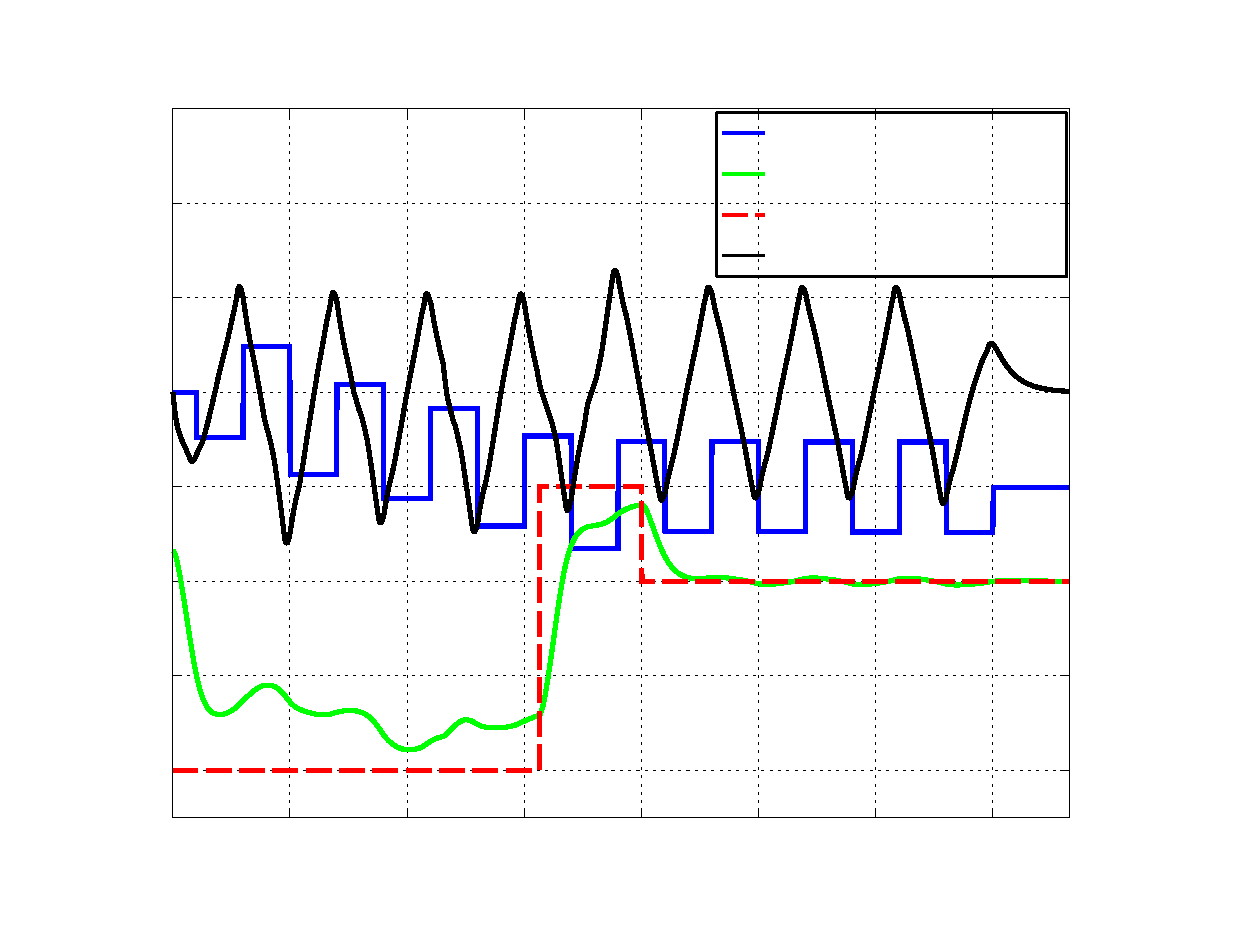
\includegraphics[trim=60   0  60  10,clip,scale=0.7]{test_16_02_XY_nodist_Y_3061-inc}
\end{picture}%
\begin{picture}(456, 422)(60,0)
\fontsize{11}{0}
\selectfont\put(74.88,42.5188){\makebox(0,0)[t]{\textcolor[rgb]{0,0,0}{{0}}}}
\fontsize{11}{0}
\selectfont\put(131.123,42.5188){\makebox(0,0)[t]{\textcolor[rgb]{0,0,0}{{2}}}}
\fontsize{11}{0}
\selectfont\put(187.366,42.5188){\makebox(0,0)[t]{\textcolor[rgb]{0,0,0}{{4}}}}
\fontsize{11}{0}
\selectfont\put(243.609,42.5188){\makebox(0,0)[t]{\textcolor[rgb]{0,0,0}{{6}}}}
\fontsize{11}{0}
\selectfont\put(299.852,42.5188){\makebox(0,0)[t]{\textcolor[rgb]{0,0,0}{{8}}}}
\fontsize{11}{0}
\selectfont\put(356.095,42.5188){\makebox(0,0)[t]{\textcolor[rgb]{0,0,0}{{10}}}}
\fontsize{11}{0}
\selectfont\put(412.338,42.5188){\makebox(0,0)[t]{\textcolor[rgb]{0,0,0}{{12}}}}
\fontsize{11}{0}
\selectfont\put(468.581,42.5188){\makebox(0,0)[t]{\textcolor[rgb]{0,0,0}{{14}}}}
\fontsize{11}{0}
\selectfont\put(69.8753,70.192){\makebox(0,0)[r]{\textcolor[rgb]{0,0,0}{{-0.8}}}}
\fontsize{11}{0}
\selectfont\put(69.8753,115.536){\makebox(0,0)[r]{\textcolor[rgb]{0,0,0}{{-0.6}}}}
\fontsize{11}{0}
\selectfont\put(69.8753,160.88){\makebox(0,0)[r]{\textcolor[rgb]{0,0,0}{{-0.4}}}}
\fontsize{11}{0}
\selectfont\put(69.8753,206.224){\makebox(0,0)[r]{\textcolor[rgb]{0,0,0}{{-0.2}}}}
\fontsize{11}{0}
\selectfont\put(69.8753,251.568){\makebox(0,0)[r]{\textcolor[rgb]{0,0,0}{{0}}}}
\fontsize{11}{0}
\selectfont\put(69.8753,296.912){\makebox(0,0)[r]{\textcolor[rgb]{0,0,0}{{0.2}}}}
\fontsize{11}{0}
\selectfont\put(69.8753,342.256){\makebox(0,0)[r]{\textcolor[rgb]{0,0,0}{{0.4}}}}
\fontsize{11}{0}
\selectfont\put(290.08,31.5188){\makebox(0,0)[t]{\textcolor[rgb]{0,0,0}{{simulation time $[s]$}}}}
\fontsize{11}{0}
\selectfont\put(47.8754,217.56){\rotatebox{90}{\makebox(0,0)[b]{\textcolor[rgb]{0,0,0}{{value along the $y$ axis}}}}}
\fontsize{11}{0}
\selectfont\put(361.461,375.996){\makebox(0,0)[l]{\textcolor[rgb]{0,0,0}{{Current foot position}}}}
\fontsize{11}{0}
\selectfont\put(361.461,356.326){\makebox(0,0)[l]{\textcolor[rgb]{0,0,0}{{Right hand position}}}}
\fontsize{11}{0}
\selectfont\put(361.461,336.657){\makebox(0,0)[l]{\textcolor[rgb]{0,0,0}{{Target position}}}}
\fontsize{11}{0}
\selectfont\put(361.461,316.987){\makebox(0,0)[l]{\textcolor[rgb]{0,0,0}{{CoM velocity}}}}
\end{picture}

            \subcaption{$N = 16$, without disturbances}
            \label{fig.task_walk_y_nodist}
        }
    \end{minipage}
    \hfill
    \begin{minipage}[t]{\textwidth}
        \centering{
            % Title: glps_renderer figure
% Creator: GL2PS 1.3.8, (C) 1999-2012 C. Geuzaine
% For: Octave
% CreationDate: Wed Mar 30 19:27:40 2016
\setlength{\unitlength}{0.7pt}
\begin{picture}(0,0)
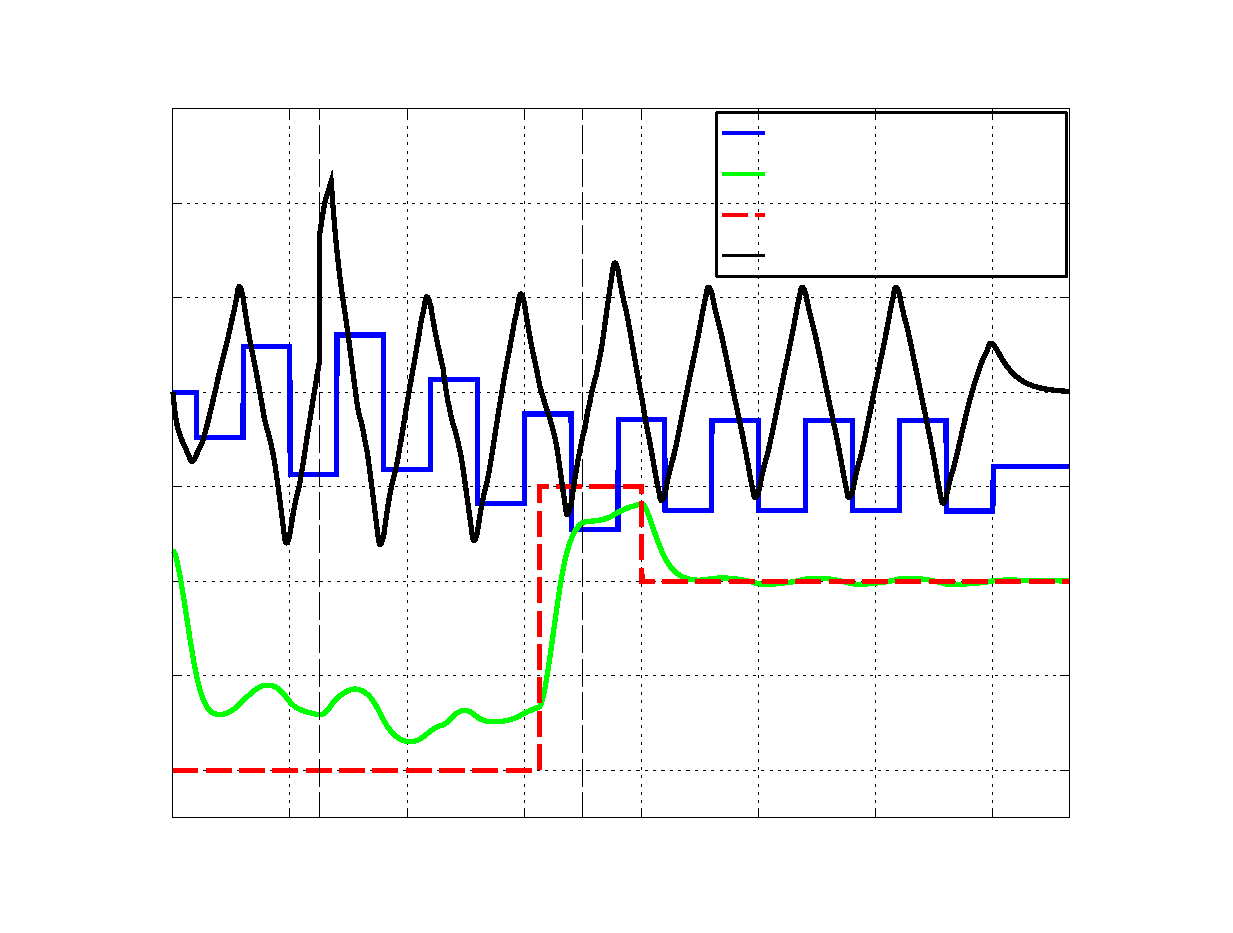
\includegraphics[trim=60   0  60  10,clip,scale=0.7]{test_16_02_XY_Y_3061-inc}
\end{picture}%
\begin{picture}(456, 422)(60,0)
\fontsize{11}{0}
\selectfont\put(74.88,42.5188){\makebox(0,0)[t]{\textcolor[rgb]{0,0,0}{{0}}}}
\fontsize{11}{0}
\selectfont\put(131.123,42.5188){\makebox(0,0)[t]{\textcolor[rgb]{0,0,0}{{2}}}}
\fontsize{11}{0}
\selectfont\put(145.184,42.5188){\makebox(0,0)[t]{\textcolor[rgb]{0,0,0}{{$\impulseC_d^y$}}}}
\fontsize{11}{0}
\selectfont\put(187.366,42.5188){\makebox(0,0)[t]{\textcolor[rgb]{0,0,0}{{4}}}}
\fontsize{11}{0}
\selectfont\put(243.609,42.5188){\makebox(0,0)[t]{\textcolor[rgb]{0,0,0}{{6}}}}
\fontsize{11}{0}
\selectfont\put(271.731,42.5188){\makebox(0,0)[t]{\textcolor[rgb]{0,0,0}{{$\impulseC_d^x$}}}}
\fontsize{11}{0}
\selectfont\put(299.852,42.5188){\makebox(0,0)[t]{\textcolor[rgb]{0,0,0}{{8}}}}
\fontsize{11}{0}
\selectfont\put(356.095,42.5188){\makebox(0,0)[t]{\textcolor[rgb]{0,0,0}{{10}}}}
\fontsize{11}{0}
\selectfont\put(412.338,42.5188){\makebox(0,0)[t]{\textcolor[rgb]{0,0,0}{{12}}}}
\fontsize{11}{0}
\selectfont\put(468.581,42.5188){\makebox(0,0)[t]{\textcolor[rgb]{0,0,0}{{14}}}}
\fontsize{11}{0}
\selectfont\put(69.8753,70.192){\makebox(0,0)[r]{\textcolor[rgb]{0,0,0}{{-0.8}}}}
\fontsize{11}{0}
\selectfont\put(69.8753,115.536){\makebox(0,0)[r]{\textcolor[rgb]{0,0,0}{{-0.6}}}}
\fontsize{11}{0}
\selectfont\put(69.8753,160.88){\makebox(0,0)[r]{\textcolor[rgb]{0,0,0}{{-0.4}}}}
\fontsize{11}{0}
\selectfont\put(69.8753,206.224){\makebox(0,0)[r]{\textcolor[rgb]{0,0,0}{{-0.2}}}}
\fontsize{11}{0}
\selectfont\put(69.8753,251.568){\makebox(0,0)[r]{\textcolor[rgb]{0,0,0}{{0}}}}
\fontsize{11}{0}
\selectfont\put(69.8753,296.912){\makebox(0,0)[r]{\textcolor[rgb]{0,0,0}{{0.2}}}}
\fontsize{11}{0}
\selectfont\put(69.8753,342.256){\makebox(0,0)[r]{\textcolor[rgb]{0,0,0}{{0.4}}}}
\fontsize{11}{0}
\selectfont\put(290.08,31.5188){\makebox(0,0)[t]{\textcolor[rgb]{0,0,0}{{simulation time $[s]$}}}}
\fontsize{11}{0}
\selectfont\put(47.8754,217.56){\rotatebox{90}{\makebox(0,0)[b]{\textcolor[rgb]{0,0,0}{{value along the $y$ axis}}}}}
\fontsize{11}{0}
\selectfont\put(136.747,310.515){\rotatebox{90}{\makebox(0,0)[l]{\textcolor[rgb]{0,0,0}{{disturbance}}}}}
\fontsize{11}{0}
\selectfont\put(263.294,310.515){\rotatebox{90}{\makebox(0,0)[l]{\textcolor[rgb]{0,0,0}{{disturbance}}}}}
\fontsize{11}{0}
\selectfont\put(361.461,375.996){\makebox(0,0)[l]{\textcolor[rgb]{0,0,0}{{Current foot position}}}}
\fontsize{11}{0}
\selectfont\put(361.461,356.326){\makebox(0,0)[l]{\textcolor[rgb]{0,0,0}{{Right hand position}}}}
\fontsize{11}{0}
\selectfont\put(361.461,336.657){\makebox(0,0)[l]{\textcolor[rgb]{0,0,0}{{Target position}}}}
\fontsize{11}{0}
\selectfont\put(361.461,316.987){\makebox(0,0)[l]{\textcolor[rgb]{0,0,0}{{CoM velocity}}}}
\end{picture}

            \subcaption{$N = 16$, with disturbances}
            \label{fig.task_walk_y_dist}
        }
    \end{minipage}
    \caption[Reaction to disturbances and changes of the target position ($y$ components).]{
        Evolution of the $y$ components of the target, hand, and current
        support positions and \ac{CoM} velocity with time. The time instants,
        when disturbances are applied, are indicated with vertical dashed black
        lines.
    }
    \label{fig.task_walk_y}
\end{figure}


\begin{figure}[!htbp]
    \begin{minipage}[t]{\textwidth}
        \centering{
            % Title: glps_renderer figure
% Creator: GL2PS 1.3.8, (C) 1999-2012 C. Geuzaine
% For: Octave
% CreationDate: Wed Mar 30 19:27:50 2016
\setlength{\unitlength}{0.7pt}
\begin{picture}(0,0)
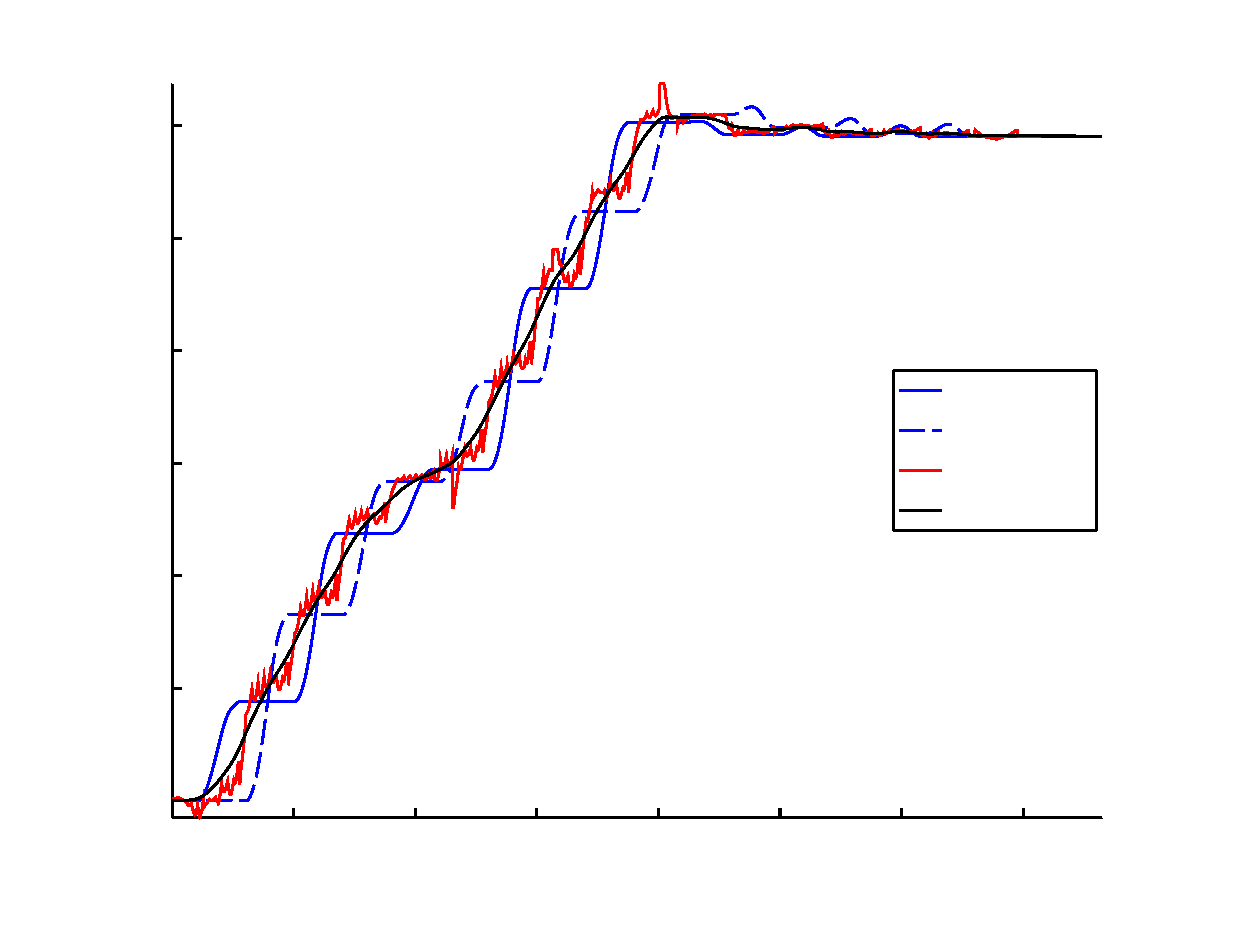
\includegraphics[trim=50   0  50  10,clip,scale=0.7]{steps_time_x_16_02_01_N16_nodist-inc}
\end{picture}%
\begin{picture}(476, 422)(50,0)
\fontsize{11}{0}
\selectfont\put(133.068,42.5189){\makebox(0,0)[t]{\textcolor[rgb]{0,0,0}{{2}}}}
\fontsize{11}{0}
\selectfont\put(191.402,42.5189){\makebox(0,0)[t]{\textcolor[rgb]{0,0,0}{{4}}}}
\fontsize{11}{0}
\selectfont\put(249.736,42.5189){\makebox(0,0)[t]{\textcolor[rgb]{0,0,0}{{6}}}}
\fontsize{11}{0}
\selectfont\put(308.07,42.5189){\makebox(0,0)[t]{\textcolor[rgb]{0,0,0}{{8}}}}
\fontsize{11}{0}
\selectfont\put(366.404,42.5189){\makebox(0,0)[t]{\textcolor[rgb]{0,0,0}{{10}}}}
\fontsize{11}{0}
\selectfont\put(424.737,42.5189){\makebox(0,0)[t]{\textcolor[rgb]{0,0,0}{{12}}}}
\fontsize{11}{0}
\selectfont\put(483.071,42.5189){\makebox(0,0)[t]{\textcolor[rgb]{0,0,0}{{14}}}}
\fontsize{11}{0}
\selectfont\put(69.8755,55.442){\makebox(0,0)[r]{\textcolor[rgb]{0,0,0}{{0}}}}
\fontsize{11}{0}
\selectfont\put(69.8755,109.463){\makebox(0,0)[r]{\textcolor[rgb]{0,0,0}{{0.2}}}}
\fontsize{11}{0}
\selectfont\put(69.8755,163.485){\makebox(0,0)[r]{\textcolor[rgb]{0,0,0}{{0.4}}}}
\fontsize{11}{0}
\selectfont\put(69.8755,217.506){\makebox(0,0)[r]{\textcolor[rgb]{0,0,0}{{0.6}}}}
\fontsize{11}{0}
\selectfont\put(69.8755,271.527){\makebox(0,0)[r]{\textcolor[rgb]{0,0,0}{{0.8}}}}
\fontsize{11}{0}
\selectfont\put(69.8755,325.549){\makebox(0,0)[r]{\textcolor[rgb]{0,0,0}{{1}}}}
\fontsize{11}{0}
\selectfont\put(69.8755,379.57){\makebox(0,0)[r]{\textcolor[rgb]{0,0,0}{{1.2}}}}
\fontsize{11}{0}
\selectfont\put(298.08,22.5189){\makebox(0,0)[t]{\textcolor[rgb]{0,0,0}{{simulation time $[s]$}}}}
\fontsize{11}{0}
\selectfont\put(40.8755,223.56){\rotatebox{90}{\makebox(0,0)[b]{\textcolor[rgb]{0,0,0}{{position along the $x$ axis $[m]$}}}}}
\fontsize{11}{0}
\selectfont\put(446.874,252.364){\makebox(0,0)[l]{\textcolor[rgb]{0,0,0}{{Left foot}}}}
\fontsize{11}{0}
\selectfont\put(446.874,233.161){\makebox(0,0)[l]{\textcolor[rgb]{0,0,0}{{Right foot}}}}
\fontsize{11}{0}
\selectfont\put(446.874,213.959){\makebox(0,0)[l]{\textcolor[rgb]{0,0,0}{{CoP}}}}
\fontsize{11}{0}
\selectfont\put(446.874,194.756){\makebox(0,0)[l]{\textcolor[rgb]{0,0,0}{{CoM}}}}
\end{picture}

            \subcaption{$N = 16$, without disturbances}
            \label{fig.task_walk_steps_time_x.nodist}
        }
    \end{minipage}
    \begin{minipage}[t]{\textwidth}
        \centering{
            % Title: glps_renderer figure
% Creator: GL2PS 1.3.8, (C) 1999-2012 C. Geuzaine
% For: Octave
% CreationDate: Wed Mar 30 19:27:48 2016
\setlength{\unitlength}{0.7pt}
\begin{picture}(0,0)
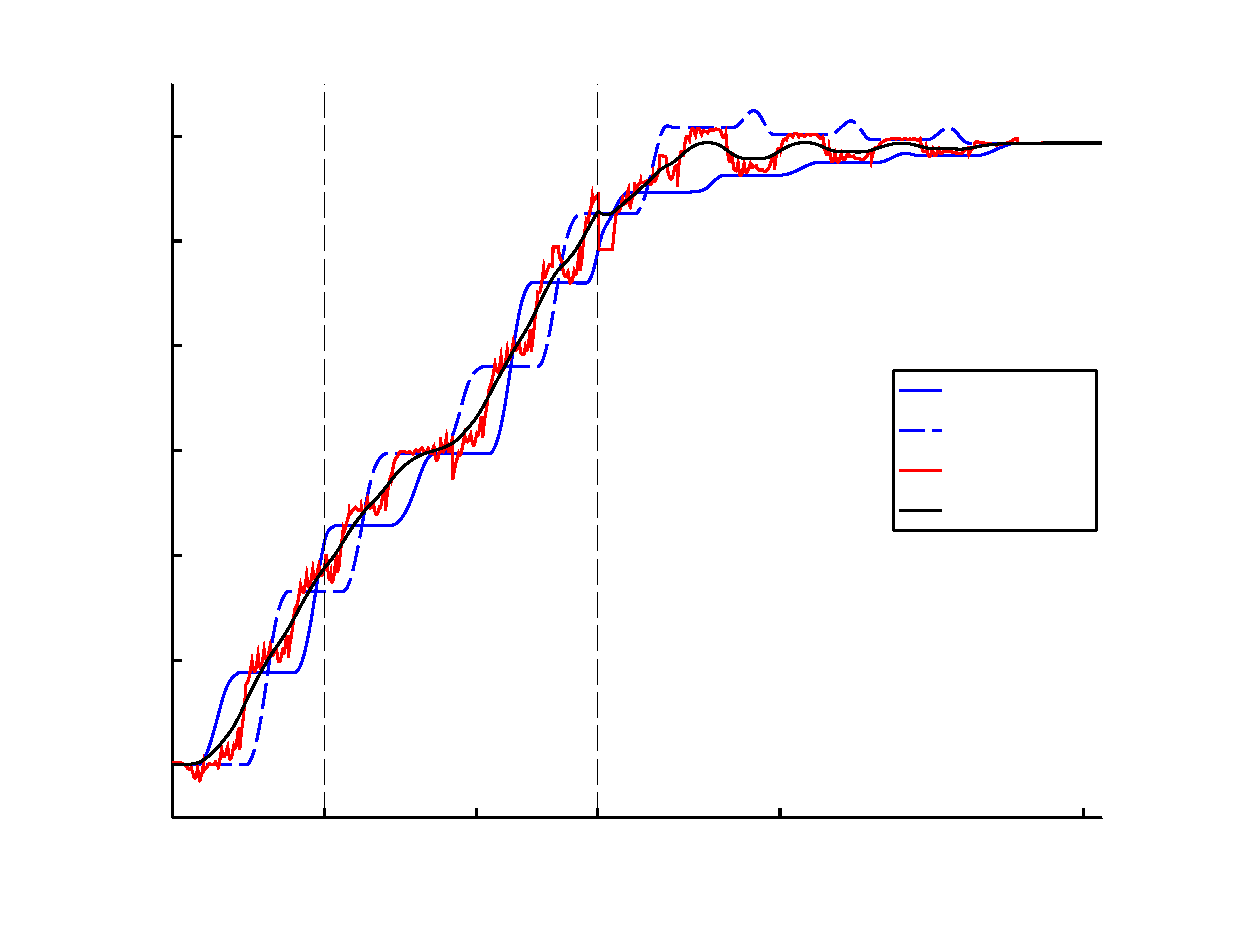
\includegraphics[trim=50   0  50  10,clip,scale=0.7]{steps_time_x_16_02_01_N16-inc}
\end{picture}%
\begin{picture}(476, 422)(50,0)
\fontsize{11}{0}
\selectfont\put(147.652,42.5189){\makebox(0,0)[t]{\textcolor[rgb]{0,0,0}{{$\impulseC_d^y$}}}}
\fontsize{11}{0}
\selectfont\put(220.569,42.5189){\makebox(0,0)[t]{\textcolor[rgb]{0,0,0}{{5}}}}
\fontsize{11}{0}
\selectfont\put(278.903,42.5189){\makebox(0,0)[t]{\textcolor[rgb]{0,0,0}{{$\impulseC_d^x$}}}}
\fontsize{11}{0}
\selectfont\put(366.404,42.5189){\makebox(0,0)[t]{\textcolor[rgb]{0,0,0}{{10}}}}
\fontsize{11}{0}
\selectfont\put(512.238,42.5189){\makebox(0,0)[t]{\textcolor[rgb]{0,0,0}{{15}}}}
\fontsize{11}{0}
\selectfont\put(69.8755,72.6686){\makebox(0,0)[r]{\textcolor[rgb]{0,0,0}{{0}}}}
\fontsize{11}{0}
\selectfont\put(69.8755,122.966){\makebox(0,0)[r]{\textcolor[rgb]{0,0,0}{{0.2}}}}
\fontsize{11}{0}
\selectfont\put(69.8755,173.263){\makebox(0,0)[r]{\textcolor[rgb]{0,0,0}{{0.4}}}}
\fontsize{11}{0}
\selectfont\put(69.8755,223.56){\makebox(0,0)[r]{\textcolor[rgb]{0,0,0}{{0.6}}}}
\fontsize{11}{0}
\selectfont\put(69.8755,273.857){\makebox(0,0)[r]{\textcolor[rgb]{0,0,0}{{0.8}}}}
\fontsize{11}{0}
\selectfont\put(69.8755,324.154){\makebox(0,0)[r]{\textcolor[rgb]{0,0,0}{{1}}}}
\fontsize{11}{0}
\selectfont\put(69.8755,374.451){\makebox(0,0)[r]{\textcolor[rgb]{0,0,0}{{1.2}}}}
\fontsize{11}{0}
\selectfont\put(298.08,22.5189){\makebox(0,0)[t]{\textcolor[rgb]{0,0,0}{{simulation time $[s]$}}}}
\fontsize{11}{0}
\selectfont\put(40.8755,223.56){\rotatebox{90}{\makebox(0,0)[b]{\textcolor[rgb]{0,0,0}{{position along the $x$ axis $[m]$}}}}}
\fontsize{11}{0}
\selectfont\put(446.874,252.364){\makebox(0,0)[l]{\textcolor[rgb]{0,0,0}{{Left foot}}}}
\fontsize{11}{0}
\selectfont\put(446.874,233.161){\makebox(0,0)[l]{\textcolor[rgb]{0,0,0}{{Right foot}}}}
\fontsize{11}{0}
\selectfont\put(446.874,213.959){\makebox(0,0)[l]{\textcolor[rgb]{0,0,0}{{CoP}}}}
\fontsize{11}{0}
\selectfont\put(446.874,194.756){\makebox(0,0)[l]{\textcolor[rgb]{0,0,0}{{CoM}}}}
\end{picture}

            \subcaption{$N = 16$, with disturbances}
            \label{fig.task_walk_steps_time_x.dist}
        }
    \end{minipage}
    \caption[Evolution of the feet, CoM, and CoP positions with time along the $x$ axis.]{
        Evolution of the positions of feet, \ac{CoM}, and \ac{CoP} with time
        along the $x$ axis. The time instants, when disturbances are applied,
        are indicated with vertical dashed black lines.
    }
    \label{fig.task_walk_steps_time_x}
\end{figure}


\begin{figure}[!htbp]
    \begin{minipage}[t]{\textwidth}
        \centering{
            % Title: glps_renderer figure
% Creator: GL2PS 1.3.8, (C) 1999-2012 C. Geuzaine
% For: Octave
% CreationDate: Wed Mar 30 19:27:51 2016
\setlength{\unitlength}{0.7pt}
\begin{picture}(0,0)
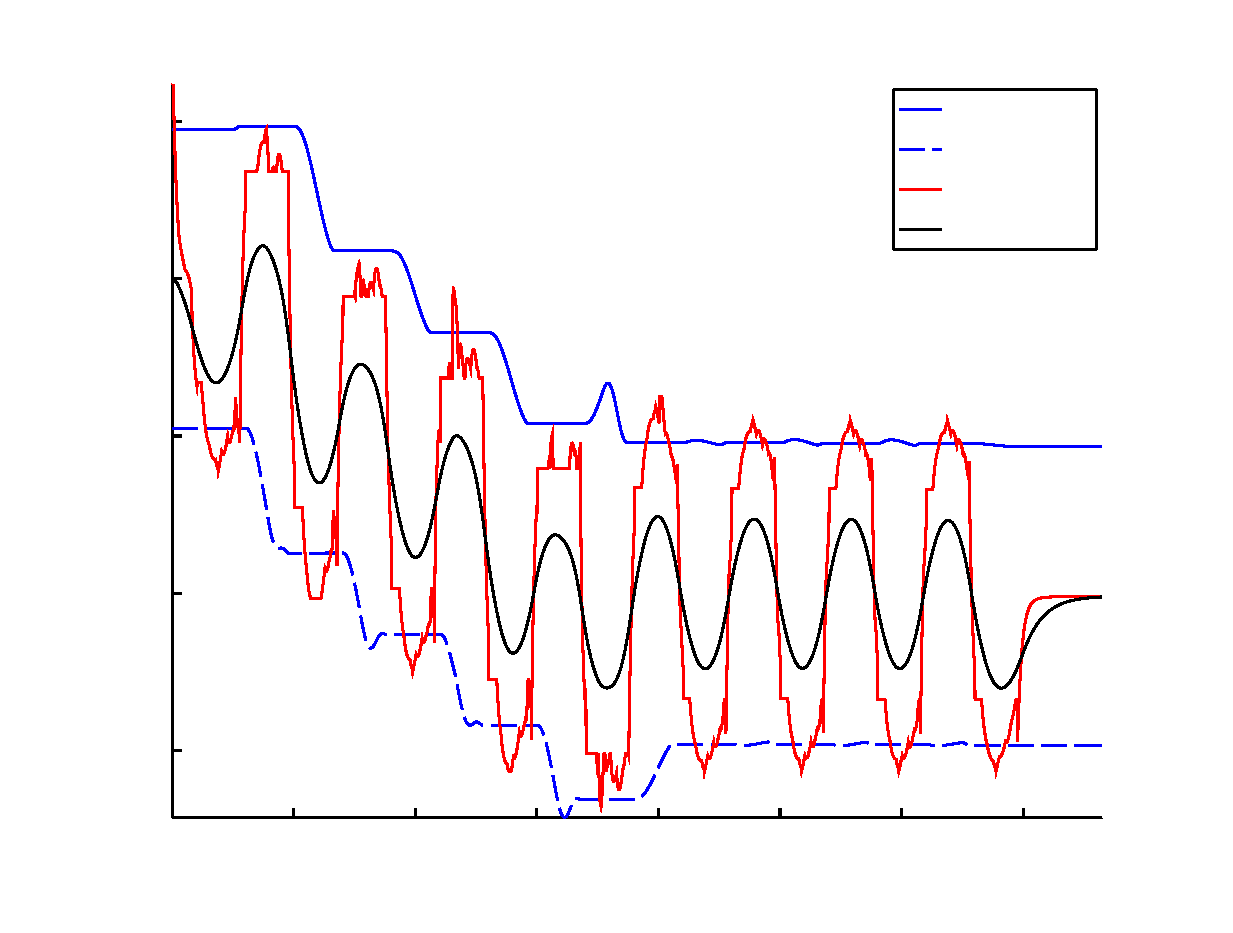
\includegraphics[trim=50   0  50  10,clip,scale=0.7]{steps_time_y_16_02_01_N16_nodist-inc}
\end{picture}%
\begin{picture}(476, 422)(50,0)
\fontsize{11}{0}
\selectfont\put(133.068,42.5189){\makebox(0,0)[t]{\textcolor[rgb]{0,0,0}{{2}}}}
\fontsize{11}{0}
\selectfont\put(191.402,42.5189){\makebox(0,0)[t]{\textcolor[rgb]{0,0,0}{{4}}}}
\fontsize{11}{0}
\selectfont\put(249.736,42.5189){\makebox(0,0)[t]{\textcolor[rgb]{0,0,0}{{6}}}}
\fontsize{11}{0}
\selectfont\put(308.07,42.5189){\makebox(0,0)[t]{\textcolor[rgb]{0,0,0}{{8}}}}
\fontsize{11}{0}
\selectfont\put(366.404,42.5189){\makebox(0,0)[t]{\textcolor[rgb]{0,0,0}{{10}}}}
\fontsize{11}{0}
\selectfont\put(424.737,42.5189){\makebox(0,0)[t]{\textcolor[rgb]{0,0,0}{{12}}}}
\fontsize{11}{0}
\selectfont\put(483.071,42.5189){\makebox(0,0)[t]{\textcolor[rgb]{0,0,0}{{14}}}}
\fontsize{11}{0}
\selectfont\put(69.8755,79.6517){\makebox(0,0)[r]{\textcolor[rgb]{0,0,0}{{-0.3}}}}
\fontsize{11}{0}
\selectfont\put(69.8755,155.111){\makebox(0,0)[r]{\textcolor[rgb]{0,0,0}{{-0.2}}}}
\fontsize{11}{0}
\selectfont\put(69.8755,230.571){\makebox(0,0)[r]{\textcolor[rgb]{0,0,0}{{-0.1}}}}
\fontsize{11}{0}
\selectfont\put(69.8755,306.03){\makebox(0,0)[r]{\textcolor[rgb]{0,0,0}{{0}}}}
\fontsize{11}{0}
\selectfont\put(69.8755,381.489){\makebox(0,0)[r]{\textcolor[rgb]{0,0,0}{{0.1}}}}
\fontsize{11}{0}
\selectfont\put(298.08,22.5189){\makebox(0,0)[t]{\textcolor[rgb]{0,0,0}{{simulation time $[s]$}}}}
\fontsize{11}{0}
\selectfont\put(34.8755,223.56){\rotatebox{90}{\makebox(0,0)[b]{\textcolor[rgb]{0,0,0}{{position along the $y$ axis $[m]$}}}}}
\fontsize{11}{0}
\selectfont\put(446.874,387.253){\makebox(0,0)[l]{\textcolor[rgb]{0,0,0}{{Left foot}}}}
\fontsize{11}{0}
\selectfont\put(446.874,368.05){\makebox(0,0)[l]{\textcolor[rgb]{0,0,0}{{Right foot}}}}
\fontsize{11}{0}
\selectfont\put(446.874,348.847){\makebox(0,0)[l]{\textcolor[rgb]{0,0,0}{{CoP}}}}
\fontsize{11}{0}
\selectfont\put(446.874,329.644){\makebox(0,0)[l]{\textcolor[rgb]{0,0,0}{{CoM}}}}
\end{picture}

            \subcaption{$N = 16$, without disturbances}
            \label{fig.task_walk_steps_time_y.nodist}
        }
    \end{minipage}
    \begin{minipage}[t]{\textwidth}
        \centering{
            % Title: glps_renderer figure
% Creator: GL2PS 1.3.8, (C) 1999-2012 C. Geuzaine
% For: Octave
% CreationDate: Wed Mar 30 19:27:48 2016
\setlength{\unitlength}{0.7pt}
\begin{picture}(0,0)
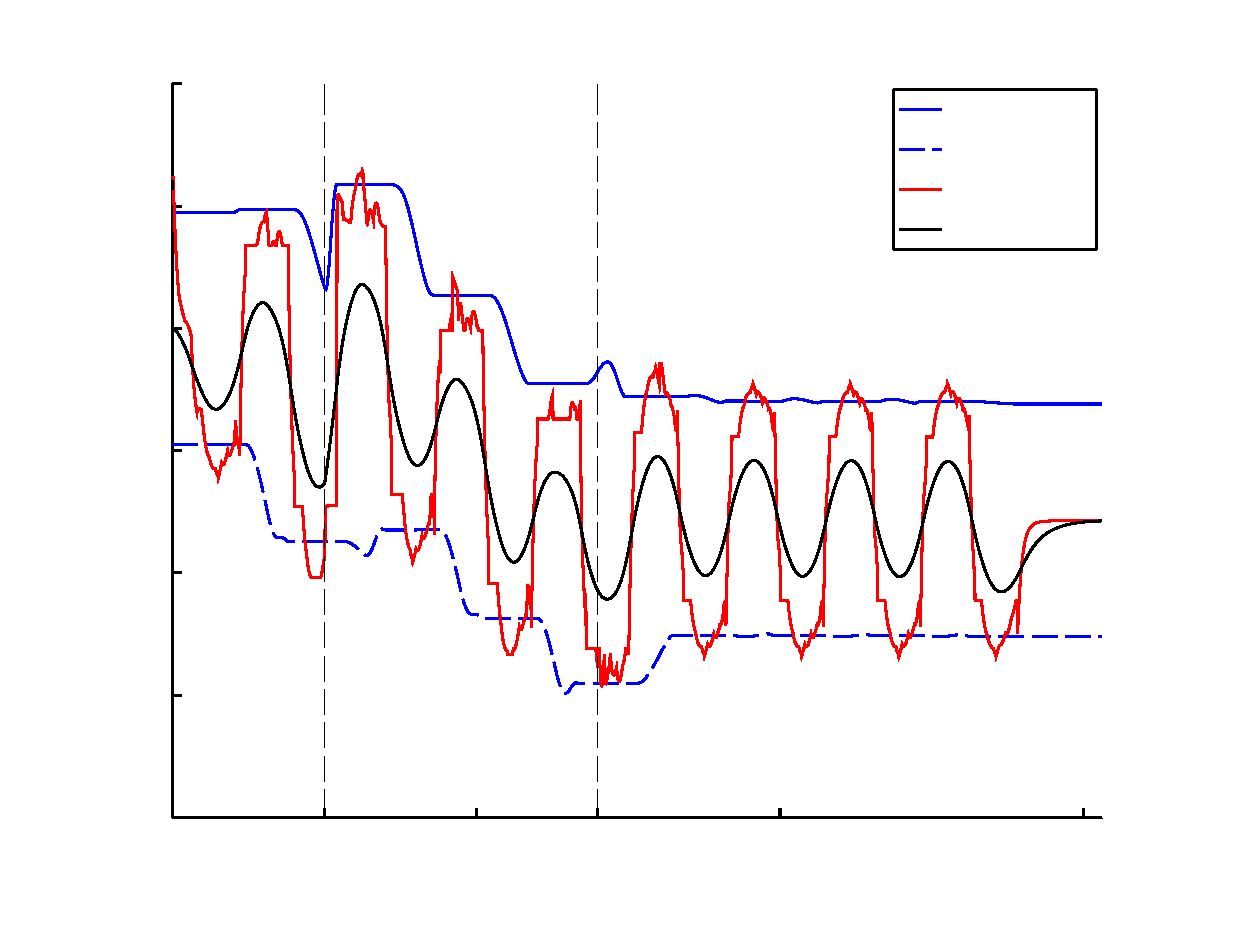
\includegraphics[trim=50   0  50  10,clip,scale=0.7]{steps_time_y_16_02_01_N16-inc}
\end{picture}%
\begin{picture}(476, 422)(50,0)
\fontsize{11}{0}
\selectfont\put(147.652,42.5189){\makebox(0,0)[t]{\textcolor[rgb]{0,0,0}{{$\impulseC_d^y$}}}}
\fontsize{11}{0}
\selectfont\put(220.569,42.5189){\makebox(0,0)[t]{\textcolor[rgb]{0,0,0}{{5}}}}
\fontsize{11}{0}
\selectfont\put(278.903,42.5189){\makebox(0,0)[t]{\textcolor[rgb]{0,0,0}{{$\impulseC_d^x$}}}}
\fontsize{11}{0}
\selectfont\put(366.404,42.5189){\makebox(0,0)[t]{\textcolor[rgb]{0,0,0}{{10}}}}
\fontsize{11}{0}
\selectfont\put(512.238,42.5189){\makebox(0,0)[t]{\textcolor[rgb]{0,0,0}{{15}}}}
\fontsize{11}{0}
\selectfont\put(69.8755,47.52){\makebox(0,0)[r]{\textcolor[rgb]{0,0,0}{{-0.4}}}}
\fontsize{11}{0}
\selectfont\put(69.8755,106.2){\makebox(0,0)[r]{\textcolor[rgb]{0,0,0}{{-0.3}}}}
\fontsize{11}{0}
\selectfont\put(69.8755,164.88){\makebox(0,0)[r]{\textcolor[rgb]{0,0,0}{{-0.2}}}}
\fontsize{11}{0}
\selectfont\put(69.8755,223.56){\makebox(0,0)[r]{\textcolor[rgb]{0,0,0}{{-0.1}}}}
\fontsize{11}{0}
\selectfont\put(69.8755,282.24){\makebox(0,0)[r]{\textcolor[rgb]{0,0,0}{{0}}}}
\fontsize{11}{0}
\selectfont\put(69.8755,340.92){\makebox(0,0)[r]{\textcolor[rgb]{0,0,0}{{0.1}}}}
\fontsize{11}{0}
\selectfont\put(69.8755,399.6){\makebox(0,0)[r]{\textcolor[rgb]{0,0,0}{{0.2}}}}
\fontsize{11}{0}
\selectfont\put(298.08,22.5189){\makebox(0,0)[t]{\textcolor[rgb]{0,0,0}{{simulation time $[s]$}}}}
\fontsize{11}{0}
\selectfont\put(34.8755,223.56){\rotatebox{90}{\makebox(0,0)[b]{\textcolor[rgb]{0,0,0}{{position along the $y$ axis $[m]$}}}}}
\fontsize{11}{0}
\selectfont\put(446.874,387.253){\makebox(0,0)[l]{\textcolor[rgb]{0,0,0}{{Left foot}}}}
\fontsize{11}{0}
\selectfont\put(446.874,368.05){\makebox(0,0)[l]{\textcolor[rgb]{0,0,0}{{Right foot}}}}
\fontsize{11}{0}
\selectfont\put(446.874,348.847){\makebox(0,0)[l]{\textcolor[rgb]{0,0,0}{{CoP}}}}
\fontsize{11}{0}
\selectfont\put(446.874,329.644){\makebox(0,0)[l]{\textcolor[rgb]{0,0,0}{{CoM}}}}
\end{picture}

            \subcaption{$N = 16$, with disturbances}
            \label{fig.task_walk_steps_time_y.dist}
        }
    \end{minipage}
    \caption[Evolution of the feet, CoM, and CoP positions with time along the $y$ axis.]{
        Evolution of the positions of feet, \ac{CoM}, and \ac{CoP} with time
        along the $y$ axis. The time instants, when disturbances are applied,
        are indicated with vertical dashed black lines.
    }
    \label{fig.task_walk_steps_time_y}
\end{figure}


Balanced walking motions can be obtained without a capturability constraint
provided that the weights of the objectives are properly tuned
\cite{Wieber2008iros,Herdt2010auro}. However, addition of such constraint makes
controller less sensitive to the weights. For example, the considered \ac{MMPC}
controller makes the robot fall in the very beginning of the simulation, when
the capturability constraint is omitted (see \cref{fig.task_walk_fall}).
Though, it is possible to adjust objectives on the last level of the hierarchy
and their weights to avoid this, it is unnecessary due to the capturability
constraint.


Satisfaction of the capturability constraint, however, does not guarantee that
the balance is always preserved. We observed that introduction of an additional
level in the hierarchy in order to prioritize the hand task over other tasks of
the last level leads to violent motions of the upper body and, eventually, to a
fall. We believe that the reason for this is that the point-mass approximation
does not reflect the complex dynamics of the robot to a necessary extent.
Hence, approximate models including angular momentum may be more appropriate
for the considered setting.




%%%%%%%%%%%%%%%%%%%%%%%%%%%%%%%%%%%%%%%%%%%%%%%%%%%%%%%%%%%%%%%%%%%%%%%%%%%%%%%%
\subsubsection{Computational performance of \sn{LexLS}}\label{sec.walk_performance}

\vspace{-0.5cm}
\begin{figure*}[!htb]
    \begin{minipage}[t]{0.49\textwidth}
        \centering{
            % Title: glps_renderer figure
% Creator: GL2PS 1.3.8, (C) 1999-2012 C. Geuzaine
% For: Octave
% CreationDate: Wed Mar 23 19:36:50 2016
\setlength{\unitlength}{0.42pt}
\begin{picture}(0,0)
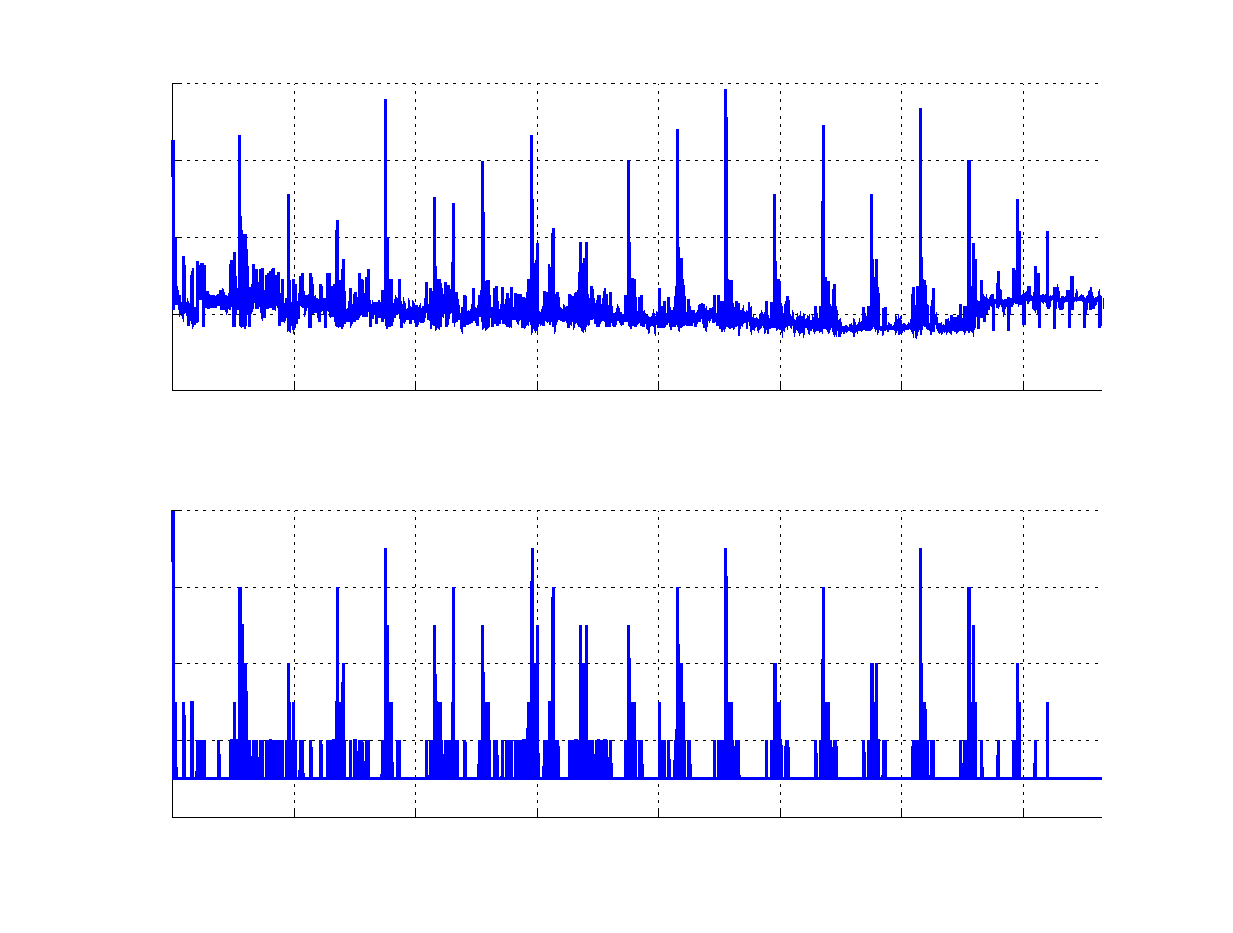
\includegraphics[trim=30  20   0   0,clip,scale=0.42]{time_16_02_03_N16_nodist-inc}
\end{picture}%
\begin{picture}(546, 412)(30,20)
\fontsize{8}{0}
\selectfont\put(74.88,247.205){\makebox(0,0)[t]{\textcolor[rgb]{0,0,0}{{0}}}}
\fontsize{8}{0}
\selectfont\put(133.214,247.205){\makebox(0,0)[t]{\textcolor[rgb]{0,0,0}{{2}}}}
\fontsize{8}{0}
\selectfont\put(191.548,247.205){\makebox(0,0)[t]{\textcolor[rgb]{0,0,0}{{4}}}}
\fontsize{8}{0}
\selectfont\put(249.882,247.205){\makebox(0,0)[t]{\textcolor[rgb]{0,0,0}{{6}}}}
\fontsize{8}{0}
\selectfont\put(308.216,247.205){\makebox(0,0)[t]{\textcolor[rgb]{0,0,0}{{8}}}}
\fontsize{8}{0}
\selectfont\put(366.549,247.205){\makebox(0,0)[t]{\textcolor[rgb]{0,0,0}{{10}}}}
\fontsize{8}{0}
\selectfont\put(424.883,247.205){\makebox(0,0)[t]{\textcolor[rgb]{0,0,0}{{12}}}}
\fontsize{8}{0}
\selectfont\put(483.217,247.205){\makebox(0,0)[t]{\textcolor[rgb]{0,0,0}{{14}}}}
\fontsize{8}{0}
\selectfont\put(69.8755,252.218){\makebox(0,0)[r]{\textcolor[rgb]{0,0,0}{{0}}}}
\fontsize{8}{0}
\selectfont\put(69.8755,289.063){\makebox(0,0)[r]{\textcolor[rgb]{0,0,0}{{1}}}}
\fontsize{8}{0}
\selectfont\put(69.8755,325.909){\makebox(0,0)[r]{\textcolor[rgb]{0,0,0}{{2}}}}
\fontsize{8}{0}
\selectfont\put(69.8755,362.754){\makebox(0,0)[r]{\textcolor[rgb]{0,0,0}{{3}}}}
\fontsize{8}{0}
\selectfont\put(69.8755,399.6){\makebox(0,0)[r]{\textcolor[rgb]{0,0,0}{{4}}}}
\fontsize{8}{0}
\selectfont\put(48.8755,325.909){\rotatebox{90}{\makebox(0,0)[b]{\textcolor[rgb]{0,0,0}{{comp. time $[ms]$}}}}}
\fontsize{8}{0}
\selectfont\put(74.88,42.507){\makebox(0,0)[t]{\textcolor[rgb]{0,0,0}{{0}}}}
\fontsize{8}{0}
\selectfont\put(133.214,42.507){\makebox(0,0)[t]{\textcolor[rgb]{0,0,0}{{2}}}}
\fontsize{8}{0}
\selectfont\put(191.548,42.507){\makebox(0,0)[t]{\textcolor[rgb]{0,0,0}{{4}}}}
\fontsize{8}{0}
\selectfont\put(249.882,42.507){\makebox(0,0)[t]{\textcolor[rgb]{0,0,0}{{6}}}}
\fontsize{8}{0}
\selectfont\put(308.216,42.507){\makebox(0,0)[t]{\textcolor[rgb]{0,0,0}{{8}}}}
\fontsize{8}{0}
\selectfont\put(366.549,42.507){\makebox(0,0)[t]{\textcolor[rgb]{0,0,0}{{10}}}}
\fontsize{8}{0}
\selectfont\put(424.883,42.507){\makebox(0,0)[t]{\textcolor[rgb]{0,0,0}{{12}}}}
\fontsize{8}{0}
\selectfont\put(483.217,42.507){\makebox(0,0)[t]{\textcolor[rgb]{0,0,0}{{14}}}}
\fontsize{8}{0}
\selectfont\put(69.8755,47.52){\makebox(0,0)[r]{\textcolor[rgb]{0,0,0}{{0}}}}
\fontsize{8}{0}
\selectfont\put(69.8755,84.3656){\makebox(0,0)[r]{\textcolor[rgb]{0,0,0}{{2}}}}
\fontsize{8}{0}
\selectfont\put(69.8755,121.211){\makebox(0,0)[r]{\textcolor[rgb]{0,0,0}{{4}}}}
\fontsize{8}{0}
\selectfont\put(69.8755,158.057){\makebox(0,0)[r]{\textcolor[rgb]{0,0,0}{{6}}}}
\fontsize{8}{0}
\selectfont\put(69.8755,194.902){\makebox(0,0)[r]{\textcolor[rgb]{0,0,0}{{8}}}}
\fontsize{8}{0}
\selectfont\put(298.08,9.50697){\makebox(0,0)[t]{\textcolor[rgb]{0,0,0}{{simulation time $[s]$}}}}
\fontsize{8}{0}
\selectfont\put(48.8755,121.211){\rotatebox{90}{\makebox(0,0)[b]{\textcolor[rgb]{0,0,0}{{num. of iterations}}}}}
\end{picture}

            \subcaption{
                $N = 16$, without disturbances.\\
                Mean computational time: $1.04~[\MT{ms}]$.\\
                Time measurements $> 1~[\MT{ms}]$: 49\%
            }
            \label{fig.task_walk_time.1}
        }
    \end{minipage}
    \hfill
    \begin{minipage}[t]{0.49\textwidth}
        \centering{
            % Title: glps_renderer figure
% Creator: GL2PS 1.3.8, (C) 1999-2012 C. Geuzaine
% For: Octave
% CreationDate: Wed Mar 23 19:36:49 2016
\setlength{\unitlength}{0.42pt}
\begin{picture}(0,0)
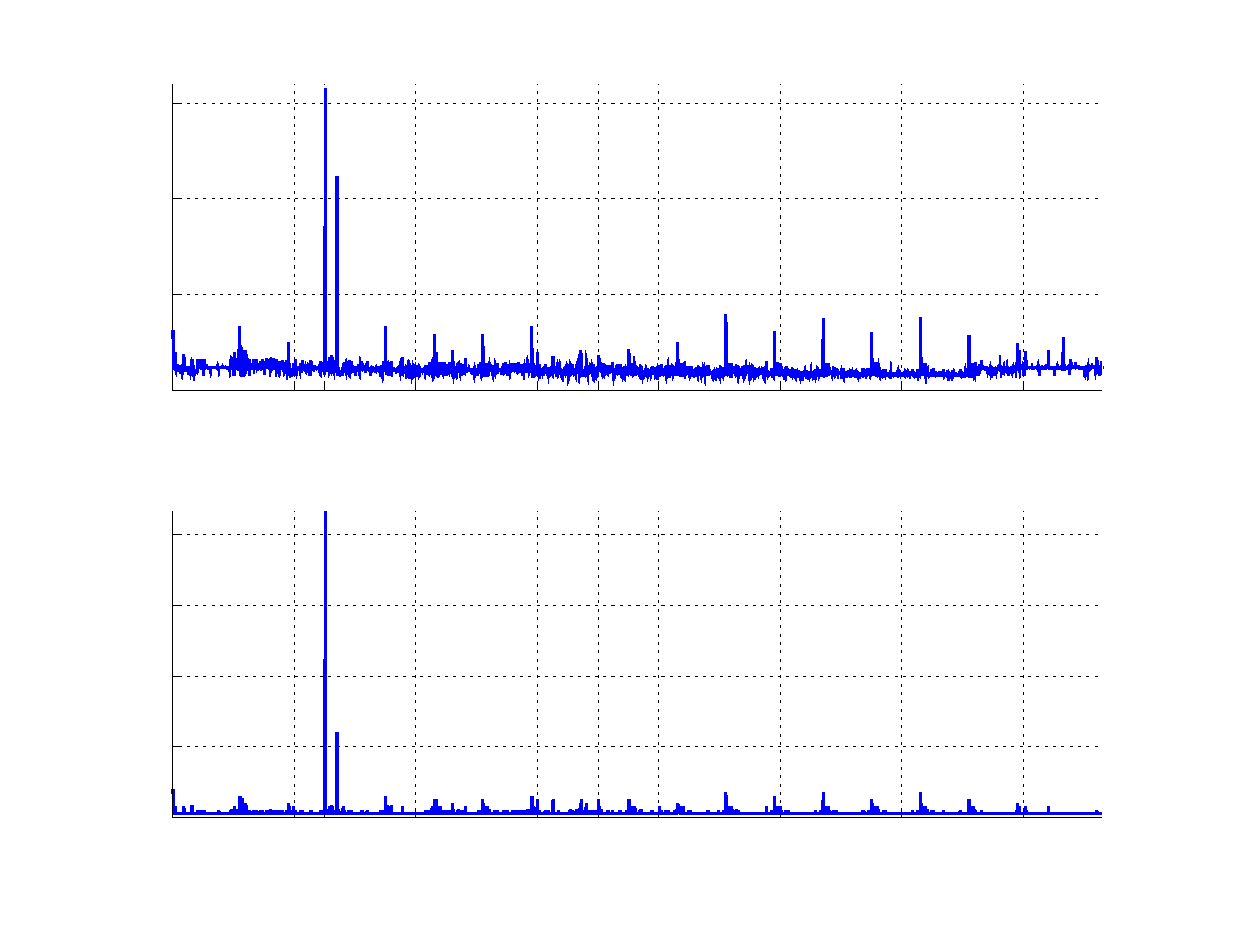
\includegraphics[trim=30  20   0   0,clip,scale=0.42]{time_16_02_01_N16-inc}
\end{picture}%
\begin{picture}(546, 412)(30,20)
\fontsize{8}{0}
\selectfont\put(74.88,247.205){\makebox(0,0)[t]{\textcolor[rgb]{0,0,0}{{0}}}}
\fontsize{8}{0}
\selectfont\put(133.214,247.205){\makebox(0,0)[t]{\textcolor[rgb]{0,0,0}{{2}}}}
\fontsize{8}{0}
\selectfont\put(147.797,247.205){\makebox(0,0)[t]{\textcolor[rgb]{0,0,0}{{$~\impulseC_d^y$}}}}
\fontsize{8}{0}
\selectfont\put(191.548,247.205){\makebox(0,0)[t]{\textcolor[rgb]{0,0,0}{{4}}}}
\fontsize{8}{0}
\selectfont\put(249.882,247.205){\makebox(0,0)[t]{\textcolor[rgb]{0,0,0}{{6}}}}
\fontsize{8}{0}
\selectfont\put(279.049,247.205){\makebox(0,0)[t]{\textcolor[rgb]{0,0,0}{{$\impulseC_d^x$}}}}
\fontsize{8}{0}
\selectfont\put(308.216,247.205){\makebox(0,0)[t]{\textcolor[rgb]{0,0,0}{{8}}}}
\fontsize{8}{0}
\selectfont\put(366.549,247.205){\makebox(0,0)[t]{\textcolor[rgb]{0,0,0}{{10}}}}
\fontsize{8}{0}
\selectfont\put(424.883,247.205){\makebox(0,0)[t]{\textcolor[rgb]{0,0,0}{{12}}}}
\fontsize{8}{0}
\selectfont\put(483.217,247.205){\makebox(0,0)[t]{\textcolor[rgb]{0,0,0}{{14}}}}
\fontsize{8}{0}
\selectfont\put(69.8755,252.218){\makebox(0,0)[r]{\textcolor[rgb]{0,0,0}{{0}}}}
\fontsize{8}{0}
\selectfont\put(69.8755,298.275){\makebox(0,0)[r]{\textcolor[rgb]{0,0,0}{{5}}}}
\fontsize{8}{0}
\selectfont\put(69.8755,344.332){\makebox(0,0)[r]{\textcolor[rgb]{0,0,0}{{10}}}}
\fontsize{8}{0}
\selectfont\put(69.8755,390.389){\makebox(0,0)[r]{\textcolor[rgb]{0,0,0}{{15}}}}
\fontsize{8}{0}
\selectfont\put(31.8755,325.909){\rotatebox{90}{\makebox(0,0)[t]{\textcolor[rgb]{0,0,0}{{comp. time $[ms]$}}}}}
\fontsize{8}{0}
\selectfont\put(74.88,42.507){\makebox(0,0)[t]{\textcolor[rgb]{0,0,0}{{0}}}}
\fontsize{8}{0}
\selectfont\put(133.214,42.507){\makebox(0,0)[t]{\textcolor[rgb]{0,0,0}{{2}}}}
\fontsize{8}{0}
\selectfont\put(147.797,42.507){\makebox(0,0)[t]{\textcolor[rgb]{0,0,0}{{$~\impulseC_d^y$}}}}
\fontsize{8}{0}
\selectfont\put(191.548,42.507){\makebox(0,0)[t]{\textcolor[rgb]{0,0,0}{{4}}}}
\fontsize{8}{0}
\selectfont\put(249.882,42.507){\makebox(0,0)[t]{\textcolor[rgb]{0,0,0}{{6}}}}
\fontsize{8}{0}
\selectfont\put(279.049,42.507){\makebox(0,0)[t]{\textcolor[rgb]{0,0,0}{{$\impulseC_d^x$}}}}
\fontsize{8}{0}
\selectfont\put(308.216,42.507){\makebox(0,0)[t]{\textcolor[rgb]{0,0,0}{{8}}}}
\fontsize{8}{0}
\selectfont\put(366.549,42.507){\makebox(0,0)[t]{\textcolor[rgb]{0,0,0}{{10}}}}
\fontsize{8}{0}
\selectfont\put(424.883,42.507){\makebox(0,0)[t]{\textcolor[rgb]{0,0,0}{{12}}}}
\fontsize{8}{0}
\selectfont\put(483.217,42.507){\makebox(0,0)[t]{\textcolor[rgb]{0,0,0}{{14}}}}
\fontsize{8}{0}
\selectfont\put(69.8755,47.52){\makebox(0,0)[r]{\textcolor[rgb]{0,0,0}{{0}}}}
\fontsize{8}{0}
\selectfont\put(69.8755,81.401){\makebox(0,0)[r]{\textcolor[rgb]{0,0,0}{{20}}}}
\fontsize{8}{0}
\selectfont\put(69.8755,115.282){\makebox(0,0)[r]{\textcolor[rgb]{0,0,0}{{40}}}}
\fontsize{8}{0}
\selectfont\put(69.8755,149.163){\makebox(0,0)[r]{\textcolor[rgb]{0,0,0}{{60}}}}
\fontsize{8}{0}
\selectfont\put(69.8755,183.044){\makebox(0,0)[r]{\textcolor[rgb]{0,0,0}{{80}}}}
\fontsize{8}{0}
\selectfont\put(298.08,9.50697){\makebox(0,0)[t]{\textcolor[rgb]{0,0,0}{{simulation time $[s]$}}}}
\fontsize{8}{0}
\selectfont\put(31.8755,121.211){\rotatebox{90}{\makebox(0,0)[t]{\textcolor[rgb]{0,0,0}{{num. of iterations}}}}}
\end{picture}

            \subcaption{
                $N = 16$, with disturbances.\\
                Mean computational time: $1.09~[\MT{ms}]$.\\
                Time measurements $> 1~[\MT{ms}]$: 62\%
            }
            \label{fig.task_walk_time.2}
        }
    \end{minipage}
    \begin{minipage}[t]{0.49\textwidth}
        \centering{
            % Title: glps_renderer figure
% Creator: GL2PS 1.3.8, (C) 1999-2012 C. Geuzaine
% For: Octave
% CreationDate: Wed Mar 23 19:36:51 2016
\setlength{\unitlength}{0.42pt}
\begin{picture}(0,0)
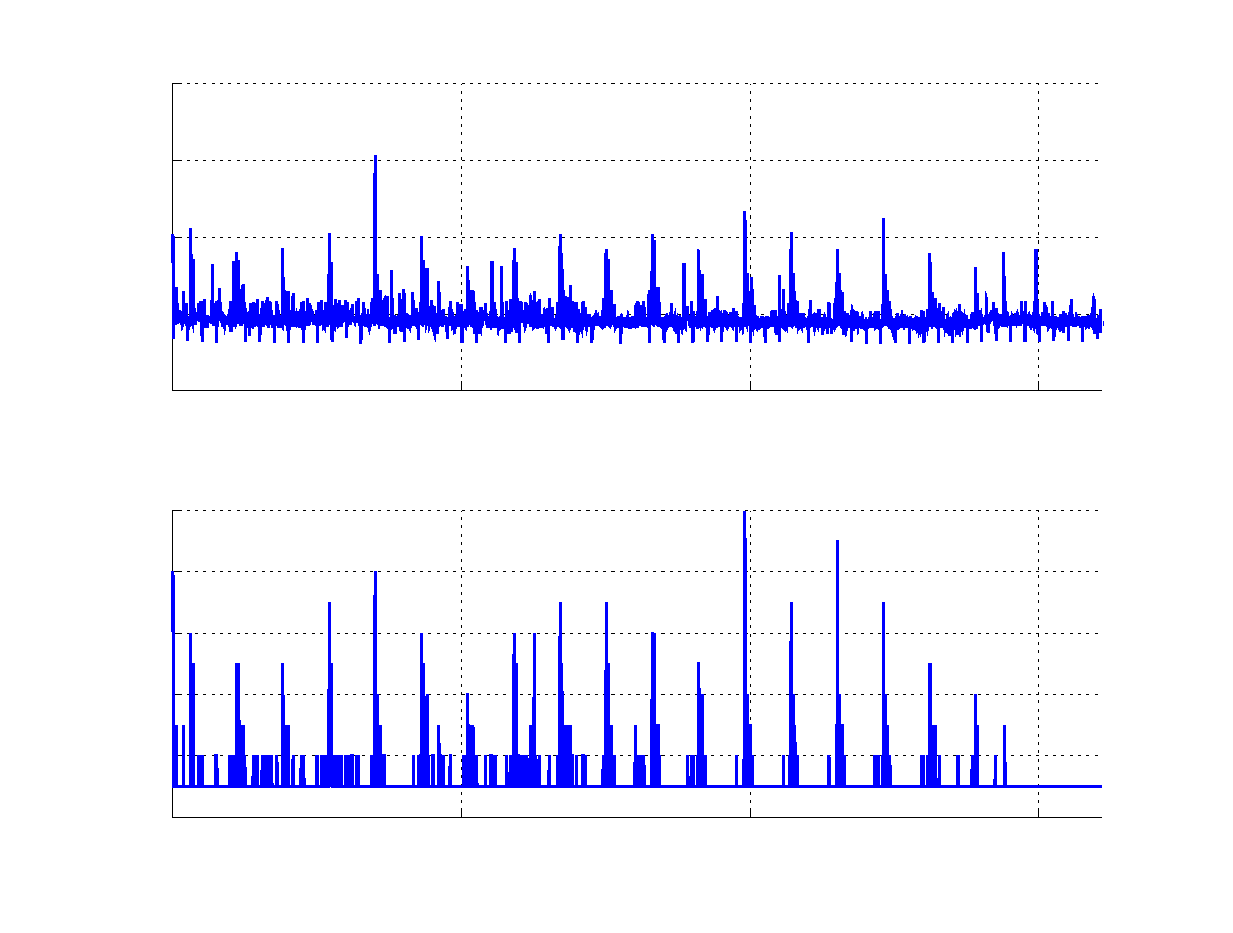
\includegraphics[trim=30  20   0   0,clip,scale=0.42]{time_16_02_04_N8_nodist-inc}
\end{picture}%
\begin{picture}(546, 412)(30,20)
\fontsize{8}{0}
\selectfont\put(74.88,247.205){\makebox(0,0)[t]{\textcolor[rgb]{0,0,0}{{0}}}}
\fontsize{8}{0}
\selectfont\put(213.47,247.205){\makebox(0,0)[t]{\textcolor[rgb]{0,0,0}{{5}}}}
\fontsize{8}{0}
\selectfont\put(352.061,247.205){\makebox(0,0)[t]{\textcolor[rgb]{0,0,0}{{10}}}}
\fontsize{8}{0}
\selectfont\put(490.651,247.205){\makebox(0,0)[t]{\textcolor[rgb]{0,0,0}{{15}}}}
\fontsize{8}{0}
\selectfont\put(69.8755,252.218){\makebox(0,0)[r]{\textcolor[rgb]{0,0,0}{{0}}}}
\fontsize{8}{0}
\selectfont\put(69.8755,289.063){\makebox(0,0)[r]{\textcolor[rgb]{0,0,0}{{1}}}}
\fontsize{8}{0}
\selectfont\put(69.8755,325.909){\makebox(0,0)[r]{\textcolor[rgb]{0,0,0}{{2}}}}
\fontsize{8}{0}
\selectfont\put(69.8755,362.754){\makebox(0,0)[r]{\textcolor[rgb]{0,0,0}{{3}}}}
\fontsize{8}{0}
\selectfont\put(69.8755,399.6){\makebox(0,0)[r]{\textcolor[rgb]{0,0,0}{{4}}}}
\fontsize{8}{0}
\selectfont\put(48.8755,325.909){\rotatebox{90}{\makebox(0,0)[b]{\textcolor[rgb]{0,0,0}{{comp. time $[ms]$}}}}}
\fontsize{8}{0}
\selectfont\put(74.88,42.507){\makebox(0,0)[t]{\textcolor[rgb]{0,0,0}{{0}}}}
\fontsize{8}{0}
\selectfont\put(213.47,42.507){\makebox(0,0)[t]{\textcolor[rgb]{0,0,0}{{5}}}}
\fontsize{8}{0}
\selectfont\put(352.061,42.507){\makebox(0,0)[t]{\textcolor[rgb]{0,0,0}{{10}}}}
\fontsize{8}{0}
\selectfont\put(490.651,42.507){\makebox(0,0)[t]{\textcolor[rgb]{0,0,0}{{15}}}}
\fontsize{8}{0}
\selectfont\put(69.8755,47.52){\makebox(0,0)[r]{\textcolor[rgb]{0,0,0}{{0}}}}
\fontsize{8}{0}
\selectfont\put(69.8755,76.9964){\makebox(0,0)[r]{\textcolor[rgb]{0,0,0}{{2}}}}
\fontsize{8}{0}
\selectfont\put(69.8755,106.473){\makebox(0,0)[r]{\textcolor[rgb]{0,0,0}{{4}}}}
\fontsize{8}{0}
\selectfont\put(69.8755,135.949){\makebox(0,0)[r]{\textcolor[rgb]{0,0,0}{{6}}}}
\fontsize{8}{0}
\selectfont\put(69.8755,165.426){\makebox(0,0)[r]{\textcolor[rgb]{0,0,0}{{8}}}}
\fontsize{8}{0}
\selectfont\put(69.8755,194.902){\makebox(0,0)[r]{\textcolor[rgb]{0,0,0}{{10}}}}
\fontsize{8}{0}
\selectfont\put(298.08,9.50697){\makebox(0,0)[t]{\textcolor[rgb]{0,0,0}{{simulation time $[s]$}}}}
\fontsize{8}{0}
\selectfont\put(31.8755,121.211){\rotatebox{90}{\makebox(0,0)[t]{\textcolor[rgb]{0,0,0}{{num. of iterations}}}}}
\end{picture}

            \subcaption{
                $N = 8$, without disturbances.\\
                Mean computational time: $9.4~[\MT{ms}]$.\\
                Time measurements $> 1~[\MT{ms}]$: 11\%
            }
            \label{fig.task_walk_time.3}
        }
    \end{minipage}
    \hfill
    \begin{minipage}[t]{0.49\textwidth}
        \centering{
            % Title: glps_renderer figure
% Creator: GL2PS 1.3.8, (C) 1999-2012 C. Geuzaine
% For: Octave
% CreationDate: Wed Mar 23 19:36:50 2016
\setlength{\unitlength}{0.42pt}
\begin{picture}(0,0)
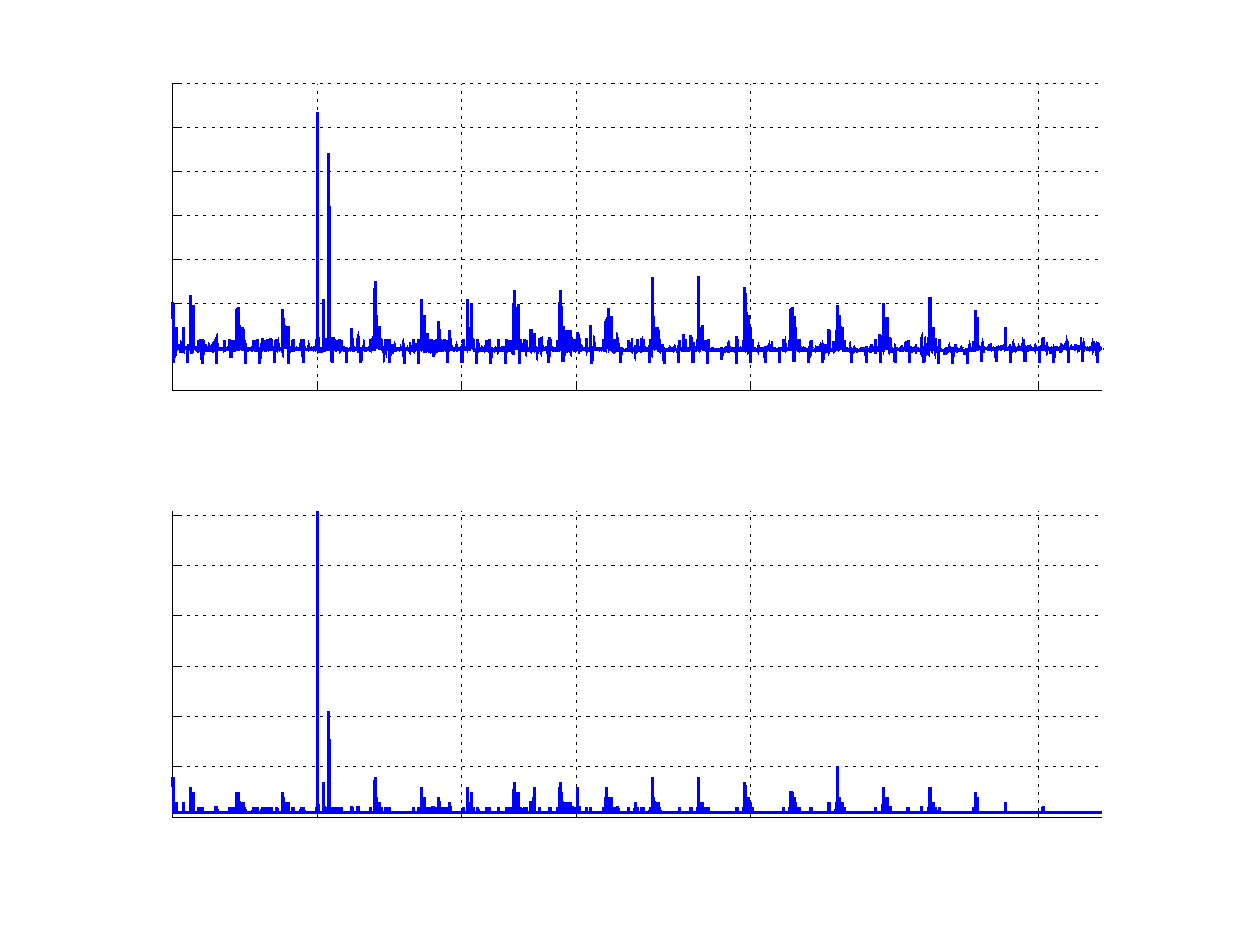
\includegraphics[trim=30  20   0   0,clip,scale=0.42]{time_16_02_02_N8-inc}
\end{picture}%
\begin{picture}(546, 412)(30,20)
\fontsize{8}{0}
\selectfont\put(74.88,247.205){\makebox(0,0)[t]{\textcolor[rgb]{0,0,0}{{0}}}}
\fontsize{8}{0}
\selectfont\put(144.175,247.205){\makebox(0,0)[t]{\textcolor[rgb]{0,0,0}{{$\impulseC_d^y$}}}}
\fontsize{8}{0}
\selectfont\put(213.47,247.205){\makebox(0,0)[t]{\textcolor[rgb]{0,0,0}{{5}}}}
\fontsize{8}{0}
\selectfont\put(268.907,247.205){\makebox(0,0)[t]{\textcolor[rgb]{0,0,0}{{$\impulseC_d^x$}}}}
\fontsize{8}{0}
\selectfont\put(352.061,247.205){\makebox(0,0)[t]{\textcolor[rgb]{0,0,0}{{10}}}}
\fontsize{8}{0}
\selectfont\put(490.651,247.205){\makebox(0,0)[t]{\textcolor[rgb]{0,0,0}{{15}}}}
\fontsize{8}{0}
\selectfont\put(69.8755,252.218){\makebox(0,0)[r]{\textcolor[rgb]{0,0,0}{{0}}}}
\fontsize{8}{0}
\selectfont\put(69.8755,273.272){\makebox(0,0)[r]{\textcolor[rgb]{0,0,0}{{1}}}}
\fontsize{8}{0}
\selectfont\put(69.8755,294.327){\makebox(0,0)[r]{\textcolor[rgb]{0,0,0}{{2}}}}
\fontsize{8}{0}
\selectfont\put(69.8755,315.382){\makebox(0,0)[r]{\textcolor[rgb]{0,0,0}{{3}}}}
\fontsize{8}{0}
\selectfont\put(69.8755,336.436){\makebox(0,0)[r]{\textcolor[rgb]{0,0,0}{{4}}}}
\fontsize{8}{0}
\selectfont\put(69.8755,357.491){\makebox(0,0)[r]{\textcolor[rgb]{0,0,0}{{5}}}}
\fontsize{8}{0}
\selectfont\put(69.8755,378.545){\makebox(0,0)[r]{\textcolor[rgb]{0,0,0}{{6}}}}
\fontsize{8}{0}
\selectfont\put(69.8755,399.6){\makebox(0,0)[r]{\textcolor[rgb]{0,0,0}{{7}}}}
\fontsize{8}{0}
\selectfont\put(48.8755,325.909){\rotatebox{90}{\makebox(0,0)[b]{\textcolor[rgb]{0,0,0}{{comp. time $[ms]$}}}}}
\fontsize{8}{0}
\selectfont\put(74.88,42.507){\makebox(0,0)[t]{\textcolor[rgb]{0,0,0}{{0}}}}
\fontsize{8}{0}
\selectfont\put(144.175,42.507){\makebox(0,0)[t]{\textcolor[rgb]{0,0,0}{{$\impulseC_d^y$}}}}
\fontsize{8}{0}
\selectfont\put(213.47,42.507){\makebox(0,0)[t]{\textcolor[rgb]{0,0,0}{{5}}}}
\fontsize{8}{0}
\selectfont\put(268.907,42.507){\makebox(0,0)[t]{\textcolor[rgb]{0,0,0}{{$\impulseC_d^x$}}}}
\fontsize{8}{0}
\selectfont\put(352.061,42.507){\makebox(0,0)[t]{\textcolor[rgb]{0,0,0}{{10}}}}
\fontsize{8}{0}
\selectfont\put(490.651,42.507){\makebox(0,0)[t]{\textcolor[rgb]{0,0,0}{{15}}}}
\fontsize{8}{0}
\selectfont\put(69.8755,47.52){\makebox(0,0)[r]{\textcolor[rgb]{0,0,0}{{0}}}}
\fontsize{8}{0}
\selectfont\put(69.8755,71.681){\makebox(0,0)[r]{\textcolor[rgb]{0,0,0}{{10}}}}
\fontsize{8}{0}
\selectfont\put(69.8755,95.842){\makebox(0,0)[r]{\textcolor[rgb]{0,0,0}{{20}}}}
\fontsize{8}{0}
\selectfont\put(69.8755,120.003){\makebox(0,0)[r]{\textcolor[rgb]{0,0,0}{{30}}}}
\fontsize{8}{0}
\selectfont\put(69.8755,144.164){\makebox(0,0)[r]{\textcolor[rgb]{0,0,0}{{40}}}}
\fontsize{8}{0}
\selectfont\put(69.8755,168.325){\makebox(0,0)[r]{\textcolor[rgb]{0,0,0}{{50}}}}
\fontsize{8}{0}
\selectfont\put(69.8755,192.486){\makebox(0,0)[r]{\textcolor[rgb]{0,0,0}{{60}}}}
\fontsize{8}{0}
\selectfont\put(298.08,9.50697){\makebox(0,0)[t]{\textcolor[rgb]{0,0,0}{{simulation time $[s]$}}}}
\fontsize{8}{0}
\selectfont\put(31.8755,121.211){\rotatebox{90}{\makebox(0,0)[b]{\textcolor[rgb]{0,0,0}{{num. of iterations}}}}}
\end{picture}

            \subcaption{
                $N = 8$, with disturbances.\\
                Mean computational time: $9.8~[\MT{ms}]$.\\
                Time measurements $> 1~[\MT{ms}]$: 13\%
            }
            \label{fig.task_walk_time.4}
        }
    \end{minipage}
    \caption[Computation time and number of iterations of \sn{LexLS}.]{
        Computation time and number of iterations of \sn{LexLS}. Time instants,
        when disturbances are applied, are indicated with $\impulseC_d^y$ and
        $\impulseC_d^x$.
    }
    \label{fig.task_walk_time}
\end{figure*}


\cref{hr.mmpc_walk} is supposed to be solved in order of milliseconds to
control a robot in real time. This is a challenging problem, since the
hierarchy has around $85$ decision variables and includes more than $100$
inequality and $120$ equality constraints. In order to demonstrate that this is
possible we measured the time required for \sn{LexLS} to solve this \ac{PLLS}
problem (see \cref{fig.task_walk_time.1,fig.task_walk_time.2}). The time
measurement at each control instant is averaged over three simulation runs to
suppress outliers. All measurements were performed on a laptop with Intel Core
i5-3360M ($2.80~[\MT{GHz}]$) \acs{CPU}.


When disturbances are not applied, the time required to solve the hierarchy is
less than $5~[\MT{ms}]$, the number of iterations of the solver does not exceed
$8$. However, disturbances lead to increase in the number of iterations of the
solver, which, in turn, leads to significant increase in the computational
time. In order to alleviate this issue it might be necessary to employ early
termination of the solver (see \cref{sec.early_termination}). It is, however,
important to note, that the current implementation of \sn{LexLS} adds and
removes constraints from the active set in an inefficient way
\cite{Dimitrov2015preprint}. Hence, further development of the solver is
expected to give a performance boost for the controller. In an attempt to
reduce the computational time, we also tried to shorten the preview horizon
from $N = 16$ to $N = 8$ sampling intervals. This modification reduces the
number of decision variables by $16$-$18$, the number of equality and
inequality constraints by $32$ and $16$-$18$ respectively. The problem with
shorter preview horizon can be solved slightly faster on average and 2 times
faster, when disturbance is applied (see
\cref{fig.task_walk_time.3,fig.task_walk_time.4}). One can also observe that in
almost $90$\% of the cases the problem is solved faster than $1~[\MT{ms}]$. At
the same time, we did not observe qualitative changes in behavior of the robot.



%%%%%%%%%%%%%%%%%%%%%%%%%%%%%%%%%%%%%%%%%%%%%%%%%%%%%%%%%%%%%%%%%%%%%%%%%%%%%%%%
\subsubsection{Quality of the motion}\label{sec.motion_quality}

Although, the controller produces the desired behavior, the generated motion is
not completely satisfactory:
%
\begin{itemize}
    \item \cref{fig.task_walk_x,fig.task_walk_y} demonstrate that the right
        hand position oscillates near the target in the end of the simulation
        due to the sway motion of the robot. This may be caused by several
        reasons: ({\bf i}) compromise between satisfaction of the hand task and
        other tasks on the last level of the hierarchy, ({\bf ii}) lack of
        anticipation for the hand position and respective kinematic
        constraints.

    \item We can see in \cref{fig.task_walk_steps_time_x_magnified} (as well as
        in \cref{fig.task_walk_steps_time_x,fig.task_walk_steps_time_y})
        periodic variations of the \ac{CoP} position with period of
        $0.1~[\MT{s}]$ caused by the discrepancy between the control interval
        of $0.005~[\MT{s}]$ and preview sampling interval of $0.1~[\MT{s}]$.
        This issue was discussed in \cref{sec.sampling_interval}.

\begin{figure}[!htbp]
    \centering{
        % Title: glps_renderer figure
% Creator: GL2PS 1.3.8, (C) 1999-2012 C. Geuzaine
% For: Octave
% CreationDate: Wed Mar 30 19:27:51 2016
\setlength{\unitlength}{0.7pt}
\begin{picture}(0,0)
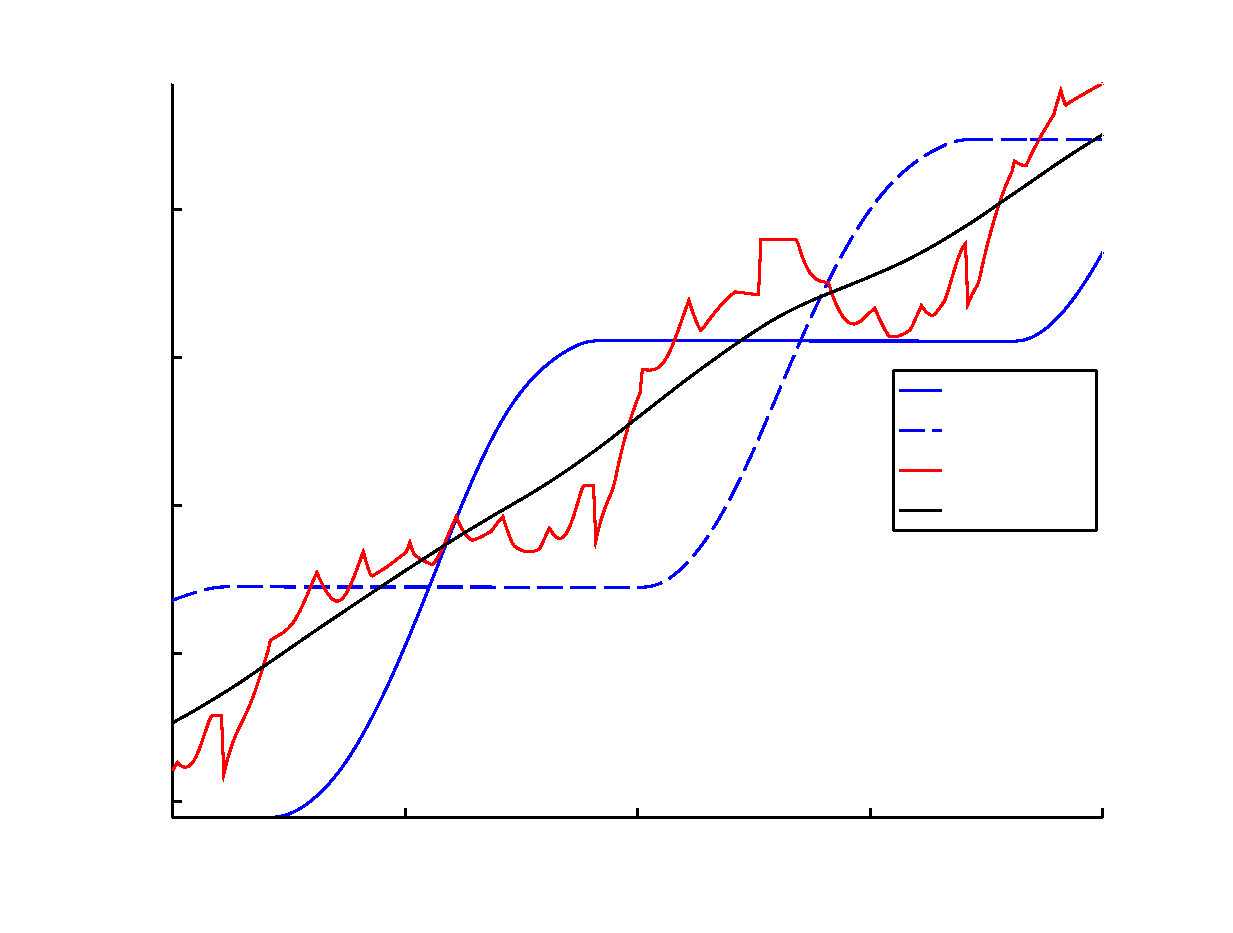
\includegraphics[trim=50   0  50  10,clip,scale=0.7]{steps_time_x_16_02_01_N16_nodist_magnified-inc}
\end{picture}%
\begin{picture}(476, 422)(50,0)
\fontsize{11}{0}
\selectfont\put(74.88,42.5188){\makebox(0,0)[t]{\textcolor[rgb]{0,0,0}{{5}}}}
\fontsize{11}{0}
\selectfont\put(186.48,42.5188){\makebox(0,0)[t]{\textcolor[rgb]{0,0,0}{{5.5}}}}
\fontsize{11}{0}
\selectfont\put(298.08,42.5188){\makebox(0,0)[t]{\textcolor[rgb]{0,0,0}{{6}}}}
\fontsize{11}{0}
\selectfont\put(409.68,42.5188){\makebox(0,0)[t]{\textcolor[rgb]{0,0,0}{{6.5}}}}
\fontsize{11}{0}
\selectfont\put(521.28,42.5188){\makebox(0,0)[t]{\textcolor[rgb]{0,0,0}{{7}}}}
\fontsize{11}{0}
\selectfont\put(69.8755,54.9812){\makebox(0,0)[r]{\textcolor[rgb]{0,0,0}{{0.6}}}}
\fontsize{11}{0}
\selectfont\put(69.8755,126.071){\makebox(0,0)[r]{\textcolor[rgb]{0,0,0}{{0.7}}}}
\fontsize{11}{0}
\selectfont\put(69.8755,197.161){\makebox(0,0)[r]{\textcolor[rgb]{0,0,0}{{0.8}}}}
\fontsize{11}{0}
\selectfont\put(69.8755,268.25){\makebox(0,0)[r]{\textcolor[rgb]{0,0,0}{{0.9}}}}
\fontsize{11}{0}
\selectfont\put(69.8755,339.34){\makebox(0,0)[r]{\textcolor[rgb]{0,0,0}{{1}}}}
\fontsize{11}{0}
\selectfont\put(298.08,22.5188){\makebox(0,0)[t]{\textcolor[rgb]{0,0,0}{{simulation time $[s]$}}}}
\fontsize{11}{0}
\selectfont\put(40.8755,223.56){\rotatebox{90}{\makebox(0,0)[b]{\textcolor[rgb]{0,0,0}{{position along the $x$ axis $[m]$}}}}}
\fontsize{11}{0}
\selectfont\put(446.874,252.364){\makebox(0,0)[l]{\textcolor[rgb]{0,0,0}{{Left foot}}}}
\fontsize{11}{0}
\selectfont\put(446.874,233.161){\makebox(0,0)[l]{\textcolor[rgb]{0,0,0}{{Right foot}}}}
\fontsize{11}{0}
\selectfont\put(446.874,213.959){\makebox(0,0)[l]{\textcolor[rgb]{0,0,0}{{CoP}}}}
\fontsize{11}{0}
\selectfont\put(446.874,194.756){\makebox(0,0)[l]{\textcolor[rgb]{0,0,0}{{CoM}}}}
\end{picture}

        \caption[Periodic variations in the CoP position.]{
            Magnified part of \cref{fig.task_walk_steps_time_x.nodist}:
            evolution of the feet, \ac{CoM}, and \ac{CoP} positions with time
            along the $x$ axis. Periodic variations of the \ac{CoP} position
            with period $0.1~[\MT{s}]$ can be clearly seen.
        }
        \label{fig.task_walk_steps_time_x_magnified}
    }
\end{figure}

    \item The controller is designed in such a way, that it always trades off
        between two strategies for reaching the target: moving the hand and
        walking. Consequently, near singularities of the elbow, the controller
        prefers walking to bending the arm, which is undesirable in some
        situations.

    \item We tuned the weights on the last level of the hierarchy so that the
        \ac{CoP} centering task dominates all others. The reason for this is
        that the hand task ``pulls'' the \ac{CoP} to the front edges of the
        support areas, which, to some extend, corresponds to walking on
        tiptoes. This negatively impacts controller's ability to cope with
        disturbances and, therefore, is potentially unsafe
        \cite{Lafaye2014humanoids}. Moreover, it leads to a larger number of
        active inequality constraints and larger number of iterations of the
        solver.
\end{itemize}



%%%%%%%%%%%%%%%%%%%%%%%%%%%%%%%%%%%%%%%%%%%%%%%%%%%%%%%%%%%%%%%%%%%%%%%%%%%%%%%%
\subsection{Conclusion}\label{sec.task_walk_conclusion}

We demonstrated that \ac{MMPC} allows to account for the whole body tasks while
generating walking motions without relying on time-demanding planning and
nonlinear optimization procedures \cite{Escande2009iros, Kanoun2010ijrr,
Tassa2014icra}. The major limitation of the approach is the fact that durations
and sequence of the steps must still be decided outside of the controller.
There is also a number of technical difficulties discussed in
\cref{sec.motion_quality}, which should be addressed in the future works.


\FloatBarrier



%%%%%%%%%%%%%%%%%%%%%%%%%%%%%%%%%%%%%%%%%%%%%%%%%%%%%%%%%%%%%%%%%%%%%%%%%%%%%%%%
%%%%%%%%%%%%%%%%%%%%%%%%%%%%%%%%%%%%%%%%%%%%%%%%%%%%%%%%%%%%%%%%%%%%%%%%%%%%%%%%
%%%%%%%%%%%%%%%%%%%%%%%%%%%%%%%%%%%%%%%%%%%%%%%%%%%%%%%%%%%%%%%%%%%%%%%%%%%%%%%%
\section{Prioritization in the contact force distribution}\label{sec.optional_force}

We continued to develop the idea of \ac{MMPC} in \cite{Sherikov2015humanoids},
where we proposed a controller for balancing in a multicontact setting with
prioritized contact force distribution. In most settings with multiple contacts
there exists an infinite number of force distributions that achieve the same
base motion. The typical approach to resolve this ambiguity is to make contacts
as robust as possible, by keeping each contact force far from the bounds of the
respective friction cone, and distribute the forces evenly between all the
contacts~\cite{Saab2013tro, Ott2011humanoids, Herzog2015auro, Hyon2007tro}.
There are situations, however, such as when a contact area is fragile, when it
is preferable to avoid using it unless strictly necessary for balance. In this
case, distributing forces evenly between all possible contacts should be
avoided. We propose therefore to introduce a prioritized distribution of the
contact forces, with the help of hierarchical optimization~\cite{Saab2013tro,
Escande2014ijrr, Kanoun2011tro}. We demonstrate our idea in a setting, where a
humanoid robot can optionally exploit a hand contact with an additional support
to maintain balance and execute certain task with the free hand.



%%%%%%%%%%%%%%%%%%%%%%%%%%%%%%%%%%%%%%%%%%%%%%%%%%%%%%%%%%%%%%%%%%%%%%%%%%%%%%%%
\subsection{Setting}\label{sec.force_setting}

\begin{figure}[!htb]
    \begin{minipage}[t]{0.49\textwidth}
        \centering{
            % Title: glps_renderer figure
% Creator: GL2PS 1.3.8, (C) 1999-2012 C. Geuzaine
% For: Octave
% CreationDate: Mon May  9 19:27:08 2016
\setlength{\unitlength}{0.42pt}
\begin{picture}(0,0)
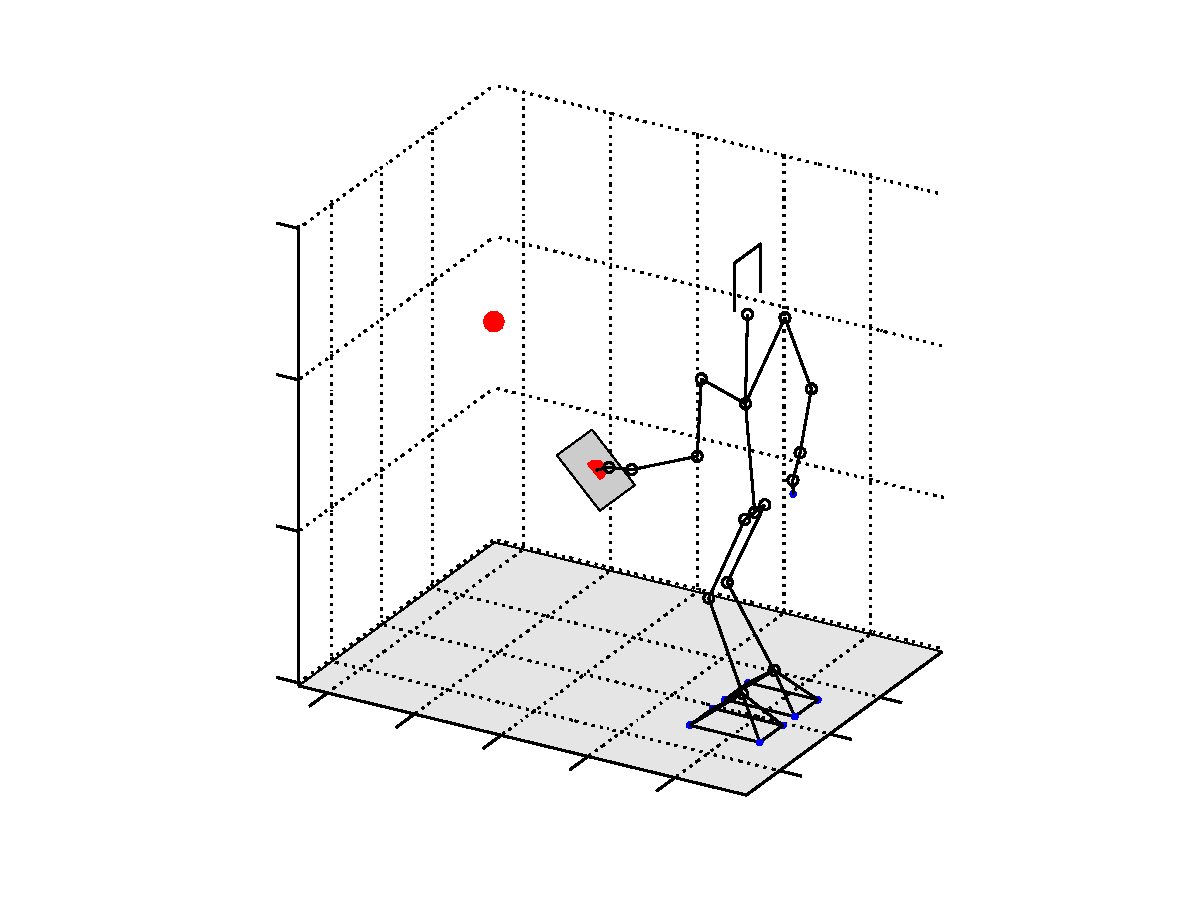
\includegraphics[trim=50  46  50   0,clip,scale=0.42]{test_17_23_robot_1-inc}
\end{picture}%
\begin{picture}(460, 374)(50,46)
\fontsize{7}{0}
\selectfont\put(119.905,103.852){\makebox(0,0)[br]{\textcolor[rgb]{0,0,0}{{0}}}}
\fontsize{7}{0}
\selectfont\put(119.905,176.551){\makebox(0,0)[br]{\textcolor[rgb]{0,0,0}{{0.5}}}}
\fontsize{7}{0}
\selectfont\put(119.905,249.249){\makebox(0,0)[br]{\textcolor[rgb]{0,0,0}{{1}}}}
\fontsize{7}{0}
\selectfont\put(119.905,321.947){\makebox(0,0)[br]{\textcolor[rgb]{0,0,0}{{1.5}}}}
\fontsize{7}{0}
\selectfont\put(429.718,89.3565){\makebox(0,0)[tl]{\textcolor[rgb]{0,0,0}{{-0.3}}}}
\fontsize{7}{0}
\selectfont\put(136.413,85.8912){\makebox(0,0)[tr]{\textcolor[rgb]{0,0,0}{{1.2}}}}
\fontsize{7}{0}
\selectfont\put(178.093,75.7213){\makebox(0,0)[tr]{\textcolor[rgb]{0,0,0}{{0.9}}}}
\fontsize{7}{0}
\selectfont\put(405.654,71.7417){\makebox(0,0)[tl]{\textcolor[rgb]{0,0,0}{{0}}}}
\fontsize{7}{0}
\selectfont\put(219.773,65.5514){\makebox(0,0)[tr]{\textcolor[rgb]{0,0,0}{{0.6}}}}
\fontsize{7}{0}
\selectfont\put(261.453,55.3814){\makebox(0,0)[tr]{\textcolor[rgb]{0,0,0}{{0.3}}}}
\fontsize{7}{0}
\selectfont\put(303.133,45.2115){\makebox(0,0)[tr]{\textcolor[rgb]{0,0,0}{{0}}}}
\fontsize{7}{0}
\selectfont\put(381.59,54.1268){\makebox(0,0)[tl]{\textcolor[rgb]{0,0,0}{{0.3}}}}
\end{picture}

            \subcaption{initial configuration}
            \label{fig.force_distrib.1}
        }
    \end{minipage}
    \hfill
    \begin{minipage}[t]{0.49\textwidth}
        \centering{
            % Title: glps_renderer figure
% Creator: GL2PS 1.3.8, (C) 1999-2012 C. Geuzaine
% For: Octave
% CreationDate: Mon May  9 19:27:09 2016
\setlength{\unitlength}{0.42pt}
\begin{picture}(0,0)
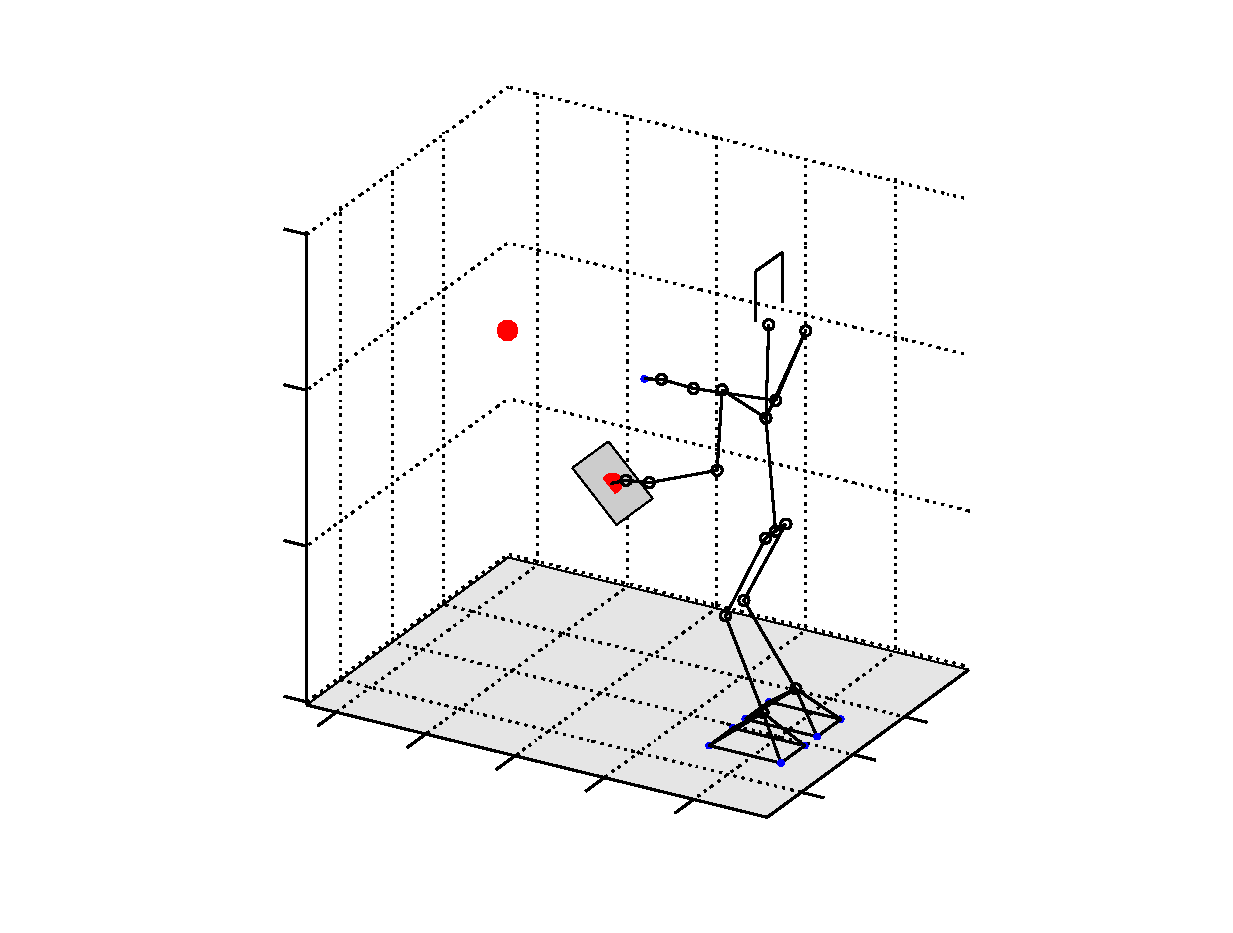
\includegraphics[trim=50  46  50   0,clip,scale=0.42]{test_17_23_robot_1001-inc}
\end{picture}%
\begin{picture}(476, 386)(50,46)
\fontsize{7}{0}
\selectfont\put(123.469,106.786){\makebox(0,0)[br]{\textcolor[rgb]{0,0,0}{{0}}}}
\fontsize{7}{0}
\selectfont\put(123.469,181.561){\makebox(0,0)[br]{\textcolor[rgb]{0,0,0}{{0.5}}}}
\fontsize{7}{0}
\selectfont\put(123.469,256.337){\makebox(0,0)[br]{\textcolor[rgb]{0,0,0}{{1}}}}
\fontsize{7}{0}
\selectfont\put(123.469,331.112){\makebox(0,0)[br]{\textcolor[rgb]{0,0,0}{{1.5}}}}
\fontsize{7}{0}
\selectfont\put(140.455,88.4511){\makebox(0,0)[tr]{\textcolor[rgb]{0,0,0}{{1.2}}}}
\fontsize{7}{0}
\selectfont\put(183.326,77.9906){\makebox(0,0)[tr]{\textcolor[rgb]{0,0,0}{{0.9}}}}
\fontsize{7}{0}
\selectfont\put(226.197,67.5301){\makebox(0,0)[tr]{\textcolor[rgb]{0,0,0}{{0.6}}}}
\fontsize{7}{0}
\selectfont\put(269.068,57.0696){\makebox(0,0)[tr]{\textcolor[rgb]{0,0,0}{{0.3}}}}
\fontsize{7}{0}
\selectfont\put(311.939,46.6091){\makebox(0,0)[tr]{\textcolor[rgb]{0,0,0}{{0}}}}
\fontsize{7}{0}
\selectfont\put(441.858,91.9431){\makebox(0,0)[tl]{\textcolor[rgb]{0,0,0}{{-0.3}}}}
\fontsize{7}{0}
\selectfont\put(417.107,73.825){\makebox(0,0)[tl]{\textcolor[rgb]{0,0,0}{{0}}}}
\fontsize{7}{0}
\selectfont\put(392.355,55.7069){\makebox(0,0)[tl]{\textcolor[rgb]{0,0,0}{{0.3}}}}
\end{picture}

            \subcaption{after $5$ seconds}
            \label{fig.force_distrib.2}
        }
    \end{minipage}
    \begin{minipage}[t]{0.49\textwidth}
        \centering{
            % Title: glps_renderer figure
% Creator: GL2PS 1.3.8, (C) 1999-2012 C. Geuzaine
% For: Octave
% CreationDate: Mon May  9 19:27:11 2016
\setlength{\unitlength}{0.42pt}
\begin{picture}(0,0)
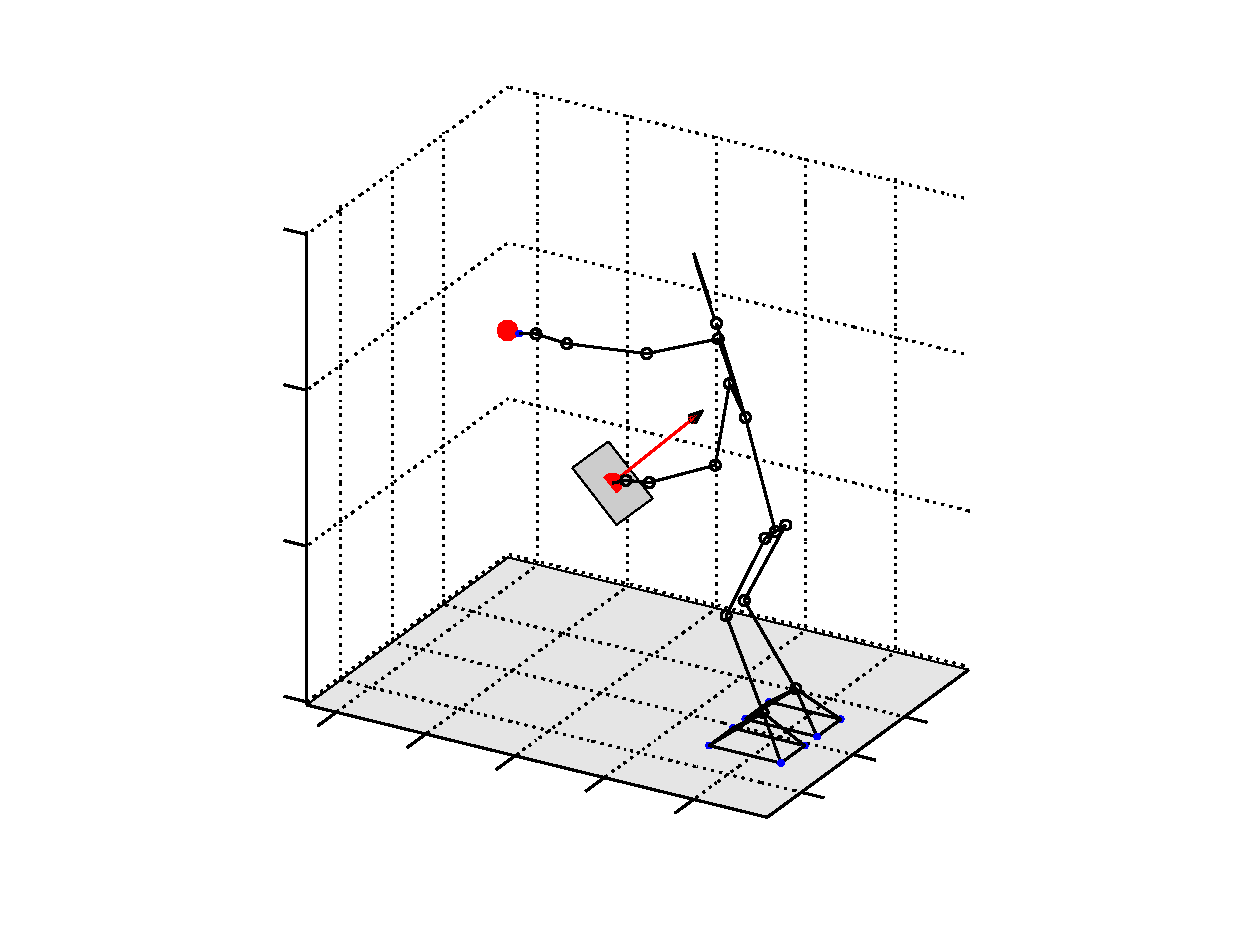
\includegraphics[trim=50  46  50   0,clip,scale=0.42]{test_17_23_robot_2001-inc}
\end{picture}%
\begin{picture}(476, 386)(50,46)
\fontsize{7}{0}
\selectfont\put(123.469,106.786){\makebox(0,0)[br]{\textcolor[rgb]{0,0,0}{{0}}}}
\fontsize{7}{0}
\selectfont\put(123.469,181.561){\makebox(0,0)[br]{\textcolor[rgb]{0,0,0}{{0.5}}}}
\fontsize{7}{0}
\selectfont\put(123.469,256.337){\makebox(0,0)[br]{\textcolor[rgb]{0,0,0}{{1}}}}
\fontsize{7}{0}
\selectfont\put(123.469,331.112){\makebox(0,0)[br]{\textcolor[rgb]{0,0,0}{{1.5}}}}
\fontsize{7}{0}
\selectfont\put(140.455,88.4511){\makebox(0,0)[tr]{\textcolor[rgb]{0,0,0}{{1.2}}}}
\fontsize{7}{0}
\selectfont\put(183.326,77.9906){\makebox(0,0)[tr]{\textcolor[rgb]{0,0,0}{{0.9}}}}
\fontsize{7}{0}
\selectfont\put(226.197,67.5301){\makebox(0,0)[tr]{\textcolor[rgb]{0,0,0}{{0.6}}}}
\fontsize{7}{0}
\selectfont\put(269.068,57.0696){\makebox(0,0)[tr]{\textcolor[rgb]{0,0,0}{{0.3}}}}
\fontsize{7}{0}
\selectfont\put(311.939,46.6091){\makebox(0,0)[tr]{\textcolor[rgb]{0,0,0}{{0}}}}
\fontsize{7}{0}
\selectfont\put(441.858,91.9431){\makebox(0,0)[tl]{\textcolor[rgb]{0,0,0}{{-0.3}}}}
\fontsize{7}{0}
\selectfont\put(417.107,73.825){\makebox(0,0)[tl]{\textcolor[rgb]{0,0,0}{{0}}}}
\fontsize{7}{0}
\selectfont\put(392.355,55.7069){\makebox(0,0)[tl]{\textcolor[rgb]{0,0,0}{{0.3}}}}
\end{picture}

            \subcaption{after $10$ seconds}
            \label{fig.force_distrib.3}
        }
    \end{minipage}
    \hfill
    \begin{minipage}[t]{0.49\textwidth}
        \centering{
            % Title: glps_renderer figure
% Creator: GL2PS 1.3.8, (C) 1999-2012 C. Geuzaine
% For: Octave
% CreationDate: Mon May  9 19:27:12 2016
\setlength{\unitlength}{0.42pt}
\begin{picture}(0,0)
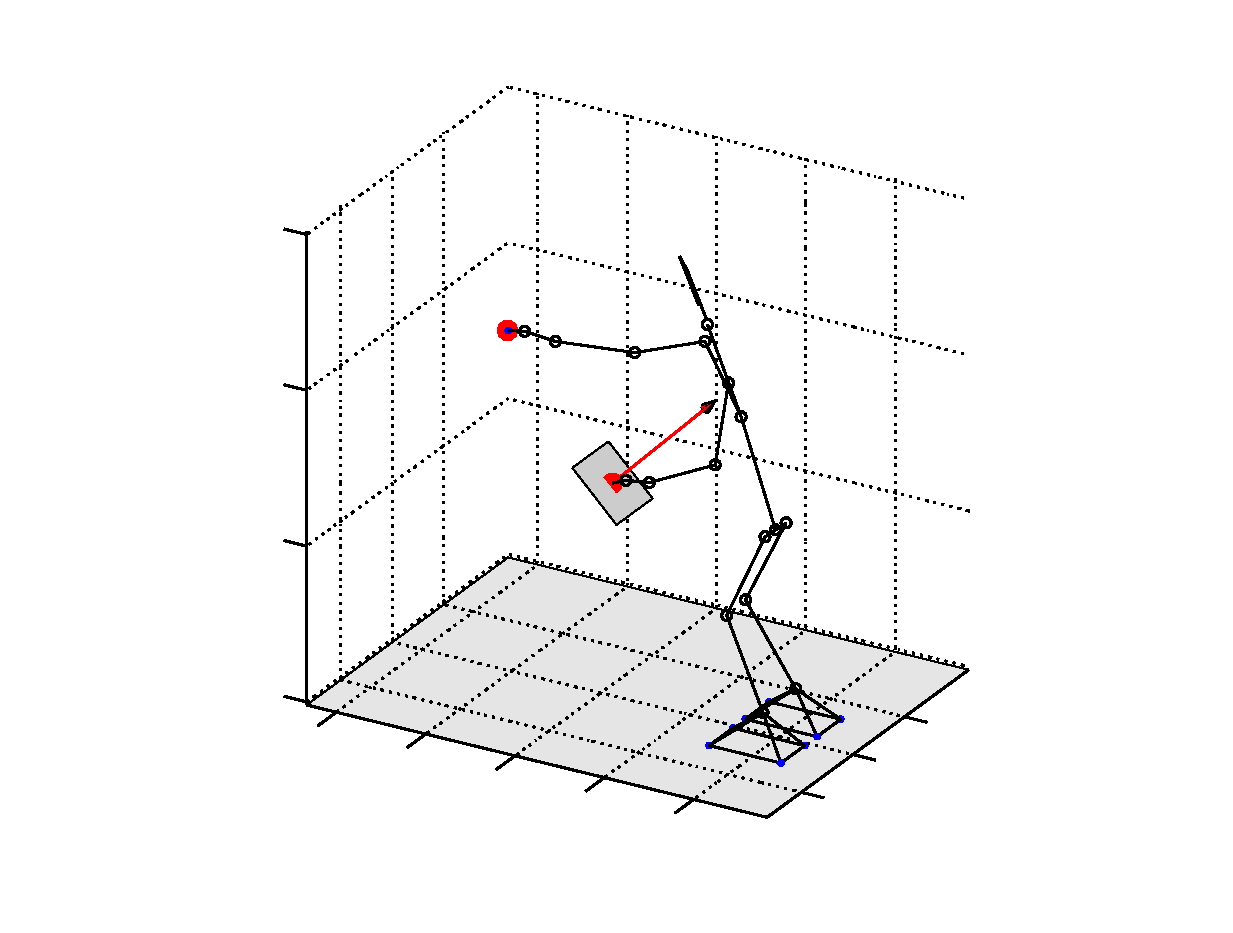
\includegraphics[trim=50  46  50   0,clip,scale=0.42]{test_17_23_robot_3001-inc}
\end{picture}%
\begin{picture}(476, 386)(50,46)
\fontsize{7}{0}
\selectfont\put(123.469,106.786){\makebox(0,0)[br]{\textcolor[rgb]{0,0,0}{{0}}}}
\fontsize{7}{0}
\selectfont\put(123.469,181.561){\makebox(0,0)[br]{\textcolor[rgb]{0,0,0}{{0.5}}}}
\fontsize{7}{0}
\selectfont\put(123.469,256.337){\makebox(0,0)[br]{\textcolor[rgb]{0,0,0}{{1}}}}
\fontsize{7}{0}
\selectfont\put(123.469,331.112){\makebox(0,0)[br]{\textcolor[rgb]{0,0,0}{{1.5}}}}
\fontsize{7}{0}
\selectfont\put(140.455,88.4511){\makebox(0,0)[tr]{\textcolor[rgb]{0,0,0}{{1.2}}}}
\fontsize{7}{0}
\selectfont\put(183.326,77.9906){\makebox(0,0)[tr]{\textcolor[rgb]{0,0,0}{{0.9}}}}
\fontsize{7}{0}
\selectfont\put(226.197,67.5301){\makebox(0,0)[tr]{\textcolor[rgb]{0,0,0}{{0.6}}}}
\fontsize{7}{0}
\selectfont\put(269.068,57.0696){\makebox(0,0)[tr]{\textcolor[rgb]{0,0,0}{{0.3}}}}
\fontsize{7}{0}
\selectfont\put(311.939,46.6091){\makebox(0,0)[tr]{\textcolor[rgb]{0,0,0}{{0}}}}
\fontsize{7}{0}
\selectfont\put(441.858,91.9431){\makebox(0,0)[tl]{\textcolor[rgb]{0,0,0}{{-0.3}}}}
\fontsize{7}{0}
\selectfont\put(417.107,73.825){\makebox(0,0)[tl]{\textcolor[rgb]{0,0,0}{{0}}}}
\fontsize{7}{0}
\selectfont\put(392.355,55.7069){\makebox(0,0)[tl]{\textcolor[rgb]{0,0,0}{{0.3}}}}
\end{picture}

            \subcaption{after $15$ seconds}
            \label{fig.force_distrib.4}
        }
    \end{minipage}
    \begin{minipage}[t]{0.49\textwidth}
        \centering{
            % Title: glps_renderer figure
% Creator: GL2PS 1.3.8, (C) 1999-2012 C. Geuzaine
% For: Octave
% CreationDate: Mon May  9 19:27:13 2016
\setlength{\unitlength}{0.42pt}
\begin{picture}(0,0)
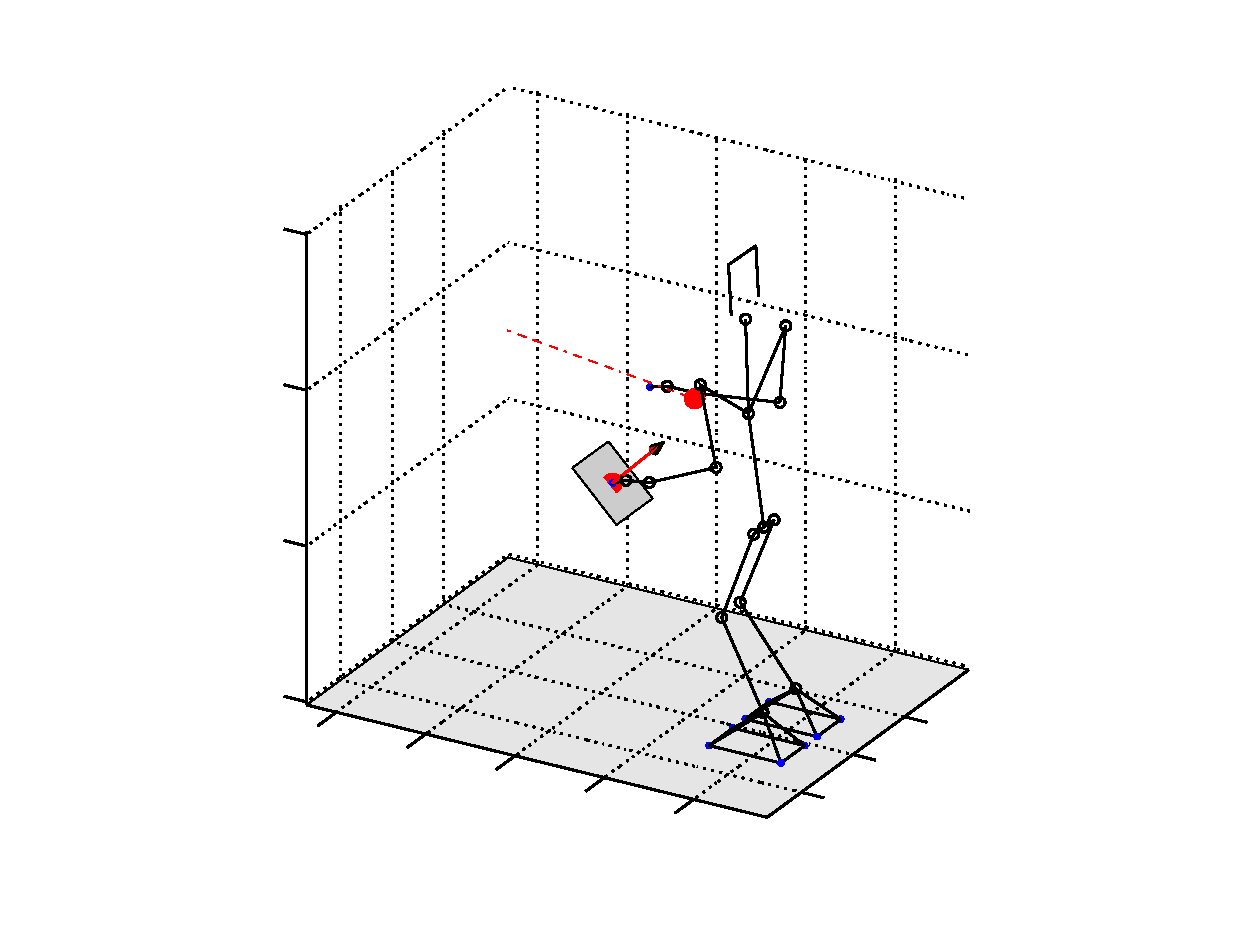
\includegraphics[trim=50  46  50   0,clip,scale=0.42]{test_17_23_robot_4001-inc}
\end{picture}%
\begin{picture}(476, 386)(50,46)
\fontsize{7}{0}
\selectfont\put(123.469,106.786){\makebox(0,0)[br]{\textcolor[rgb]{0,0,0}{{0}}}}
\fontsize{7}{0}
\selectfont\put(123.469,181.561){\makebox(0,0)[br]{\textcolor[rgb]{0,0,0}{{0.5}}}}
\fontsize{7}{0}
\selectfont\put(123.469,256.337){\makebox(0,0)[br]{\textcolor[rgb]{0,0,0}{{1}}}}
\fontsize{7}{0}
\selectfont\put(123.469,331.112){\makebox(0,0)[br]{\textcolor[rgb]{0,0,0}{{1.5}}}}
\fontsize{7}{0}
\selectfont\put(140.455,88.4511){\makebox(0,0)[tr]{\textcolor[rgb]{0,0,0}{{1.2}}}}
\fontsize{7}{0}
\selectfont\put(183.326,77.9906){\makebox(0,0)[tr]{\textcolor[rgb]{0,0,0}{{0.9}}}}
\fontsize{7}{0}
\selectfont\put(226.197,67.5301){\makebox(0,0)[tr]{\textcolor[rgb]{0,0,0}{{0.6}}}}
\fontsize{7}{0}
\selectfont\put(269.068,57.0696){\makebox(0,0)[tr]{\textcolor[rgb]{0,0,0}{{0.3}}}}
\fontsize{7}{0}
\selectfont\put(311.939,46.6091){\makebox(0,0)[tr]{\textcolor[rgb]{0,0,0}{{0}}}}
\fontsize{7}{0}
\selectfont\put(441.858,91.9431){\makebox(0,0)[tl]{\textcolor[rgb]{0,0,0}{{-0.3}}}}
\fontsize{7}{0}
\selectfont\put(417.107,73.825){\makebox(0,0)[tl]{\textcolor[rgb]{0,0,0}{{0}}}}
\fontsize{7}{0}
\selectfont\put(392.355,55.7069){\makebox(0,0)[tl]{\textcolor[rgb]{0,0,0}{{0.3}}}}
\end{picture}

            \subcaption{after $20$ seconds}
            \label{fig.force_distrib.5}
        }
    \end{minipage}
    \hfill
    \begin{minipage}[t]{0.49\textwidth}
        \centering{
            % Title: glps_renderer figure
% Creator: GL2PS 1.3.8, (C) 1999-2012 C. Geuzaine
% For: Octave
% CreationDate: Mon May  9 19:27:15 2016
\setlength{\unitlength}{0.42pt}
\begin{picture}(0,0)
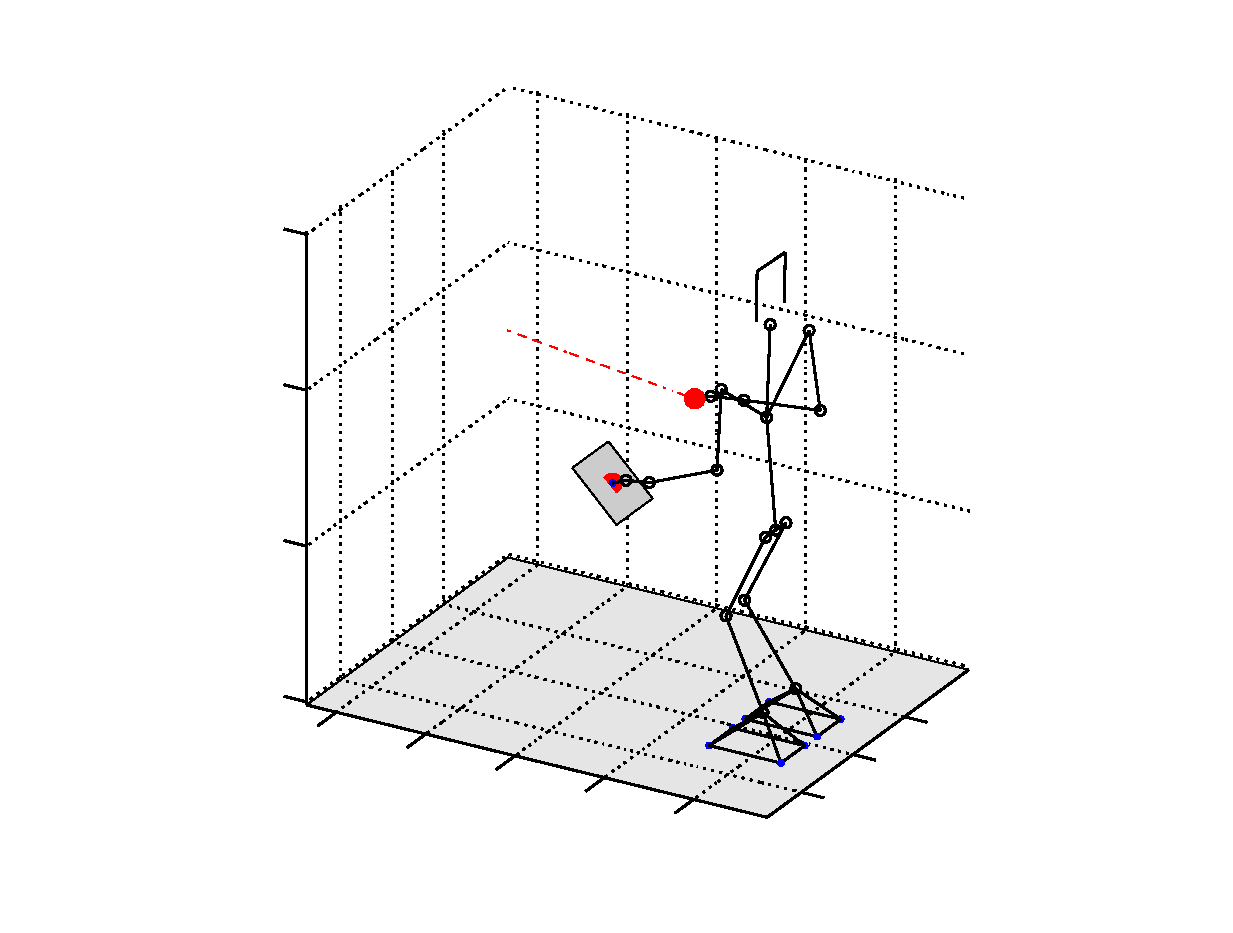
\includegraphics[trim=50  46  50   0,clip,scale=0.42]{test_17_23_robot_5000-inc}
\end{picture}%
\begin{picture}(476, 386)(50,46)
\fontsize{7}{0}
\selectfont\put(123.469,106.786){\makebox(0,0)[br]{\textcolor[rgb]{0,0,0}{{0}}}}
\fontsize{7}{0}
\selectfont\put(123.469,181.561){\makebox(0,0)[br]{\textcolor[rgb]{0,0,0}{{0.5}}}}
\fontsize{7}{0}
\selectfont\put(123.469,256.337){\makebox(0,0)[br]{\textcolor[rgb]{0,0,0}{{1}}}}
\fontsize{7}{0}
\selectfont\put(123.469,331.112){\makebox(0,0)[br]{\textcolor[rgb]{0,0,0}{{1.5}}}}
\fontsize{7}{0}
\selectfont\put(441.858,91.9431){\makebox(0,0)[tl]{\textcolor[rgb]{0,0,0}{{-0.3}}}}
\fontsize{7}{0}
\selectfont\put(140.455,88.4511){\makebox(0,0)[tr]{\textcolor[rgb]{0,0,0}{{1.2}}}}
\fontsize{7}{0}
\selectfont\put(183.326,77.9906){\makebox(0,0)[tr]{\textcolor[rgb]{0,0,0}{{0.9}}}}
\fontsize{7}{0}
\selectfont\put(417.107,73.825){\makebox(0,0)[tl]{\textcolor[rgb]{0,0,0}{{0}}}}
\fontsize{7}{0}
\selectfont\put(226.197,67.5301){\makebox(0,0)[tr]{\textcolor[rgb]{0,0,0}{{0.6}}}}
\fontsize{7}{0}
\selectfont\put(269.068,57.0696){\makebox(0,0)[tr]{\textcolor[rgb]{0,0,0}{{0.3}}}}
\fontsize{7}{0}
\selectfont\put(311.939,46.6091){\makebox(0,0)[tr]{\textcolor[rgb]{0,0,0}{{0}}}}
\fontsize{7}{0}
\selectfont\put(392.355,55.7069){\makebox(0,0)[tl]{\textcolor[rgb]{0,0,0}{{0.3}}}}
\end{picture}

            \subcaption{after $30$ seconds}
            \label{fig.force_distrib.6}
        }
    \end{minipage}
    \caption[Prioritization of the contact forces: reaching task.]{
        Configurations of the robot while it is trying to reach a target
        indicated by the red point. Grey areas represent contact surfaces.
        Length of the arrow indicates magnitude of the contact force applied by
        the left hand.
    }
    \label{fig.force_distrib}
\end{figure}


We use the following setting: the robot is standing with its left hand
positioned on an additional support, while the right hand executes certain
task. Hence, the number of contacts $M = 3$ (two feet and the hand) is constant
during the simulations. We define two different hand tasks. In the first case
the robot has to reach a target, which is initially unreachable without using
the additional support and later moved closer to the robot (see
\cref{fig.force_distrib,fig.force_distrib_right_hand}). The second task is to
maintain position of the right hand while an external disturbing force is
acting on it (see \cref{fig.force_distrib_weight}). In other words, the robot
holds a heavy object, such as a filled bucket \cite{Stephens2010iros}. The
external force is varying with time and is assumed to be measured. In all tests
the controller is expected to apply a force on the additional support only if
necessary to preserve balance and execute the hand task.


\begin{figure}[!htbp]
    \centering{
        % Title: glps_renderer figure
% Creator: GL2PS 1.3.8, (C) 1999-2012 C. Geuzaine
% For: Octave
% CreationDate: Mon May  9 19:44:30 2016
\setlength{\unitlength}{0.5pt}
\begin{picture}(0,0)
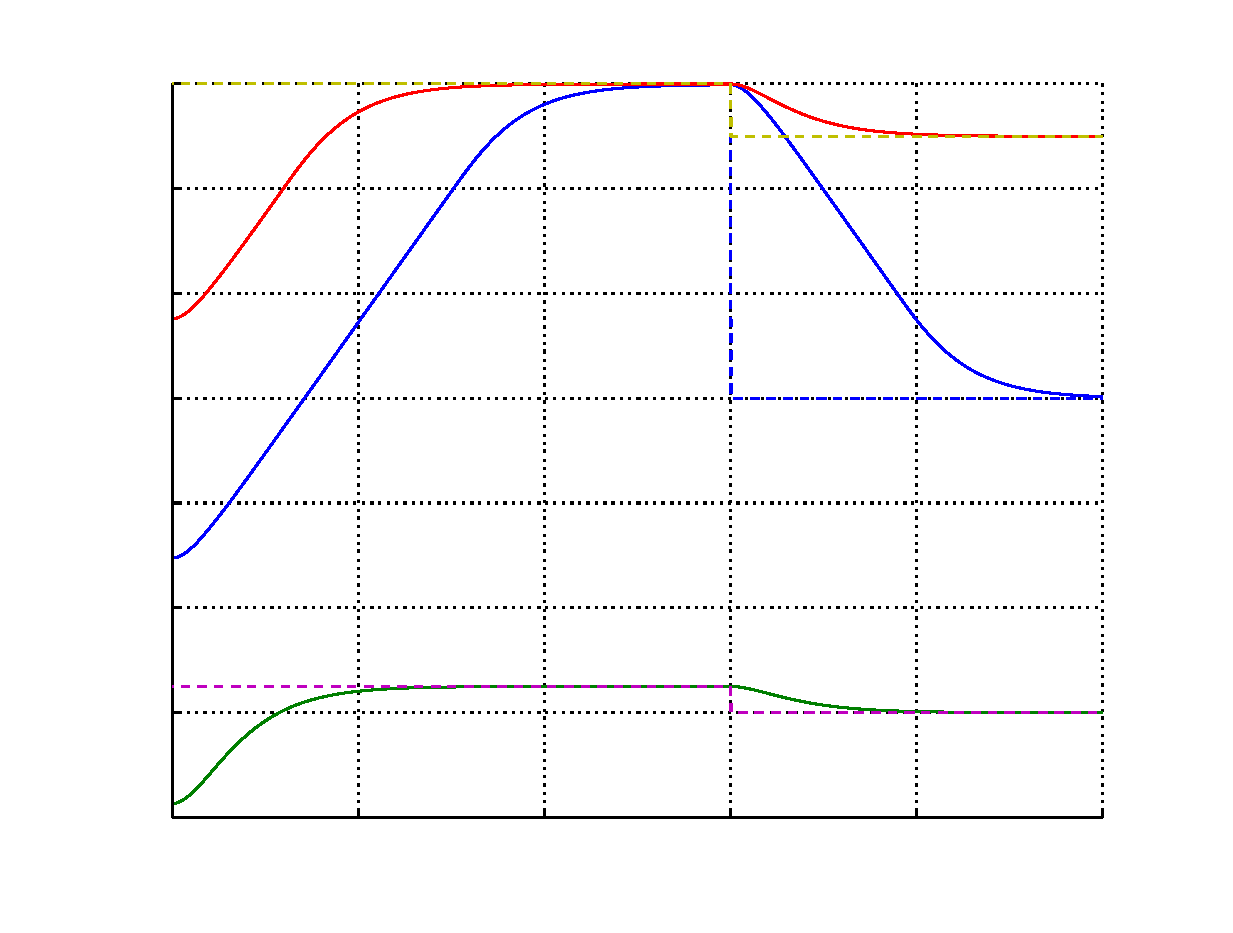
\includegraphics[trim=0  0  0  0,clip,scale=0.5]{test_17_23_position-inc}
\end{picture}%
\begin{picture}(576, 432)(0,0)
\fontsize{11}{0}
\selectfont\put(74.88,42.5189){\makebox(0,0)[t]{\textcolor[rgb]{0,0,0}{{0}}}}
\fontsize{11}{0}
\selectfont\put(164.16,42.5189){\makebox(0,0)[t]{\textcolor[rgb]{0,0,0}{{5}}}}
\fontsize{11}{0}
\selectfont\put(253.44,42.5189){\makebox(0,0)[t]{\textcolor[rgb]{0,0,0}{{10}}}}
\fontsize{11}{0}
\selectfont\put(342.72,42.5189){\makebox(0,0)[t]{\textcolor[rgb]{0,0,0}{{15}}}}
\fontsize{11}{0}
\selectfont\put(432,42.5189){\makebox(0,0)[t]{\textcolor[rgb]{0,0,0}{{20}}}}
\fontsize{11}{0}
\selectfont\put(521.28,42.5189){\makebox(0,0)[t]{\textcolor[rgb]{0,0,0}{{25}}}}
\fontsize{11}{0}
\selectfont\put(69.8755,47.52){\makebox(0,0)[r]{\textcolor[rgb]{0,0,0}{{-0.4}}}}
\fontsize{11}{0}
\selectfont\put(69.8755,97.8171){\makebox(0,0)[r]{\textcolor[rgb]{0,0,0}{{-0.2}}}}
\fontsize{11}{0}
\selectfont\put(69.8755,148.114){\makebox(0,0)[r]{\textcolor[rgb]{0,0,0}{{0}}}}
\fontsize{11}{0}
\selectfont\put(69.8755,198.411){\makebox(0,0)[r]{\textcolor[rgb]{0,0,0}{{0.2}}}}
\fontsize{11}{0}
\selectfont\put(69.8755,248.709){\makebox(0,0)[r]{\textcolor[rgb]{0,0,0}{{0.4}}}}
\fontsize{11}{0}
\selectfont\put(69.8755,299.006){\makebox(0,0)[r]{\textcolor[rgb]{0,0,0}{{0.6}}}}
\fontsize{11}{0}
\selectfont\put(69.8755,349.303){\makebox(0,0)[r]{\textcolor[rgb]{0,0,0}{{0.8}}}}
\fontsize{11}{0}
\selectfont\put(69.8755,399.6){\makebox(0,0)[r]{\textcolor[rgb]{0,0,0}{{1}}}}
\fontsize{11}{0}
\selectfont\put(298.08,26.5189){\makebox(0,0)[t]{\textcolor[rgb]{0,0,0}{{simulation time $[s]$}}}}
\fontsize{11}{0}
\selectfont\put(40.8755,223.56){\rotatebox{90}{\makebox(0,0)[b]{\textcolor[rgb]{0,0,0}{{right hand position $[m]$}}}}}
\end{picture}

        \caption[Execution of the reaching right hand task.]{
            Position of the right hand during execution of the reaching task.
            $x$, $y$, and $z$ coordinates are shown in solid blue, green, and
            red respectively. The desired positions are shown in dashed lines.
        }
        \label{fig.force_distrib_right_hand}
    }
\end{figure}


\begin{figure}[!htbp]
    \begin{minipage}[t]{0.49\textwidth}
        \centering{
            % Title: glps_renderer figure
% Creator: GL2PS 1.3.8, (C) 1999-2012 C. Geuzaine
% For: Octave
% CreationDate: Fri Mar 18 18:16:03 2016
\setlength{\unitlength}{0.42pt}
\begin{picture}(0,0)
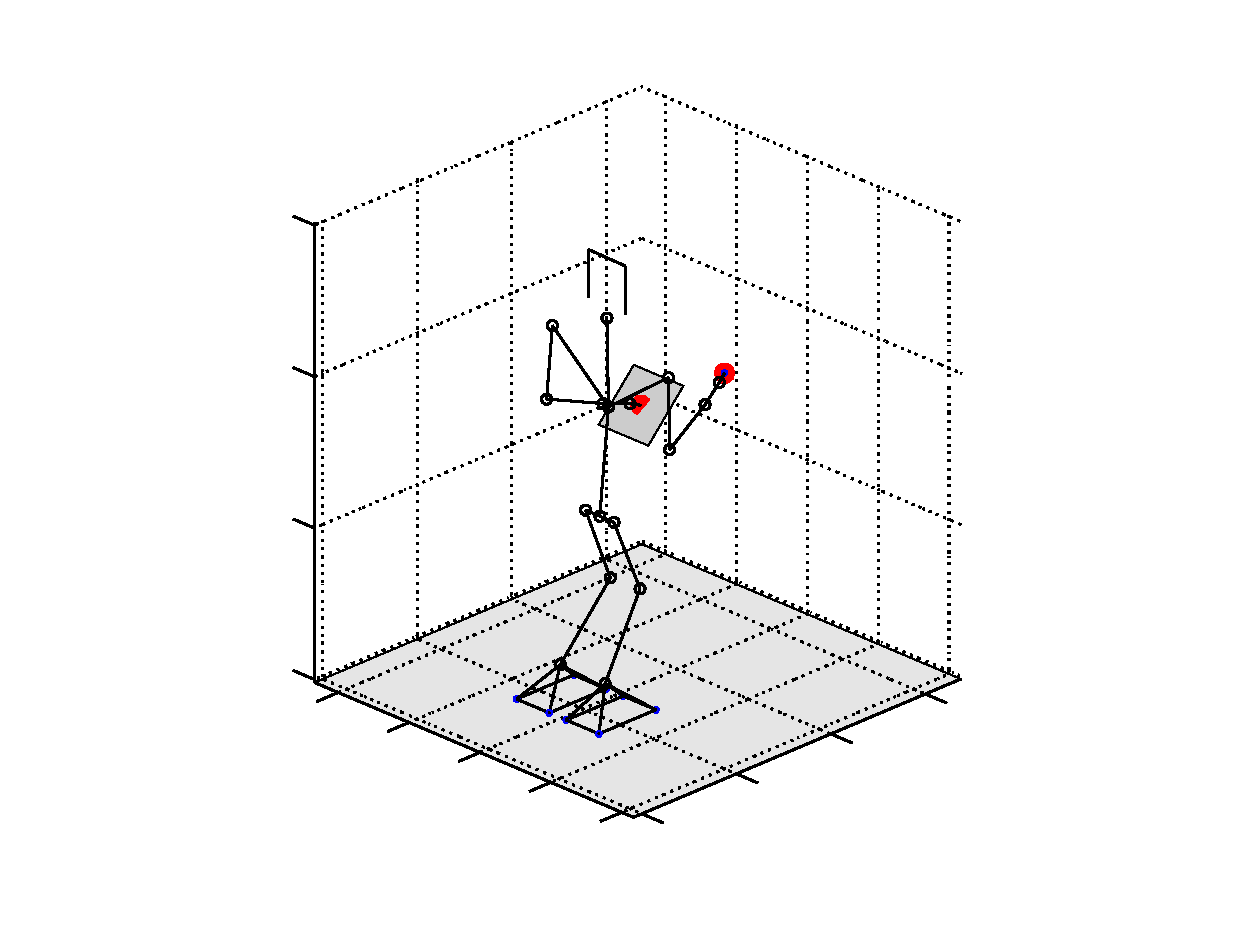
\includegraphics[trim=50  40  50  15,clip,scale=0.42]{test_17_24_robot_1-inc}
\end{picture}%
\begin{picture}(476, 377)(50,40)
\fontsize{8}{0}
\selectfont\put(128.078,119.977){\makebox(0,0)[br]{\textcolor[rgb]{0,0,0}{{0}}}}
\fontsize{8}{0}
\selectfont\put(128.078,192.665){\makebox(0,0)[br]{\textcolor[rgb]{0,0,0}{{0.5}}}}
\fontsize{8}{0}
\selectfont\put(128.078,265.352){\makebox(0,0)[br]{\textcolor[rgb]{0,0,0}{{1}}}}
\fontsize{8}{0}
\selectfont\put(128.078,338.039){\makebox(0,0)[br]{\textcolor[rgb]{0,0,0}{{1.5}}}}
\fontsize{8}{0}
\selectfont\put(451.064,100.435){\makebox(0,0)[tl]{\textcolor[rgb]{0,0,0}{{0.8}}}}
\fontsize{8}{0}
\selectfont\put(139.398,101.139){\makebox(0,0)[tr]{\textcolor[rgb]{0,0,0}{{0.6}}}}
\fontsize{8}{0}
\selectfont\put(173.424,86.7588){\makebox(0,0)[tr]{\textcolor[rgb]{0,0,0}{{0.3}}}}
\fontsize{8}{0}
\selectfont\put(207.451,72.3785){\makebox(0,0)[tr]{\textcolor[rgb]{0,0,0}{{0}}}}
\fontsize{8}{0}
\selectfont\put(241.478,57.9982){\makebox(0,0)[tr]{\textcolor[rgb]{0,0,0}{{-0.3}}}}
\fontsize{8}{0}
\selectfont\put(275.504,43.6179){\makebox(0,0)[tr]{\textcolor[rgb]{0,0,0}{{-0.6}}}}
\fontsize{8}{0}
\selectfont\put(314.957,42.9134){\makebox(0,0)[tl]{\textcolor[rgb]{0,0,0}{{-0.4}}}}
\fontsize{8}{0}
\selectfont\put(360.326,62.0872){\makebox(0,0)[tl]{\textcolor[rgb]{0,0,0}{{0}}}}
\fontsize{8}{0}
\selectfont\put(405.695,81.2609){\makebox(0,0)[tl]{\textcolor[rgb]{0,0,0}{{0.4}}}}
\end{picture}

            \subcaption{initial configuration}
            \label{fig.force_distrib_weight.1}
        }
    \end{minipage}
    \hfill
    \begin{minipage}[t]{0.49\textwidth}
        \centering{
            % Title: glps_renderer figure
% Creator: GL2PS 1.3.8, (C) 1999-2012 C. Geuzaine
% For: Octave
% CreationDate: Fri Mar 18 18:16:05 2016
\setlength{\unitlength}{0.42pt}
\begin{picture}(0,0)
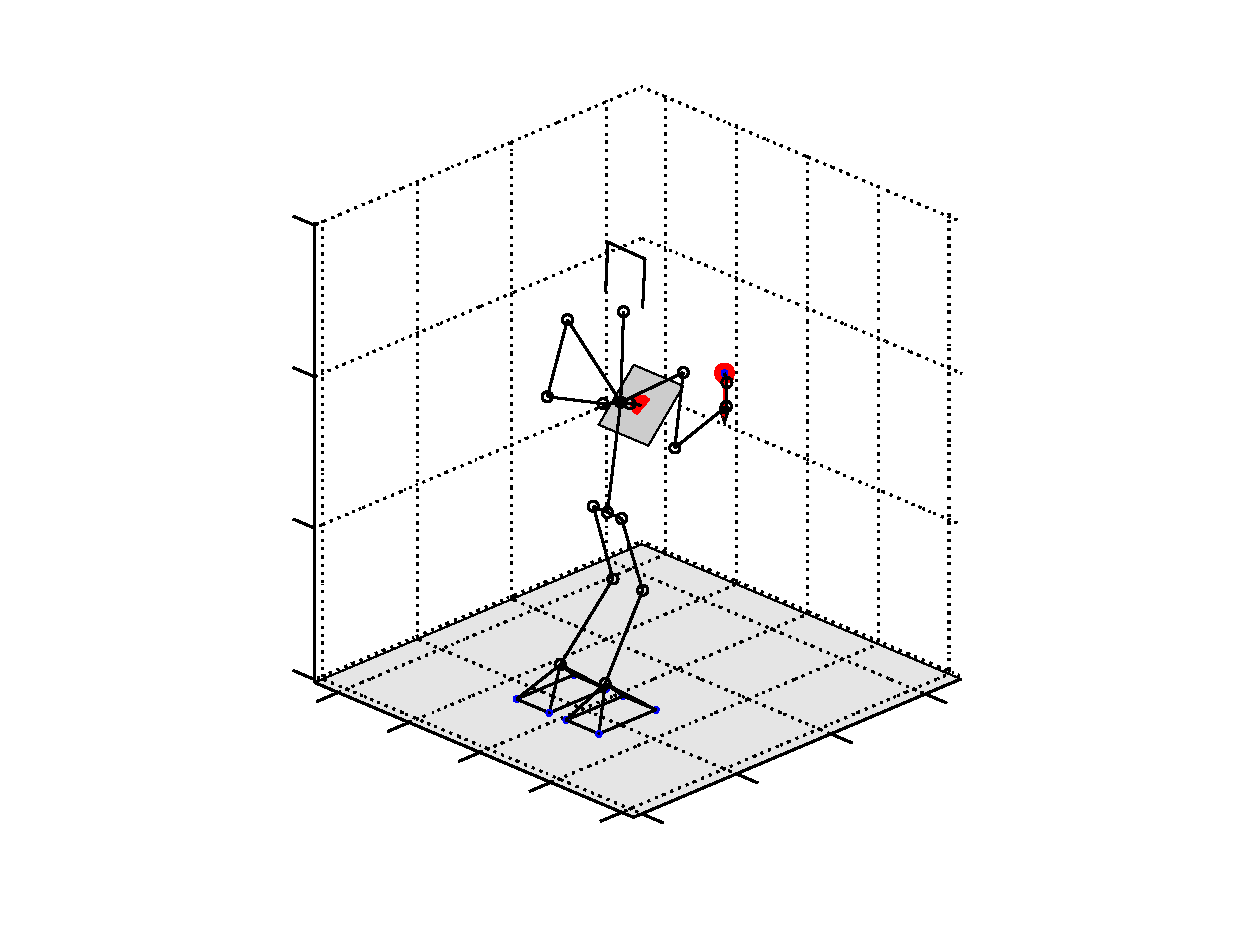
\includegraphics[trim=50  40  50  15,clip,scale=0.42]{test_17_24_robot_401-inc}
\end{picture}%
\begin{picture}(476, 377)(50,40)
\fontsize{8}{0}
\selectfont\put(128.078,119.977){\makebox(0,0)[br]{\textcolor[rgb]{0,0,0}{{0}}}}
\fontsize{8}{0}
\selectfont\put(128.078,192.665){\makebox(0,0)[br]{\textcolor[rgb]{0,0,0}{{0.5}}}}
\fontsize{8}{0}
\selectfont\put(128.078,265.352){\makebox(0,0)[br]{\textcolor[rgb]{0,0,0}{{1}}}}
\fontsize{8}{0}
\selectfont\put(128.078,338.039){\makebox(0,0)[br]{\textcolor[rgb]{0,0,0}{{1.5}}}}
\fontsize{8}{0}
\selectfont\put(451.064,100.435){\makebox(0,0)[tl]{\textcolor[rgb]{0,0,0}{{0.8}}}}
\fontsize{8}{0}
\selectfont\put(360.326,62.0872){\makebox(0,0)[tl]{\textcolor[rgb]{0,0,0}{{0}}}}
\fontsize{8}{0}
\selectfont\put(405.695,81.2609){\makebox(0,0)[tl]{\textcolor[rgb]{0,0,0}{{0.4}}}}
\fontsize{8}{0}
\selectfont\put(173.424,86.7588){\makebox(0,0)[tr]{\textcolor[rgb]{0,0,0}{{0.3}}}}
\fontsize{8}{0}
\selectfont\put(139.398,101.139){\makebox(0,0)[tr]{\textcolor[rgb]{0,0,0}{{0.6}}}}
\fontsize{8}{0}
\selectfont\put(207.451,72.3785){\makebox(0,0)[tr]{\textcolor[rgb]{0,0,0}{{0}}}}
\fontsize{8}{0}
\selectfont\put(241.478,57.9982){\makebox(0,0)[tr]{\textcolor[rgb]{0,0,0}{{-0.3}}}}
\fontsize{8}{0}
\selectfont\put(275.504,43.6179){\makebox(0,0)[tr]{\textcolor[rgb]{0,0,0}{{-0.6}}}}
\fontsize{8}{0}
\selectfont\put(314.957,42.9134){\makebox(0,0)[tl]{\textcolor[rgb]{0,0,0}{{-0.4}}}}
\fontsize{8}{0}
\selectfont\put(339.763,236.509){\makebox(0,0)[l]{\textcolor[rgb]{0,0,0}{{$\V{f}_{\MT{rh}}$}}}}
\end{picture}

            \subcaption{after $2$ seconds}
            \label{fig.force_distrib_weight.2}
        }
    \end{minipage}
    \begin{minipage}[t]{0.49\textwidth}
        \centering{
            % Title: glps_renderer figure
% Creator: GL2PS 1.3.8, (C) 1999-2012 C. Geuzaine
% For: Octave
% CreationDate: Fri Mar 18 18:16:06 2016
\setlength{\unitlength}{0.42pt}
\begin{picture}(0,0)
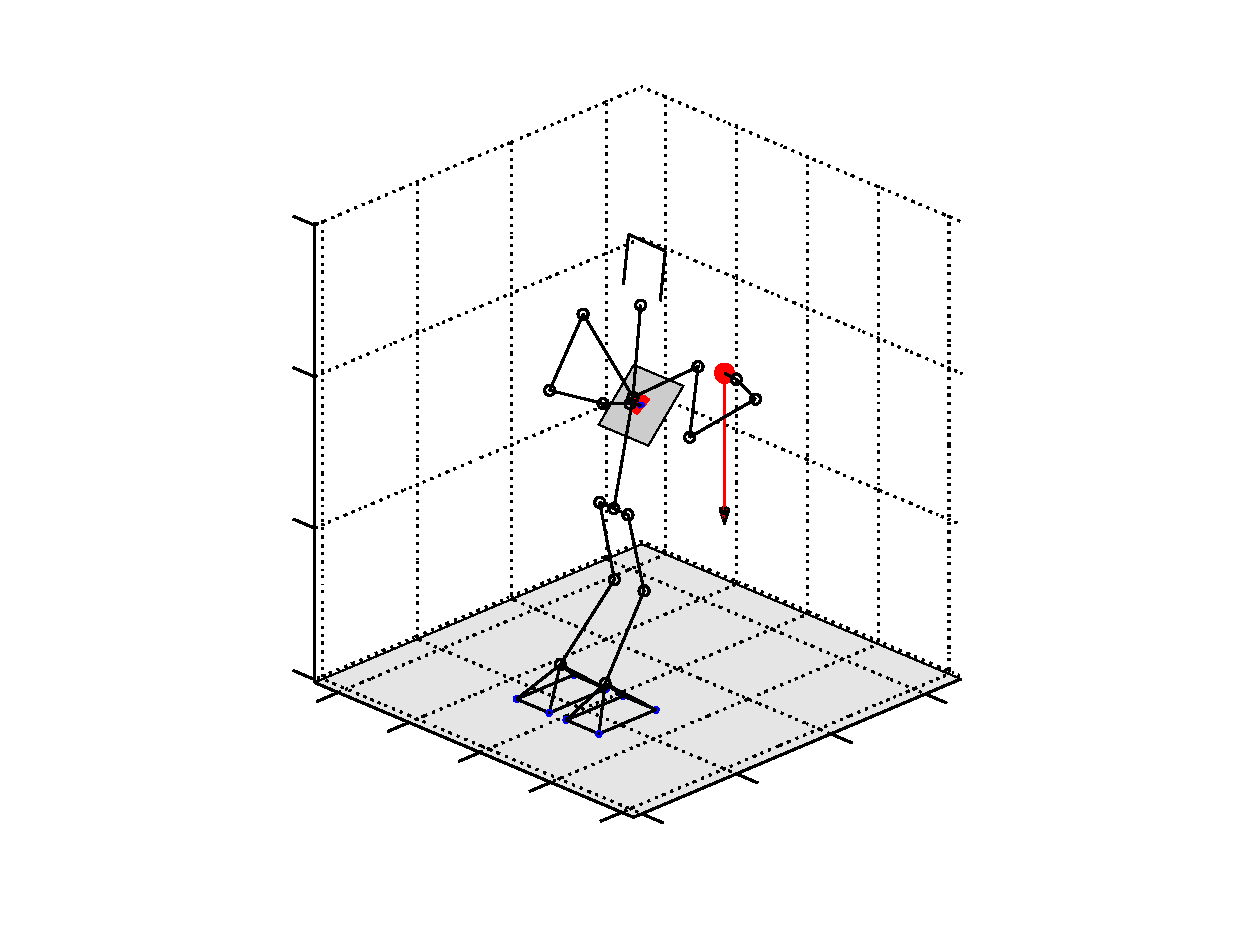
\includegraphics[trim=50  40  50  15,clip,scale=0.42]{test_17_24_robot_1001-inc}
\end{picture}%
\begin{picture}(476, 377)(50,40)
\fontsize{8}{0}
\selectfont\put(128.078,119.977){\makebox(0,0)[br]{\textcolor[rgb]{0,0,0}{{0}}}}
\fontsize{8}{0}
\selectfont\put(128.078,192.665){\makebox(0,0)[br]{\textcolor[rgb]{0,0,0}{{0.5}}}}
\fontsize{8}{0}
\selectfont\put(128.078,265.352){\makebox(0,0)[br]{\textcolor[rgb]{0,0,0}{{1}}}}
\fontsize{8}{0}
\selectfont\put(128.078,338.039){\makebox(0,0)[br]{\textcolor[rgb]{0,0,0}{{1.5}}}}
\fontsize{8}{0}
\selectfont\put(360.326,62.0872){\makebox(0,0)[tl]{\textcolor[rgb]{0,0,0}{{0}}}}
\fontsize{8}{0}
\selectfont\put(405.695,81.2609){\makebox(0,0)[tl]{\textcolor[rgb]{0,0,0}{{0.4}}}}
\fontsize{8}{0}
\selectfont\put(451.064,100.435){\makebox(0,0)[tl]{\textcolor[rgb]{0,0,0}{{0.8}}}}
\fontsize{8}{0}
\selectfont\put(339.766,188.063){\makebox(0,0)[l]{\textcolor[rgb]{0,0,0}{{$\V{f}_{\MT{rh}}$}}}}
\fontsize{8}{0}
\selectfont\put(173.424,86.7588){\makebox(0,0)[tr]{\textcolor[rgb]{0,0,0}{{0.3}}}}
\fontsize{8}{0}
\selectfont\put(139.398,101.139){\makebox(0,0)[tr]{\textcolor[rgb]{0,0,0}{{0.6}}}}
\fontsize{8}{0}
\selectfont\put(207.451,72.3785){\makebox(0,0)[tr]{\textcolor[rgb]{0,0,0}{{0}}}}
\fontsize{8}{0}
\selectfont\put(241.478,57.9982){\makebox(0,0)[tr]{\textcolor[rgb]{0,0,0}{{-0.3}}}}
\fontsize{8}{0}
\selectfont\put(275.504,43.6179){\makebox(0,0)[tr]{\textcolor[rgb]{0,0,0}{{-0.6}}}}
\fontsize{8}{0}
\selectfont\put(314.957,42.9134){\makebox(0,0)[tl]{\textcolor[rgb]{0,0,0}{{-0.4}}}}
\end{picture}

            \subcaption{after $5$ seconds}
            \label{fig.force_distrib_weight.3}
        }
    \end{minipage}
    \hfill
    \begin{minipage}[t]{0.49\textwidth}
        \centering{
            % Title: glps_renderer figure
% Creator: GL2PS 1.3.8, (C) 1999-2012 C. Geuzaine
% For: Octave
% CreationDate: Fri Mar 18 18:16:07 2016
\setlength{\unitlength}{0.42pt}
\begin{picture}(0,0)
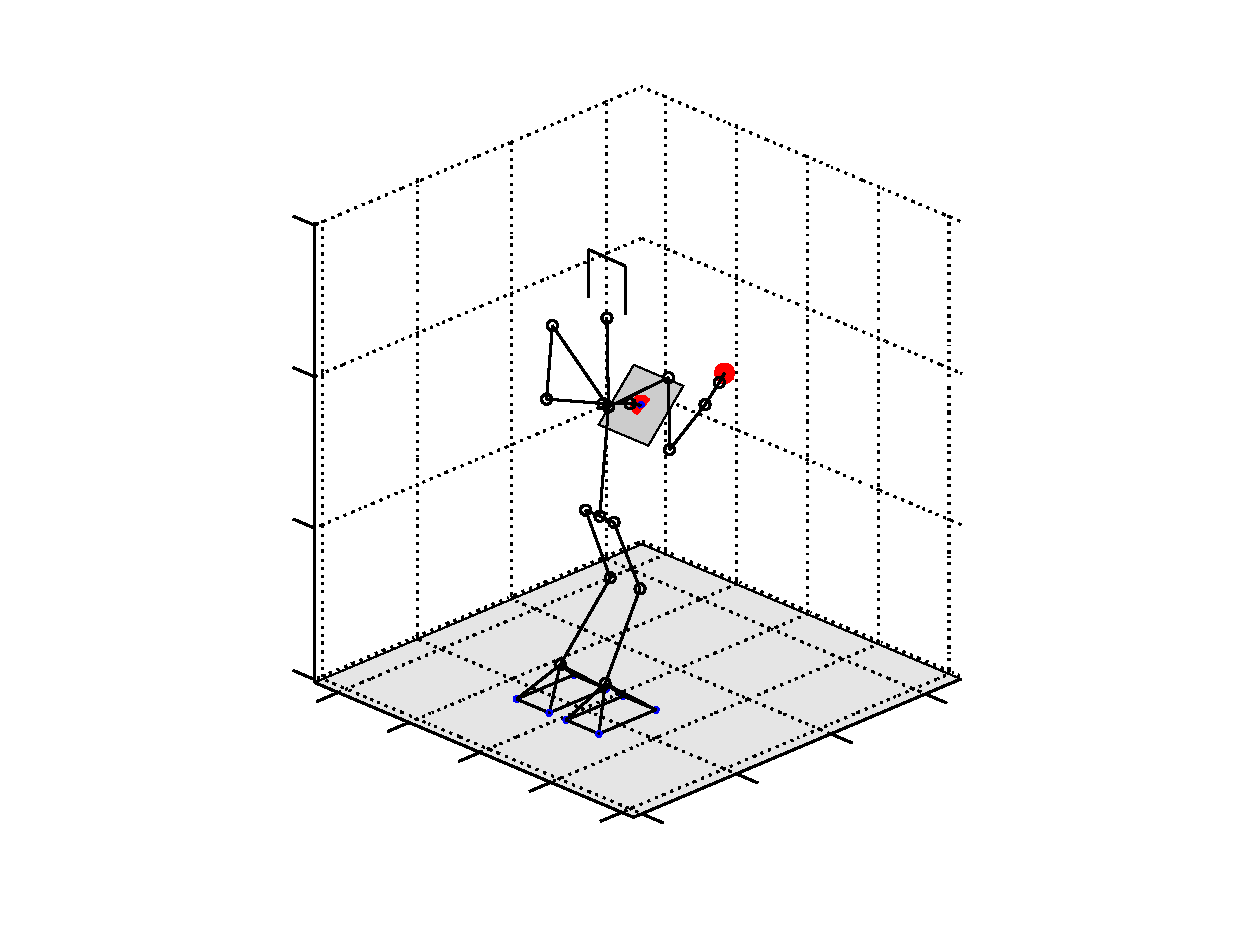
\includegraphics[trim=50  40  50  15,clip,scale=0.42]{test_17_24_robot_2000-inc}
\end{picture}%
\begin{picture}(476, 377)(50,40)
\fontsize{8}{0}
\selectfont\put(128.078,119.977){\makebox(0,0)[br]{\textcolor[rgb]{0,0,0}{{0}}}}
\fontsize{8}{0}
\selectfont\put(128.078,192.665){\makebox(0,0)[br]{\textcolor[rgb]{0,0,0}{{0.5}}}}
\fontsize{8}{0}
\selectfont\put(128.078,265.352){\makebox(0,0)[br]{\textcolor[rgb]{0,0,0}{{1}}}}
\fontsize{8}{0}
\selectfont\put(128.078,338.039){\makebox(0,0)[br]{\textcolor[rgb]{0,0,0}{{1.5}}}}
\fontsize{8}{0}
\selectfont\put(451.064,100.435){\makebox(0,0)[tl]{\textcolor[rgb]{0,0,0}{{0.8}}}}
\fontsize{8}{0}
\selectfont\put(139.398,101.139){\makebox(0,0)[tr]{\textcolor[rgb]{0,0,0}{{0.6}}}}
\fontsize{8}{0}
\selectfont\put(173.424,86.7588){\makebox(0,0)[tr]{\textcolor[rgb]{0,0,0}{{0.3}}}}
\fontsize{8}{0}
\selectfont\put(207.451,72.3785){\makebox(0,0)[tr]{\textcolor[rgb]{0,0,0}{{0}}}}
\fontsize{8}{0}
\selectfont\put(241.478,57.9982){\makebox(0,0)[tr]{\textcolor[rgb]{0,0,0}{{-0.3}}}}
\fontsize{8}{0}
\selectfont\put(275.504,43.6179){\makebox(0,0)[tr]{\textcolor[rgb]{0,0,0}{{-0.6}}}}
\fontsize{8}{0}
\selectfont\put(314.957,42.9134){\makebox(0,0)[tl]{\textcolor[rgb]{0,0,0}{{-0.4}}}}
\fontsize{8}{0}
\selectfont\put(360.326,62.0872){\makebox(0,0)[tl]{\textcolor[rgb]{0,0,0}{{0}}}}
\fontsize{8}{0}
\selectfont\put(405.695,81.2609){\makebox(0,0)[tl]{\textcolor[rgb]{0,0,0}{{0.4}}}}
\end{picture}

            \subcaption{after $10$ seconds}
            \label{fig.force_distrib_weight.4}
        }
    \end{minipage}
    \caption[Prioritization of the contact forces: disturbing force.]{
        Configurations of the robot in presence of varying disturbing force
        $\V{f}_{\MT{rh}}$. Grey areas represent contact surfaces. Length of the
        arrow indicates magnitude of the external force.
    }
    \label{fig.force_distrib_weight}
\end{figure}

\FloatBarrier


%%%%%%%%%%%%%%%%%%%%%%%%%%%%%%%%%%%%%%%%%%%%%%%%%%%%%%%%%%%%%%%%%%%%%%%%%%%%%%%%
\subsection{Design of the controller}\label{sec.force_controller}

The point-mass model exploited in \cref{hr.mmpc_walk} is not suitable for
multicontact scenarios. For this reason, we adopt the momenta-based
(\nameref{model.MB}) model and couple it with the whole body
(\nameref{model.WB}) model through the current contact forces. In order to
achieve high computational performance we condense \nameref{model.MB} and
eliminate torques from \nameref{model.WB} in advance (see
\cref{sec.plls_preprocessing}). Once this is done, the controller is formulated
as follows
%
\changeHierarchyStyle{width=14.5cm,before=\par\smallskip\centering,after=\par}{\setlength{\itemsep}{5pt}}
\begin{hierarchy}[hr.mmpc_force]
    \level Simple bounds
            \begin{itemize}
                \item \makebox[5cm][l]{
                        $\displaystyle \ubar{\ddq}^{\prime}  \le  \ddqn  \le  \bar{\ddq}^{\prime}$
                    }
                    $30$ joint limits

                \item \makebox[5cm][l]{
                        $\displaystyle \V{\lambda}_{k,i} \ge \V{0}$
                    }
                    $3 N M$ constraints due to friction cones
            \end{itemize}

    \level Whole body tasks and coupling
            \begin{itemize}
                \item
                    $\displaystyle
                        \begin{bmatrix}
                            \M{H}_2\\
                            \M{H}_3\\
                        \end{bmatrix}
                        \ddq
                        +
                        \begin{bmatrix}
                            \V{h}_2\\
                            \V{h}_3
                        \end{bmatrix}
                        =
                        m
                        \begin{bmatrix}
                            \T{\Jcom[,2]}\\
                            \T{\Jcom[,3]}
                        \end{bmatrix}
                        \V{g}
                        +
                        \begin{bmatrix}
                            \T{\M{J}_{\TRAN,\MT{lh},2}}\\
                            \T{\M{J}_{\TRAN,\MT{lh},3}}
                        \end{bmatrix}
                        \M{V}_{0, \MT{lh}} \V{\lambda}_{0, \MT{lh}}
                        +
                        \sum_{i=1}^{M-1}
                            \begin{bmatrix}
                                \T{\M{J}_{i,2}}\\
                                \T{\M{J}_{i,3}}
                            \end{bmatrix}
                            \begin{bmatrix}
                                \M{V}_{0,i} \V{\lambda}_{0,i}\\
                                \moment_{0,i}
                            \end{bmatrix}
                    $\\[1mm]
                    \makebox[5cm][l]{} $6$ equalities due to Newton-Euler equations

                \item
                    $\displaystyle
                    \ubar{\torques}
                    \le
                    \M{H}_1 \ddq  +  \V{h}_1  -  m \T{\Jcom[,1]} \V{g}
                    -
                    \T{\M{J}_{\TRAN,\MT{lh},1}}
                    \force_{\MT{lh},0}
                    -
                    \sum_{i=1}^{M-1}
                        \T{\M{J}_{i,1}}
                        \begin{bmatrix}
                            \M{V}_{0,i} \V{\lambda}_{0,i}\\
                            \moment_{0,i}
                        \end{bmatrix}
                    \le
                    \bar{\torques}
                    $\\[1mm]
                    \makebox[5cm][l]{} $30$ bounds on the joint torques

                \item
                    \makebox[5cm][l]{
                        $\displaystyle
                        \M{J}_i
                        \ddq
                        +
                        \dotM{J}_i
                        \dq
                        = \V{0}$
                    }
                    $6 M$ equalities due to fixed contacts
            \end{itemize}

           Anticipation tasks
            \begin{itemize}
                \item
                    \makebox[5cm][l]{
                        $\displaystyle
                        \sum_{i=1}^{M} \forceC_{k,i}^z
                        =
                        - m g^z$
                    }
                    $N$ equalities due to fixed \acs{CoM} height

                \item
                    \makebox[5cm][l]{
                        $\displaystyle
                        \objA_{\moment,k,i}
                        \begin{bmatrix}
                            \V{\lambda}_{k,i}\\
                            \moment_{k,i}
                        \end{bmatrix}
                        \ge
                        \ubarV{\objb}_{\moment,k,i}
                        $
                    }
                    $6 (M-1)$ constraints on the moments
            \end{itemize}

    \level Capturability constraint \cref{eq.capture_momenta_model}
            \begin{itemize}
                \item
                    \begin{minipage}[c]{5cm}
                        $\displaystyle
                        \V{\LM}^{xy}_N = \V{0},
                        \enspace \V[c]{\AM}^{xy}_N = \V{0},
                        $\\
                        $\displaystyle
                        \dotV{\LM}^{xy}_N = \V{0},
                        \enspace \dotV[c]{\AM}_N = \V{0}
                        $
                    \end{minipage}
                    $9$ equalities
            \end{itemize}

    \level Right hand task
            \begin{itemize}
                \item
                    \makebox[5cm][l]{
                        $\displaystyle
                        \M{J}_{\TRAN,\MT{rh}} \ddq + \dotM{J}_{\TRAN,\MT{rh}} \dq
                        =
                        \V{\pi}_{\MT{rh}}
                        $
                    }
                    $3$ equalities
            \end{itemize}

    \level Minimization of the normal left hand contact force
            \begin{itemize}
                \item
                    \makebox[5cm][l]{
                        $\displaystyle
                        \forceC_{k,\MT{lh}}^n = 0
                        $
                    }
                    $N$ equalities
            \end{itemize}

    \level Whole body tasks
            \begin{itemize}
                \item
                    \makebox[5.5cm][l]{
                        $\displaystyle
                        \M{L} \ddqn
                        =
                        \M{L}
                        \left(
                            \K_{p} (\qn[\DES] - \qn) - \K_{d} \dqn
                        \right)
                        $
                    }
                    $30$ equalities to control the joints
            \end{itemize}
           Anticipation tasks
            \begin{itemize}
                \item
                    \makebox[5cm][l]{
                        $\displaystyle
                        \V{\lambda}_{k,i} = \V{0}
                        $
                    }
                    $3 N M$ equalities to minimize forces

                \item
                    \makebox[5cm][l]{
                        $\displaystyle
                        \moment_{k,\{1,...,M-1\}} = \V{0}
                        $
                    }
                    $3 N (M-1)$ equalities to minimize moments
            \end{itemize}

    \vars{$\x = \left(\ddq, \V{\lambda}_{k,i}, \moment_{k,\{1,...,M-1\}}\right)$\\[1mm]
            \makebox[3.3cm]{} with $\quad i \in \{1, ..., M\}$, $\quad k \in \{0, ..., N-1\}$}%
\end{hierarchy}
\thesisHierarchyStyle{}%
%
where
%
\begin{longtable}[l]{@{\extracolsep{0pt}}l @{\extracolsep{1.5cm}}l}
    $\M{J}_{\MT{lh}} = (\M{J}_{\TRAN,\MT{lh}}, \M{J}_{\ROT,\MT{lh}})$   & Jacobian of the left hand,\\
    $\M{J}_{\TRAN,\MT{rh}}$                                             & translational Jacobian of the right hand,\\
    $\V{\pi}_{\MT{rh}}$                                                 & appropriately defined \acs{PD}-controller,\\
    $\M{L}$                                                             & Cholesky factor of $\M{H}$: $\T{\M{L}}\M{L} = \M{H}$.
\end{longtable}
%
\noindent Whenever the external force $\V{f}_{\MT{rh}}$ is applied to the right
hand, we account for its contribution in the equation of dynamics and joint
torque constraints.


The decision variables are
%
\begin{itemize}[topsep=0pt,parsep=0pt,itemsep=0pt]
    \item the generalized accelerations $\ddq$,
    \item current and anticipated contact forces represented with $\V{\lambda}_{k,i}$,
    \item current and anticipated contact moments $\moment_{k,\{1,...,M-1\}}$.
\end{itemize}
%
Note that the left hand contact moment with index $i = M$ is omitted, since
this contact is chosen to be a point contact. Final momenta and their rates
$\V{\LM}^{xy}_N$, $\V[c]{\AM}^{xy}_N$, $\dotV{\LM}^{xy}_N$, $\dotV[c]{\AM}_N$
are expressed through the decision variables $\x$ as explained in
\cref{sec.momenta_model_capturability}. The normal components of the optional
contact forces $\forceC_{k,\MT{lh}}^n$ are also expressed with
$\V{\lambda}_{k,\MT{lh}}$.


We achieve force prioritization using a separate priority level for
minimization of the optional contact force. This level is of lower priority
than the capturability constraints, which ensure the balance, and the right
hand task. At the same time, this level is more important than minimization of
all non-optional contact forces.


Length of the preview horizon is the same in all considered scenarios $N = 6$,
and the sampling interval of the preview horizon is set to $T_k = 0.1~[s]$.



%%%%%%%%%%%%%%%%%%%%%%%%%%%%%%%%%%%%%%%%%%%%%%%%%%%%%%%%%%%%%%%%%%%%%%%%%%%%%%%%%
\subsection{Results and discussion}\label{sec.force_results}

We observed that in both considered scenarios the controller produces the
desired behavior, \IE, it applies the hand contact force if necessary, and
stops applying it, when the need is gone (see
\cref{fig.force_distrib_task_force_com,fig.force_distrib_weight_force_com}).


Note that if the capturability constraint is omitted nothing prevents the
controller from sacrificing the balance in order to execute the hand task as
demonstrated in \cref{fig.force_distrib_task_force_com}. Contrary to the case
of the walking controller discussed in \cref{sec.task_walk}, the capturability
constraint appears to be sufficient for preservation of balance.


During construction and tuning of the controller one should keep in mind the
following aspects:
%
\begin{itemize}
    \item When the hand contact force minimization task starts to conflict with
        the higher priority objectives, the problem becomes singular. This
        results in violent accelerations of the joints illustrated in
        \cref{fig.chattering}. In order to avoid this we employ regularization
        of the \cref{hr.mmpc_force.4}-th and \cref{hr.mmpc_force.5}-th levels
        of the hierarchy using the objective on the final level as described in
        \cref{sec.regularization}. Due to lacking support of regularization in
        \sn{LexLS} we have to solve a sequence of \ac{PLLS} problems to obtain
        the solution (see \cref{app.regularization}).

    \item We have indicated earlier in \cref{sec.sampling_interval}, that the
        choice of sampling of the preview horizon may have a negative impact on
        the performance of the controller. This problem is illustrated in
        \cref{fig.subsampling}. Periodic variations in the norm of the hand
        contact force are produced by the controller, if we choose to reduce
        the first sampling interval by $5~[\MT{ms}]$ instead of shifting the
        whole preview horizon by $5~[\MT{ms}]$. These two approaches are
        discussed in detail in \cref{sec.sampling_interval}.
\end{itemize}
%

Though we have to solve the hierarchy in an inefficient way in order to
implement regularization as described in \cref{app.regularization}, the average
computation time is below $100~[\MT{ms}]$.


\begin{figure}[!htbp]
    \begin{minipage}[t]{\textwidth}
        \centering{
            % Title: glps_renderer figure
% Creator: GL2PS 1.3.8, (C) 1999-2012 C. Geuzaine
% For: Octave
% CreationDate: Mon May  9 19:44:29 2016
\setlength{\unitlength}{0.6pt}
\begin{picture}(0,0)
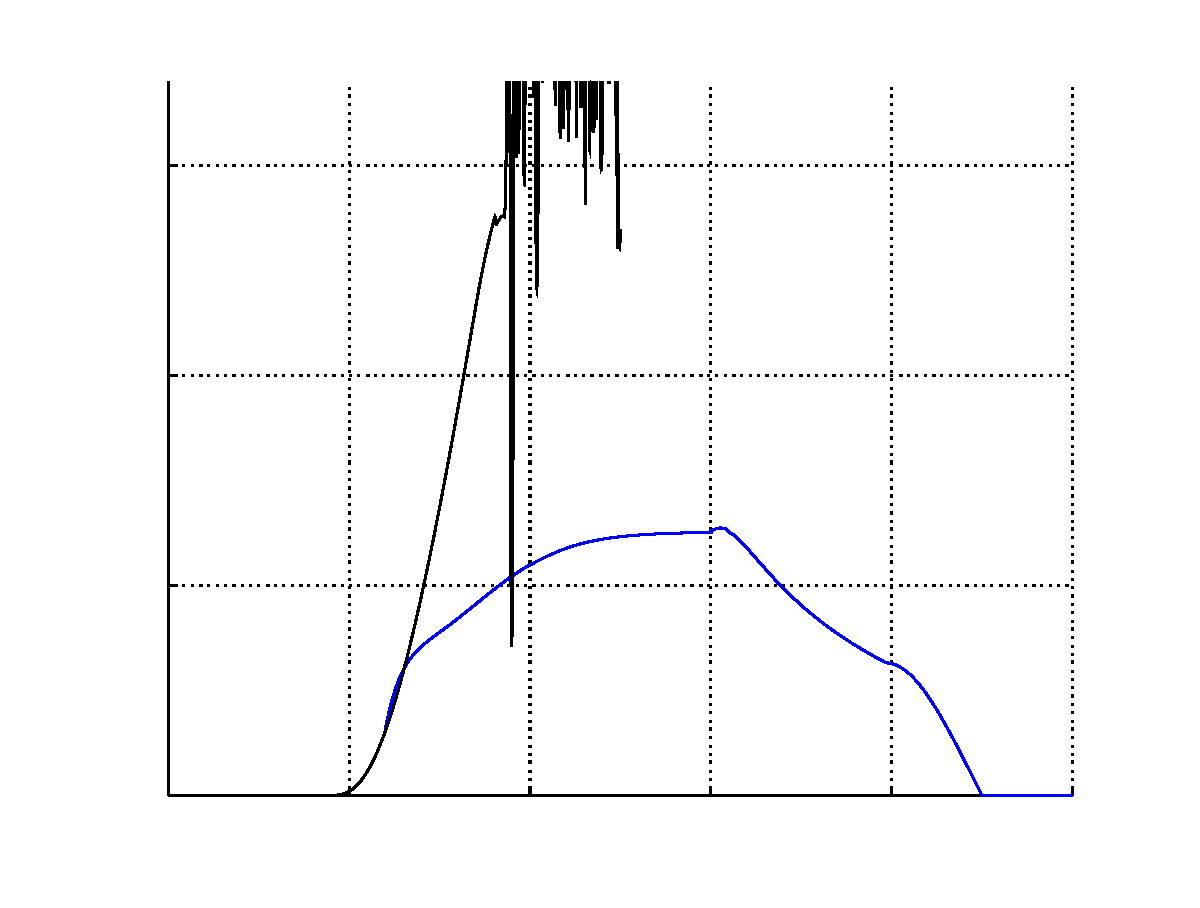
\includegraphics[trim=0  0  0  0,clip,scale=0.6]{test_17_23_force-inc}
\end{picture}%
\begin{picture}(560, 420)(0,0)
\fontsize{11}{0}
\selectfont\put(72.8,41.1956){\makebox(0,0)[t]{\textcolor[rgb]{0,0,0}{{0}}}}
\fontsize{11}{0}
\selectfont\put(159.6,41.1956){\makebox(0,0)[t]{\textcolor[rgb]{0,0,0}{{5}}}}
\fontsize{11}{0}
\selectfont\put(246.4,41.1956){\makebox(0,0)[t]{\textcolor[rgb]{0,0,0}{{10}}}}
\fontsize{11}{0}
\selectfont\put(333.2,41.1956){\makebox(0,0)[t]{\textcolor[rgb]{0,0,0}{{15}}}}
\fontsize{11}{0}
\selectfont\put(420,41.1956){\makebox(0,0)[t]{\textcolor[rgb]{0,0,0}{{20}}}}
\fontsize{11}{0}
\selectfont\put(506.8,41.1956){\makebox(0,0)[t]{\textcolor[rgb]{0,0,0}{{25}}}}
\fontsize{11}{0}
\selectfont\put(67.8,46.2){\makebox(0,0)[r]{\textcolor[rgb]{0,0,0}{{0}}}}
\fontsize{11}{0}
\selectfont\put(67.8,146.876){\makebox(0,0)[r]{\textcolor[rgb]{0,0,0}{{50}}}}
\fontsize{11}{0}
\selectfont\put(67.8,247.553){\makebox(0,0)[r]{\textcolor[rgb]{0,0,0}{{100}}}}
\fontsize{11}{0}
\selectfont\put(67.8,348.229){\makebox(0,0)[r]{\textcolor[rgb]{0,0,0}{{150}}}}
\fontsize{11}{0}
\selectfont\put(289.8,25.1956){\makebox(0,0)[t]{\textcolor[rgb]{0,0,0}{{simulation time $[s]$}}}}
\fontsize{11}{0}
\selectfont\put(39.8,217.35){\rotatebox{90}{\makebox(0,0)[b]{\textcolor[rgb]{0,0,0}{{left hand contact force $\force_{0,\MT{lh}}$ $[N]$}}}}}
\end{picture}

            \subcaption{
                Norms of the optional left hand contact forces. Force shown in
                solid blue line corresponds to the controller with the
                capturability constraint. The controller without the
                capturability constraint produces force shown in solid black.
            }
            \label{fig.force_distrib_task_force}
        }
    \end{minipage}
    \begin{minipage}[t]{\textwidth}
        \centering{
            % Title: glps_renderer figure
% Creator: GL2PS 1.3.8, (C) 1999-2012 C. Geuzaine
% For: Octave
% CreationDate: Mon May  9 19:44:29 2016
\setlength{\unitlength}{0.6pt}
\begin{picture}(0,0)
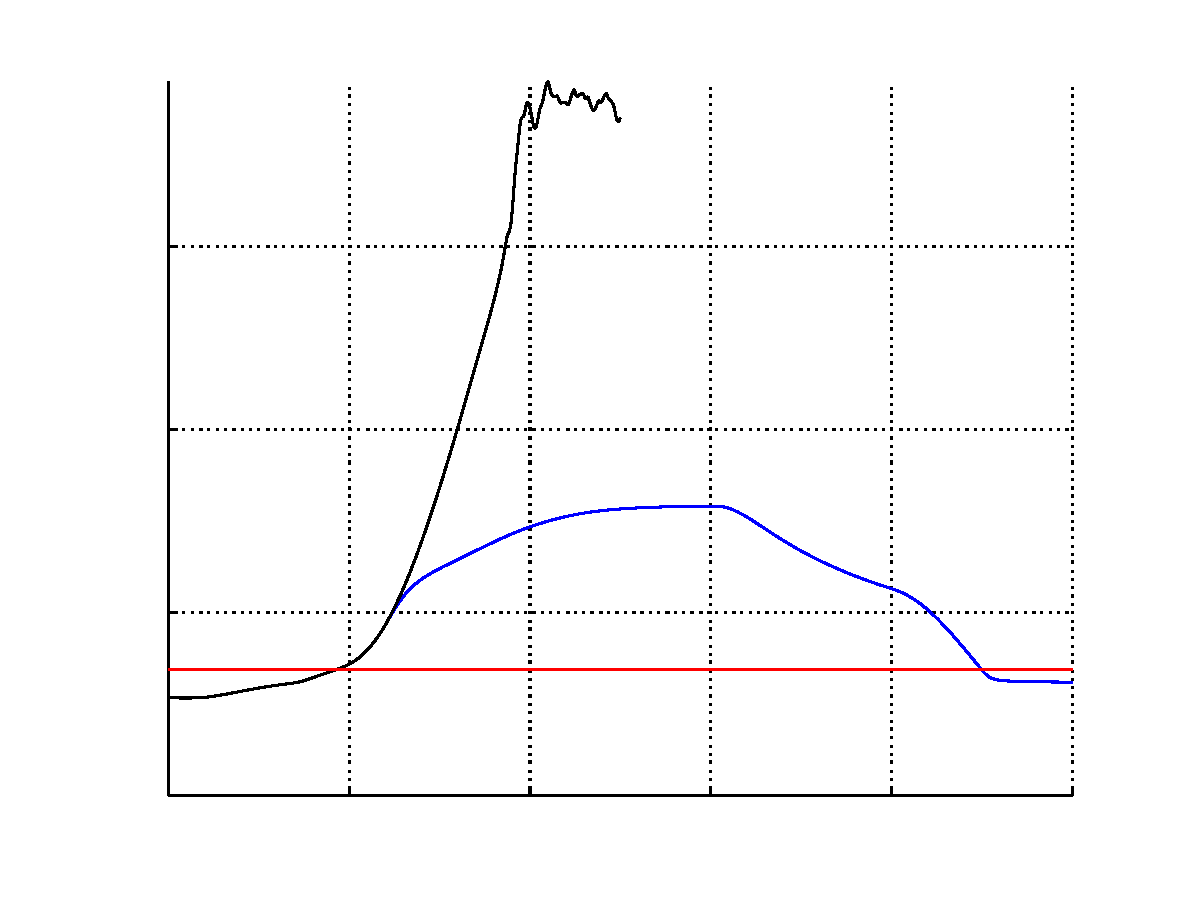
\includegraphics[trim=0  0  0  0,clip,scale=0.6]{test_17_23_com-inc}
\end{picture}%
\begin{picture}(560, 420)(0,0)
\fontsize{11}{0}
\selectfont\put(72.8,41.1956){\makebox(0,0)[t]{\textcolor[rgb]{0,0,0}{{0}}}}
\fontsize{11}{0}
\selectfont\put(159.6,41.1956){\makebox(0,0)[t]{\textcolor[rgb]{0,0,0}{{5}}}}
\fontsize{11}{0}
\selectfont\put(246.4,41.1956){\makebox(0,0)[t]{\textcolor[rgb]{0,0,0}{{10}}}}
\fontsize{11}{0}
\selectfont\put(333.2,41.1956){\makebox(0,0)[t]{\textcolor[rgb]{0,0,0}{{15}}}}
\fontsize{11}{0}
\selectfont\put(420,41.1956){\makebox(0,0)[t]{\textcolor[rgb]{0,0,0}{{20}}}}
\fontsize{11}{0}
\selectfont\put(506.8,41.1956){\makebox(0,0)[t]{\textcolor[rgb]{0,0,0}{{25}}}}
\fontsize{11}{0}
\selectfont\put(67.8,46.2){\makebox(0,0)[r]{\textcolor[rgb]{0,0,0}{{0}}}}
\fontsize{11}{0}
\selectfont\put(67.8,134.023){\makebox(0,0)[r]{\textcolor[rgb]{0,0,0}{{0.1}}}}
\fontsize{11}{0}
\selectfont\put(67.8,221.845){\makebox(0,0)[r]{\textcolor[rgb]{0,0,0}{{0.2}}}}
\fontsize{11}{0}
\selectfont\put(67.8,309.668){\makebox(0,0)[r]{\textcolor[rgb]{0,0,0}{{0.3}}}}
\fontsize{11}{0}
\selectfont\put(289.8,25.1956){\makebox(0,0)[t]{\textcolor[rgb]{0,0,0}{{simulation time $[s]$}}}}
\fontsize{11}{0}
\selectfont\put(43.8,217.35){\rotatebox{90}{\makebox(0,0)[b]{\textcolor[rgb]{0,0,0}{{\ac{CoM} position $[m]$}}}}}
\end{picture}

            \subcaption{
                Position of the \ac{CoM} along the $x$ axis. Position indicated
                with solid blue line corresponds to the controller with the
                capturability constraint. Solid black line indicates position of
                the \ac{CoM} produced by the controller without the
                capturability constraint.
            }
            \label{fig.force_distrib_task_com}
        }
    \end{minipage}
    \caption[Optional contact force: reaching task.]{
        Exploitation of the optional hand contact while performing a right hand
        task.
    }
    \label{fig.force_distrib_task_force_com}
\end{figure}


\begin{figure}[!htbp]
    \begin{minipage}[t]{\textwidth}
        \centering{
            % Title: glps_renderer figure
% Creator: GL2PS 1.3.8, (C) 1999-2012 C. Geuzaine
% For: Octave
% CreationDate: Thu Mar 24 00:51:16 2016
\setlength{\unitlength}{0.6pt}
\begin{picture}(0,0)
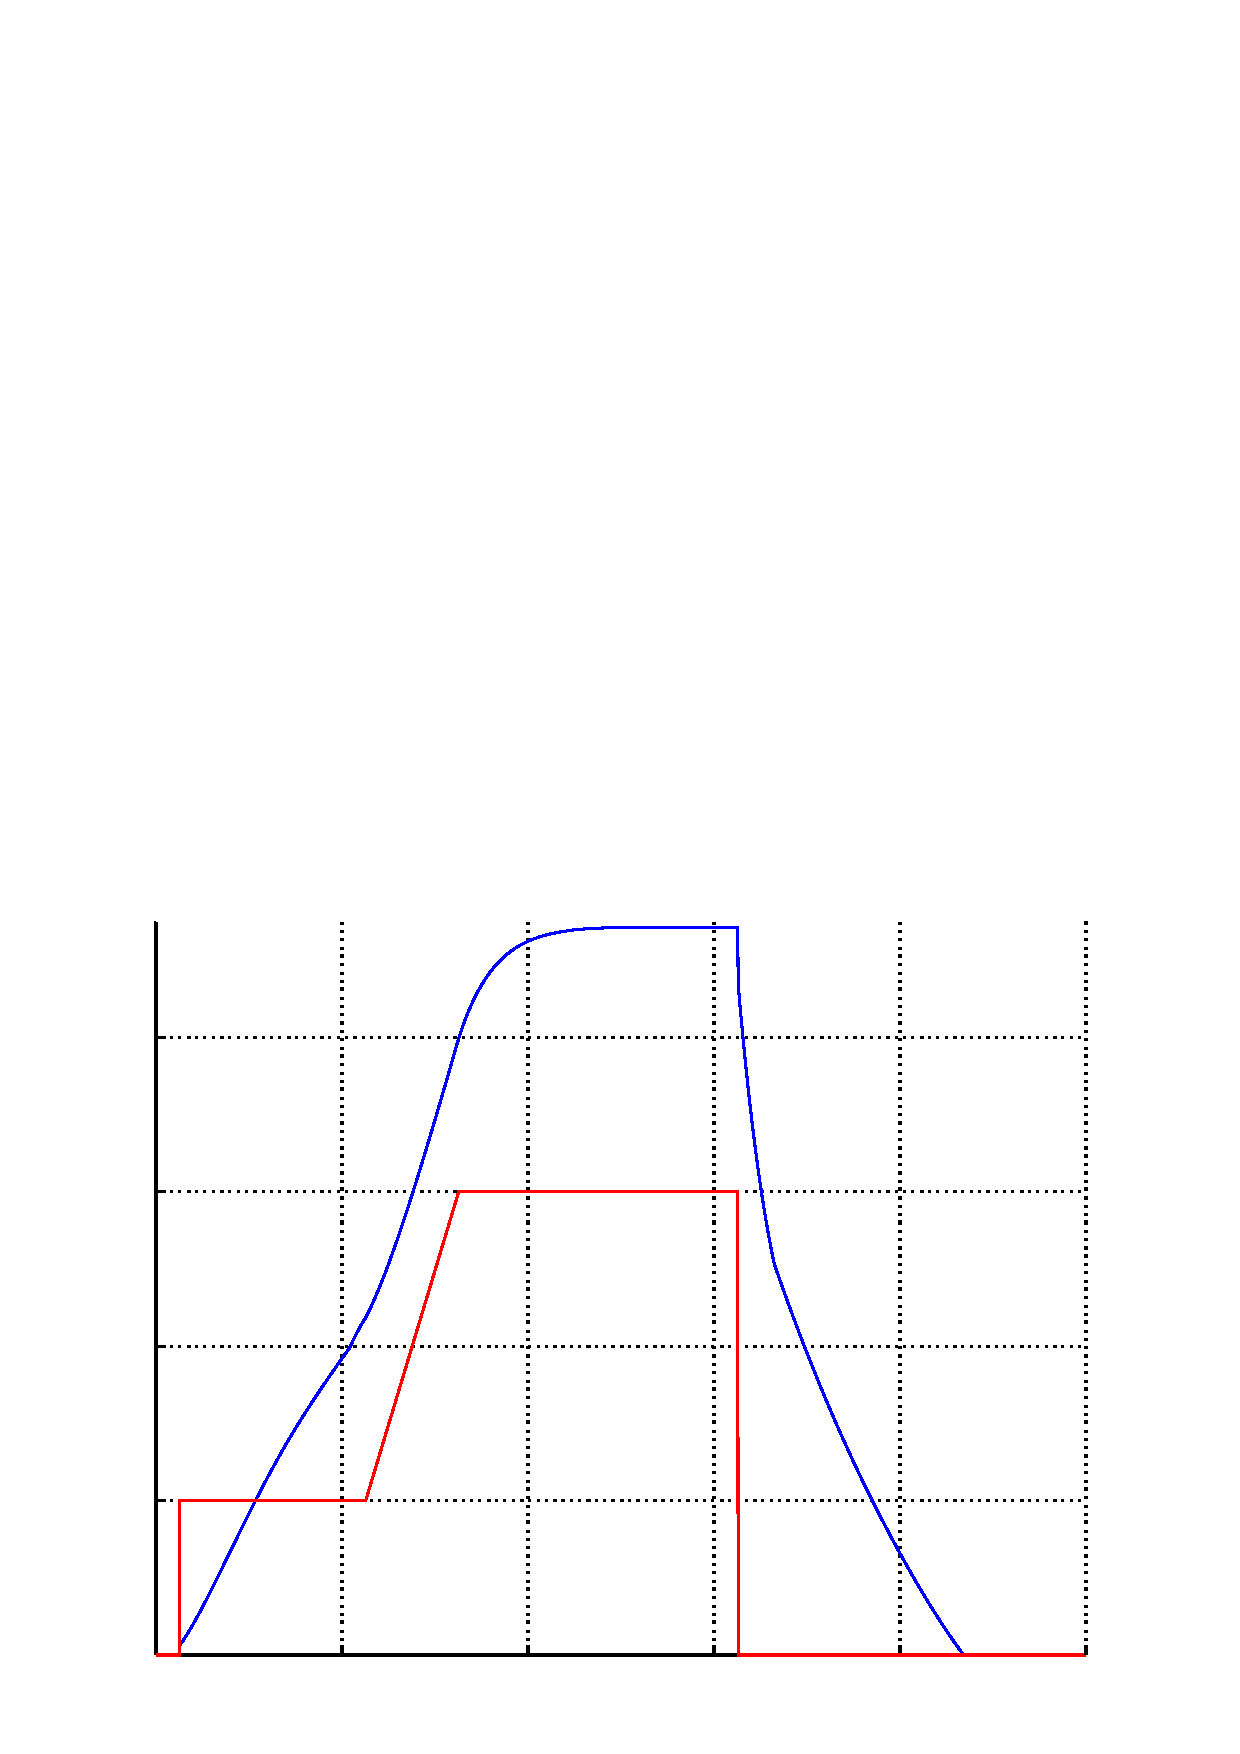
\includegraphics[trim=0  0  0  0,clip,scale=0.6]{test_17_24_force-inc}
\end{picture}%
\begin{picture}(576, 432)(0,0)
\fontsize{11}{0}
\selectfont\put(74.88,42.5189){\makebox(0,0)[t]{\textcolor[rgb]{0,0,0}{{0}}}}
\fontsize{11}{0}
\selectfont\put(164.16,42.5189){\makebox(0,0)[t]{\textcolor[rgb]{0,0,0}{{2}}}}
\fontsize{11}{0}
\selectfont\put(253.44,42.5189){\makebox(0,0)[t]{\textcolor[rgb]{0,0,0}{{4}}}}
\fontsize{11}{0}
\selectfont\put(342.72,42.5189){\makebox(0,0)[t]{\textcolor[rgb]{0,0,0}{{6}}}}
\fontsize{11}{0}
\selectfont\put(432,42.5189){\makebox(0,0)[t]{\textcolor[rgb]{0,0,0}{{8}}}}
\fontsize{11}{0}
\selectfont\put(521.28,42.5189){\makebox(0,0)[t]{\textcolor[rgb]{0,0,0}{{10}}}}
\fontsize{11}{0}
\selectfont\put(69.8755,47.52){\makebox(0,0)[r]{\textcolor[rgb]{0,0,0}{{0}}}}
\fontsize{11}{0}
\selectfont\put(69.8755,121.642){\makebox(0,0)[r]{\textcolor[rgb]{0,0,0}{{20}}}}
\fontsize{11}{0}
\selectfont\put(69.8755,195.764){\makebox(0,0)[r]{\textcolor[rgb]{0,0,0}{{40}}}}
\fontsize{11}{0}
\selectfont\put(69.8755,269.886){\makebox(0,0)[r]{\textcolor[rgb]{0,0,0}{{60}}}}
\fontsize{11}{0}
\selectfont\put(69.8755,344.008){\makebox(0,0)[r]{\textcolor[rgb]{0,0,0}{{80}}}}
\fontsize{11}{0}
\selectfont\put(298.08,26.5189){\makebox(0,0)[t]{\textcolor[rgb]{0,0,0}{{simulation time $[s]$}}}}
\fontsize{11}{0}
\selectfont\put(49.8755,223.56){\rotatebox{90}{\makebox(0,0)[b]{\textcolor[rgb]{0,0,0}{{forces $[N]$}}}}}
\end{picture}

            \subcaption{
                Norms of the optional left hand contact force
                $\V{f}_{0,\MT{lh}}$ (solid blue) and the disturbing external
                force $\V{f}_{\MT{rh}}$ (solid red).
            }
            \label{fig.force_distrib_weight_force}
        }
    \end{minipage}
    \begin{minipage}[t]{\textwidth}
        \centering{
            % Title: glps_renderer figure
% Creator: GL2PS 1.3.8, (C) 1999-2012 C. Geuzaine
% For: Octave
% CreationDate: Thu Mar 24 00:51:17 2016
\setlength{\unitlength}{0.6pt}
\begin{picture}(0,0)
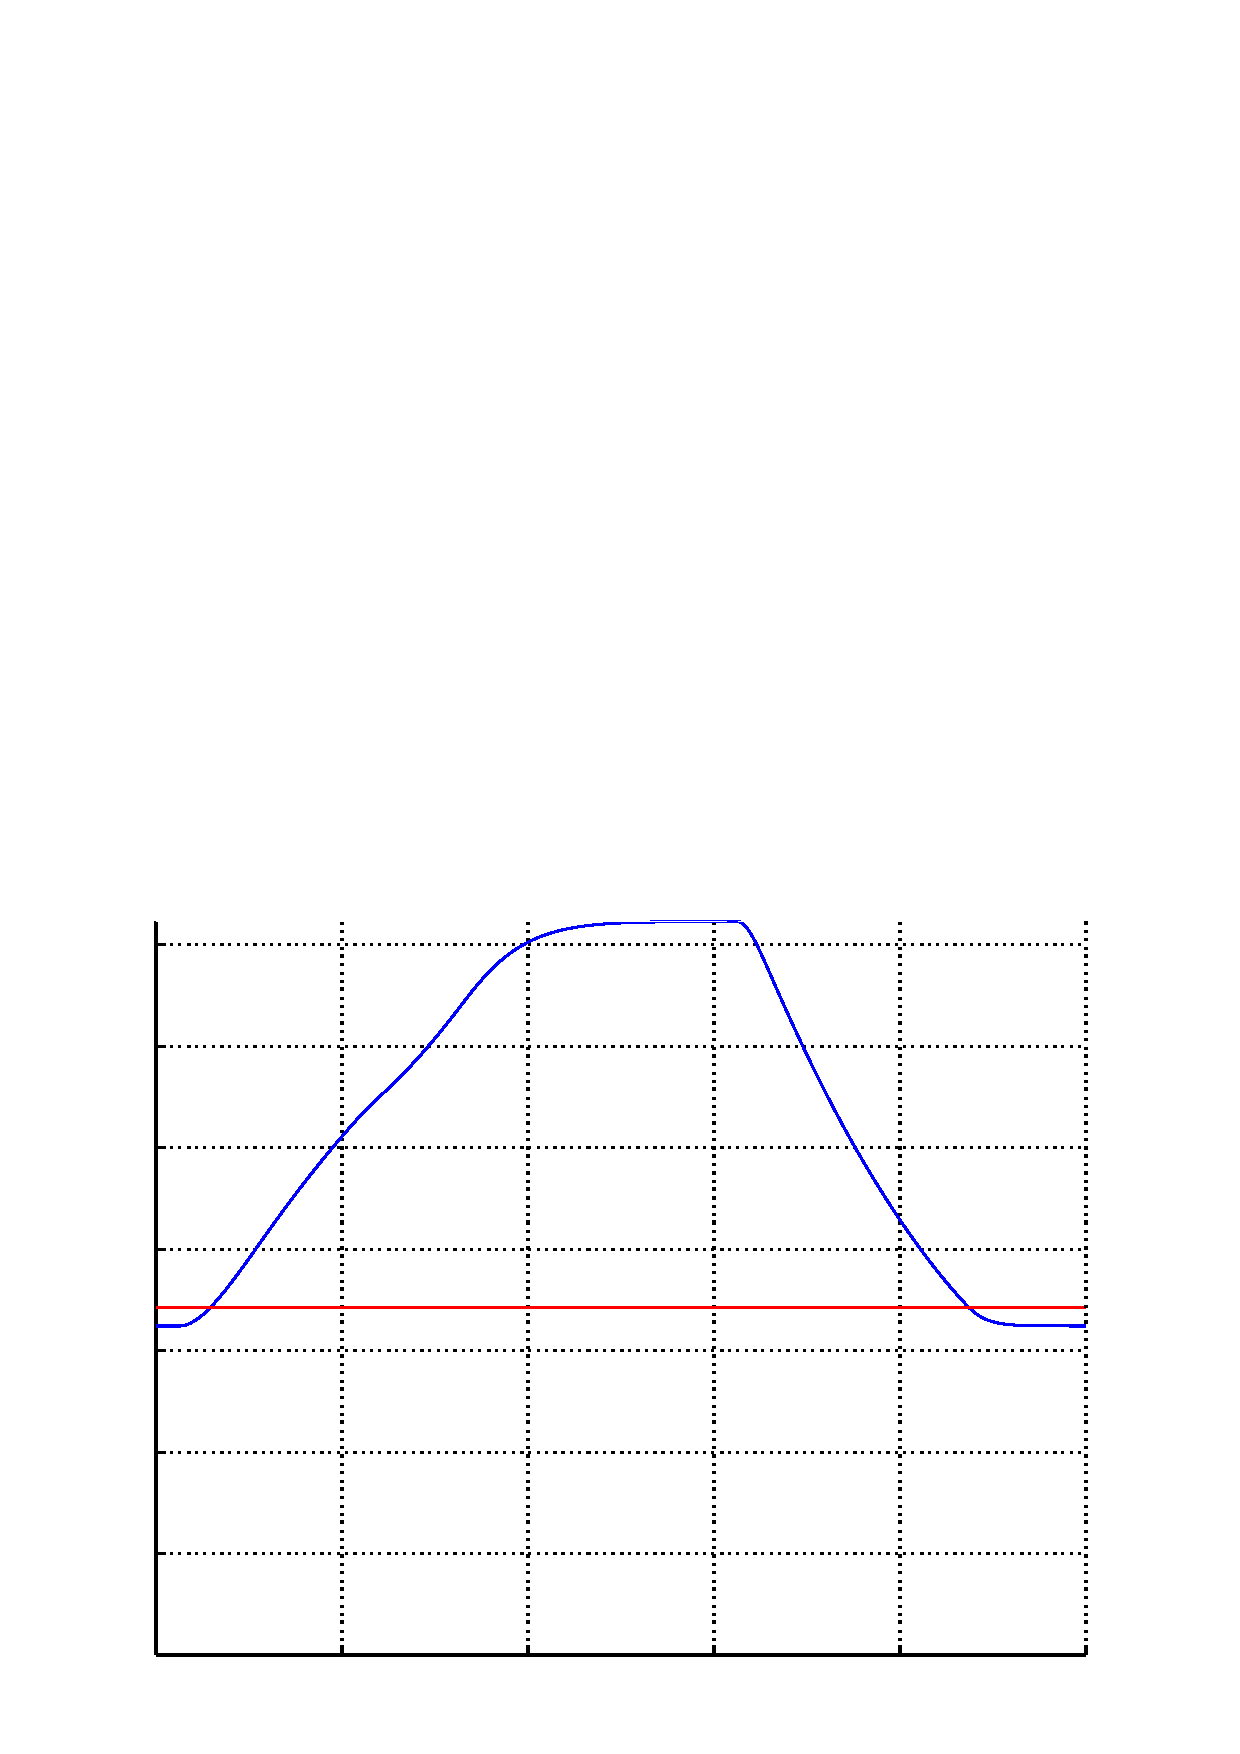
\includegraphics[trim=0  0  0  0,clip,scale=0.6]{test_17_24_com-inc}
\end{picture}%
\begin{picture}(576, 432)(0,0)
\fontsize{11}{0}
\selectfont\put(74.88,42.5189){\makebox(0,0)[t]{\textcolor[rgb]{0,0,0}{{0}}}}
\fontsize{11}{0}
\selectfont\put(164.16,42.5189){\makebox(0,0)[t]{\textcolor[rgb]{0,0,0}{{2}}}}
\fontsize{11}{0}
\selectfont\put(253.44,42.5189){\makebox(0,0)[t]{\textcolor[rgb]{0,0,0}{{4}}}}
\fontsize{11}{0}
\selectfont\put(342.72,42.5189){\makebox(0,0)[t]{\textcolor[rgb]{0,0,0}{{6}}}}
\fontsize{11}{0}
\selectfont\put(432,42.5189){\makebox(0,0)[t]{\textcolor[rgb]{0,0,0}{{8}}}}
\fontsize{11}{0}
\selectfont\put(521.28,42.5189){\makebox(0,0)[t]{\textcolor[rgb]{0,0,0}{{10}}}}
\fontsize{11}{0}
\selectfont\put(69.8755,47.52){\makebox(0,0)[r]{\textcolor[rgb]{0,0,0}{{0}}}}
\fontsize{11}{0}
\selectfont\put(69.8755,96.2139){\makebox(0,0)[r]{\textcolor[rgb]{0,0,0}{{0.02}}}}
\fontsize{11}{0}
\selectfont\put(69.8755,144.908){\makebox(0,0)[r]{\textcolor[rgb]{0,0,0}{{0.04}}}}
\fontsize{11}{0}
\selectfont\put(69.8755,193.602){\makebox(0,0)[r]{\textcolor[rgb]{0,0,0}{{0.06}}}}
\fontsize{11}{0}
\selectfont\put(69.8755,242.295){\makebox(0,0)[r]{\textcolor[rgb]{0,0,0}{{0.08}}}}
\fontsize{11}{0}
\selectfont\put(69.8755,290.989){\makebox(0,0)[r]{\textcolor[rgb]{0,0,0}{{0.1}}}}
\fontsize{11}{0}
\selectfont\put(69.8755,339.683){\makebox(0,0)[r]{\textcolor[rgb]{0,0,0}{{0.12}}}}
\fontsize{11}{0}
\selectfont\put(69.8755,388.377){\makebox(0,0)[r]{\textcolor[rgb]{0,0,0}{{0.14}}}}
\fontsize{11}{0}
\selectfont\put(298.08,26.5189){\makebox(0,0)[t]{\textcolor[rgb]{0,0,0}{{simulation time $[s]$}}}}
\fontsize{11}{0}
\selectfont\put(37.8755,223.56){\rotatebox{90}{\makebox(0,0)[b]{\textcolor[rgb]{0,0,0}{{\ac{CoM} position $[m]$}}}}}
\end{picture}

            \subcaption{
                Position of the \ac{CoM} along the $x$ axis (solid blue) and
                the bound of the foot support area (solid red).
            }
            \label{fig.force_distrib_weight_com}
        }
    \end{minipage}
    \caption[Optional contact force: disturbing force.]{
        Exploitation of the optional hand contact in presence of external
        disturbing force.
    }
    \label{fig.force_distrib_weight_force_com}
\end{figure}



\begin{figure}[!htbp]
    \centering{
        % Title: glps_renderer figure
% Creator: GL2PS 1.3.8, (C) 1999-2012 C. Geuzaine
% For: Octave
% CreationDate: Mon May  9 19:44:35 2016
\setlength{\unitlength}{0.7pt}
\begin{picture}(0,0)
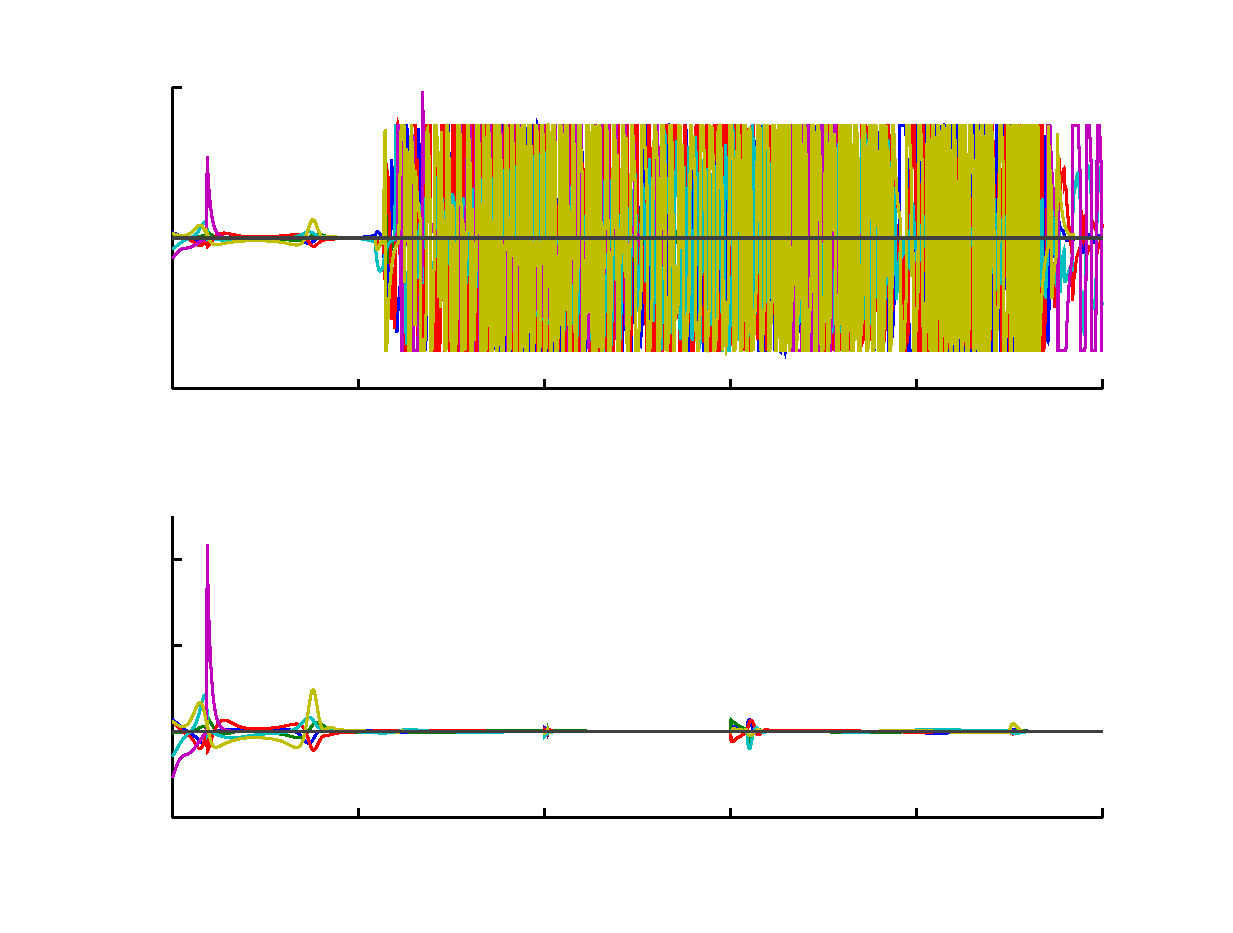
\includegraphics[trim=0  0  0  0,clip,scale=0.7]{test_17_23_joints-inc}
\end{picture}%
\begin{picture}(576, 432)(0,0)
\fontsize{11}{0}
\selectfont\put(74.88,248.382){\makebox(0,0)[t]{\textcolor[rgb]{0,0,0}{{0}}}}
\fontsize{11}{0}
\selectfont\put(164.16,248.382){\makebox(0,0)[t]{\textcolor[rgb]{0,0,0}{{5}}}}
\fontsize{11}{0}
\selectfont\put(253.44,248.382){\makebox(0,0)[t]{\textcolor[rgb]{0,0,0}{{10}}}}
\fontsize{11}{0}
\selectfont\put(342.72,248.382){\makebox(0,0)[t]{\textcolor[rgb]{0,0,0}{{15}}}}
\fontsize{11}{0}
\selectfont\put(432,248.382){\makebox(0,0)[t]{\textcolor[rgb]{0,0,0}{{20}}}}
\fontsize{11}{0}
\selectfont\put(521.28,248.382){\makebox(0,0)[t]{\textcolor[rgb]{0,0,0}{{25}}}}
\fontsize{11}{0}
\selectfont\put(69.8755,253.397){\makebox(0,0)[r]{\textcolor[rgb]{0,0,0}{{-40}}}}
\fontsize{11}{0}
\selectfont\put(69.8755,325.617){\makebox(0,0)[r]{\textcolor[rgb]{0,0,0}{{0}}}}
\fontsize{11}{0}
\selectfont\put(69.8755,397.837){\makebox(0,0)[r]{\textcolor[rgb]{0,0,0}{{40}}}}
\fontsize{11}{0}
\selectfont\put(44.8755,325.617){\rotatebox{90}{\makebox(0,0)[b]{\textcolor[rgb]{0,0,0}{{$\ddq_{\MT{rh}}~[\MT{rad}/s^2]$}}}}}
\fontsize{11}{0}
\selectfont\put(74.88,42.5047){\makebox(0,0)[t]{\textcolor[rgb]{0,0,0}{{0}}}}
\fontsize{11}{0}
\selectfont\put(164.16,42.5047){\makebox(0,0)[t]{\textcolor[rgb]{0,0,0}{{5}}}}
\fontsize{11}{0}
\selectfont\put(253.44,42.5047){\makebox(0,0)[t]{\textcolor[rgb]{0,0,0}{{10}}}}
\fontsize{11}{0}
\selectfont\put(342.72,42.5047){\makebox(0,0)[t]{\textcolor[rgb]{0,0,0}{{15}}}}
\fontsize{11}{0}
\selectfont\put(432,42.5047){\makebox(0,0)[t]{\textcolor[rgb]{0,0,0}{{20}}}}
\fontsize{11}{0}
\selectfont\put(521.28,42.5047){\makebox(0,0)[t]{\textcolor[rgb]{0,0,0}{{25}}}}
\fontsize{11}{0}
\selectfont\put(69.8755,47.52){\makebox(0,0)[r]{\textcolor[rgb]{0,0,0}{{-10}}}}
\fontsize{11}{0}
\selectfont\put(69.8755,88.7886){\makebox(0,0)[r]{\textcolor[rgb]{0,0,0}{{0}}}}
\fontsize{11}{0}
\selectfont\put(69.8755,130.057){\makebox(0,0)[r]{\textcolor[rgb]{0,0,0}{{10}}}}
\fontsize{11}{0}
\selectfont\put(69.8755,171.326){\makebox(0,0)[r]{\textcolor[rgb]{0,0,0}{{20}}}}
\fontsize{11}{0}
\selectfont\put(298.08,26.5047){\makebox(0,0)[t]{\textcolor[rgb]{0,0,0}{{simulation time $[s]$}}}}
\fontsize{11}{0}
\selectfont\put(44.8755,119.74){\rotatebox{90}{\makebox(0,0)[b]{\textcolor[rgb]{0,0,0}{{$\ddq_{\MT{rh}}~[\MT{rad}/s^2]$}}}}}
\end{picture}

        \caption[Chattering of the joint accelerations.]{
            Accelerations of the right arm joints without regularization (top)
            and with it (bottom).
        }
        \label{fig.chattering}
    }
\end{figure}



\begin{figure}[!htbp]
    \centering{
        % Title: glps_renderer figure
% Creator: GL2PS 1.3.8, (C) 1999-2012 C. Geuzaine
% For: Octave
% CreationDate: Mon May  9 19:44:34 2016
\setlength{\unitlength}{0.7pt}
\begin{picture}(0,0)
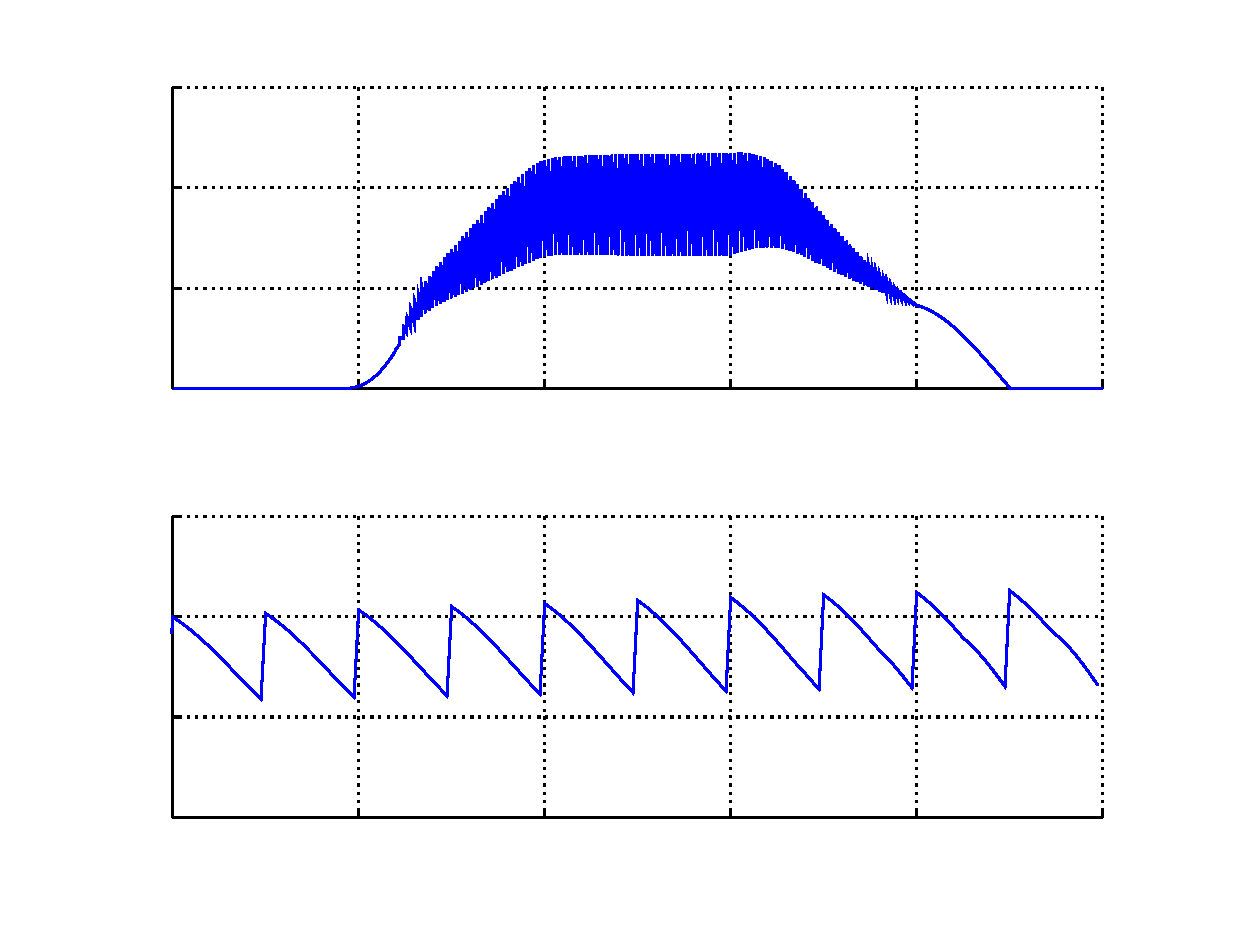
\includegraphics[trim=0  0  0  0,clip,scale=0.7]{test_17_23_badmpc_force-inc}
\end{picture}%
\begin{picture}(576, 432)(0,0)
\fontsize{11}{0}
\selectfont\put(74.88,248.382){\makebox(0,0)[t]{\textcolor[rgb]{0,0,0}{{0}}}}
\fontsize{11}{0}
\selectfont\put(164.16,248.382){\makebox(0,0)[t]{\textcolor[rgb]{0,0,0}{{5}}}}
\fontsize{11}{0}
\selectfont\put(253.44,248.382){\makebox(0,0)[t]{\textcolor[rgb]{0,0,0}{{10}}}}
\fontsize{11}{0}
\selectfont\put(342.72,248.382){\makebox(0,0)[t]{\textcolor[rgb]{0,0,0}{{15}}}}
\fontsize{11}{0}
\selectfont\put(432,248.382){\makebox(0,0)[t]{\textcolor[rgb]{0,0,0}{{20}}}}
\fontsize{11}{0}
\selectfont\put(521.28,248.382){\makebox(0,0)[t]{\textcolor[rgb]{0,0,0}{{25}}}}
\fontsize{11}{0}
\selectfont\put(69.8755,253.397){\makebox(0,0)[r]{\textcolor[rgb]{0,0,0}{{0}}}}
\fontsize{11}{0}
\selectfont\put(69.8755,301.544){\makebox(0,0)[r]{\textcolor[rgb]{0,0,0}{{40}}}}
\fontsize{11}{0}
\selectfont\put(69.8755,349.691){\makebox(0,0)[r]{\textcolor[rgb]{0,0,0}{{80}}}}
\fontsize{11}{0}
\selectfont\put(69.8755,397.837){\makebox(0,0)[r]{\textcolor[rgb]{0,0,0}{{120}}}}
\fontsize{11}{0}
\selectfont\put(41.8755,325.617){\rotatebox{90}{\makebox(0,0)[b]{\textcolor[rgb]{0,0,0}{{$\force_{0,\MT{lh}}$ $[N]$}}}}}
\fontsize{11}{0}
\selectfont\put(74.88,42.5047){\makebox(0,0)[t]{\textcolor[rgb]{0,0,0}{{9}}}}
\fontsize{11}{0}
\selectfont\put(164.16,42.5047){\makebox(0,0)[t]{\textcolor[rgb]{0,0,0}{{9.2}}}}
\fontsize{11}{0}
\selectfont\put(253.44,42.5047){\makebox(0,0)[t]{\textcolor[rgb]{0,0,0}{{9.4}}}}
\fontsize{11}{0}
\selectfont\put(342.72,42.5047){\makebox(0,0)[t]{\textcolor[rgb]{0,0,0}{{9.6}}}}
\fontsize{11}{0}
\selectfont\put(432,42.5047){\makebox(0,0)[t]{\textcolor[rgb]{0,0,0}{{9.8}}}}
\fontsize{11}{0}
\selectfont\put(521.28,42.5047){\makebox(0,0)[t]{\textcolor[rgb]{0,0,0}{{10}}}}
\fontsize{11}{0}
\selectfont\put(69.8757,47.52){\makebox(0,0)[r]{\textcolor[rgb]{0,0,0}{{0}}}}
\fontsize{11}{0}
\selectfont\put(69.8757,95.6667){\makebox(0,0)[r]{\textcolor[rgb]{0,0,0}{{40}}}}
\fontsize{11}{0}
\selectfont\put(69.8757,143.813){\makebox(0,0)[r]{\textcolor[rgb]{0,0,0}{{80}}}}
\fontsize{11}{0}
\selectfont\put(69.8757,191.96){\makebox(0,0)[r]{\textcolor[rgb]{0,0,0}{{120}}}}
\fontsize{11}{0}
\selectfont\put(298.08,26.5047){\makebox(0,0)[t]{\textcolor[rgb]{0,0,0}{{simulation time $[s]$}}}}
\fontsize{11}{0}
\selectfont\put(41.8756,119.74){\rotatebox{90}{\makebox(0,0)[b]{\textcolor[rgb]{0,0,0}{{$\force_{0,\MT{lh}}$ $[N]$}}}}}
\end{picture}

        \caption[Periodic variations in the norm of the optional contact force.]{
            Norm of the optional left hand contact force when the first
            sampling interval is reduced at each control iteration.
        }
        \label{fig.subsampling}
    }
\end{figure}




%%%%%%%%%%%%%%%%%%%%%%%%%%%%%%%%%%%%%%%%%%%%%%%%%%%%%%%%%%%%%%%%%%%%%%%%%%%%%%%%
\subsection{Conclusion}\label{sec.force_conclusion}

An interesting property of the constructed controller is that the decision to
apply the optional contact force is taken automatically based on the current
state and tasks. Hence, there is no need for planning and tuning of contact
timings, which are recognized as a significant drawback of approximate linear
models \cite{Audren2014iros}. On the other hand, the considered setting is very
limited: the contact positions are known and fixed in advance. Extensibility of
the approach to more general situations is to be investigated.


One potential application of the controller could be evaluation of necessity of
an optional contact for balance preservation in the future. For example, when
the robot is pushed, the controller may decide if using an additional hand
contact with a wall at some time $t$ in the future would be necessary to avoid
a fall. If so, an appropriate task can be triggered to move the hand towards
the wall.


We believe that the current primary obstacle for adoption of the proposed
approach is the lack of numerical tools, which can solve hierarchies both
efficiently and accurately. The size of \cref{hr.mmpc_force} makes its solution
with a sequence of \acs{QP}s impractical. At the same time, the existing
specialized solvers for hierarchies, \sn{LexLS} \cite{Dimitrov2015preprint} and
\sn{SOTH} \cite{Escande2014ijrr, SOTHsite}, provide very limited mechanisms for
coping with the numerical problems near singularities discussed in
\cref{sec.force_results}. Since singularities commonly arise due to conflicts
in hierarchies, it is necessary to develop and extend these mechanisms in order
to maximally benefit from prioritization. For example, it is desirable to have
regularization with general equality objective with automatic selection of the
regularization factor (see \cref{sec.regularization}).



%%%%%%%%%%%%%%%%%%%%%%%%%%%%%%%%%%%%%%%%%%%%%%%%%%%%%%%%%%%%%%%%%%%%%%%%%%%%%%%%
%%%%%%%%%%%%%%%%%%%%%%%%%%%%%%%%%%%%%%%%%%%%%%%%%%%%%%%%%%%%%%%%%%%%%%%%%%%%%%%%
%%%%%%%%%%%%%%%%%%%%%%%%%%%%%%%%%%%%%%%%%%%%%%%%%%%%%%%%%%%%%%%%%%%%%%%%%%%%%%%%
\section{Collaborations}\label{sec.collaboration_results}

A substantial part of the work covered by the present thesis was performed in
collaboration with other doctoral and master students from different research
institutes. The author's contribution to the collaborative works is briefly
outlined in the following subsections.


%%%%%%%%%%%%%%%%%%%%%%%%%%%%%%%%%%%%%%%%%%%%%%%%%%%%%%%%%%%%%%%%%%%%%%%%%%%%%%%%
\subsection{Walking with nonplanar CoM motion}\label{sec.3d_walk}

One of the recurring assumptions made in the construction of linear approximate
models of humanoid robots is that the \ac{CoM} motion is constrained to a plane
(see \cref{ass.fixed_z_coordinate} in \cref{sec.linear_approx_models}). This
limitation is particularly inconvenient when the robot has to walk on uneven
terrain, \IE, when walking up and down stairs. Moreover, even walking on a flat
ground with planar \ac{CoM} motion is unnatural and energy inefficient in
comparison with humans. This issue was addressed in the Master's thesis of
Camille Brasseur, who was, to some extend, co-advised by the author.


Camille's work resulted in the development of an approximate model
\cite{Brasseur2015thesis}, which enables nonplanar motion of the \ac{CoM} at
the price of a larger number of constraints, as indicated in
\cref{sec.point_mass_nonplanar} of this thesis. The obtained model was employed
by Camille in the implementation of an \ac{MPC} scheme for the generation of
walking motions on flat and uneven ground. Since this \ac{MPC} scheme was not
integrated in an \ac{MMPC} controller, the author developed a simple whole body
inverse dynamics controller based on \cref{hr.wbc_controller} for tracking the
generated \ac{CoM} and foot trajectories. The whole body controller was used to
demonstrate the validity of the approach using a simulated \sn{HRP-2} robot.
Snapshots of a simulated walk on stairs are given in \cref{fig.stairs_walk}.
This joint work led to a publication in a conference proceedings
\cite{Brasseur2015humanoids}. Also, the results with detailed derivations were
reported in the corresponding Master's thesis \cite{Brasseur2015thesis}.


%
\begin{figure}[!htb]
    \centering{
        % Title: glps_renderer figure
% Creator: GL2PS 1.3.8, (C) 1999-2012 C. Geuzaine
% For: Octave
% CreationDate: Wed Jun  8 12:43:33 2016
\setlength{\unitlength}{0.9pt}
\begin{picture}(0,0)
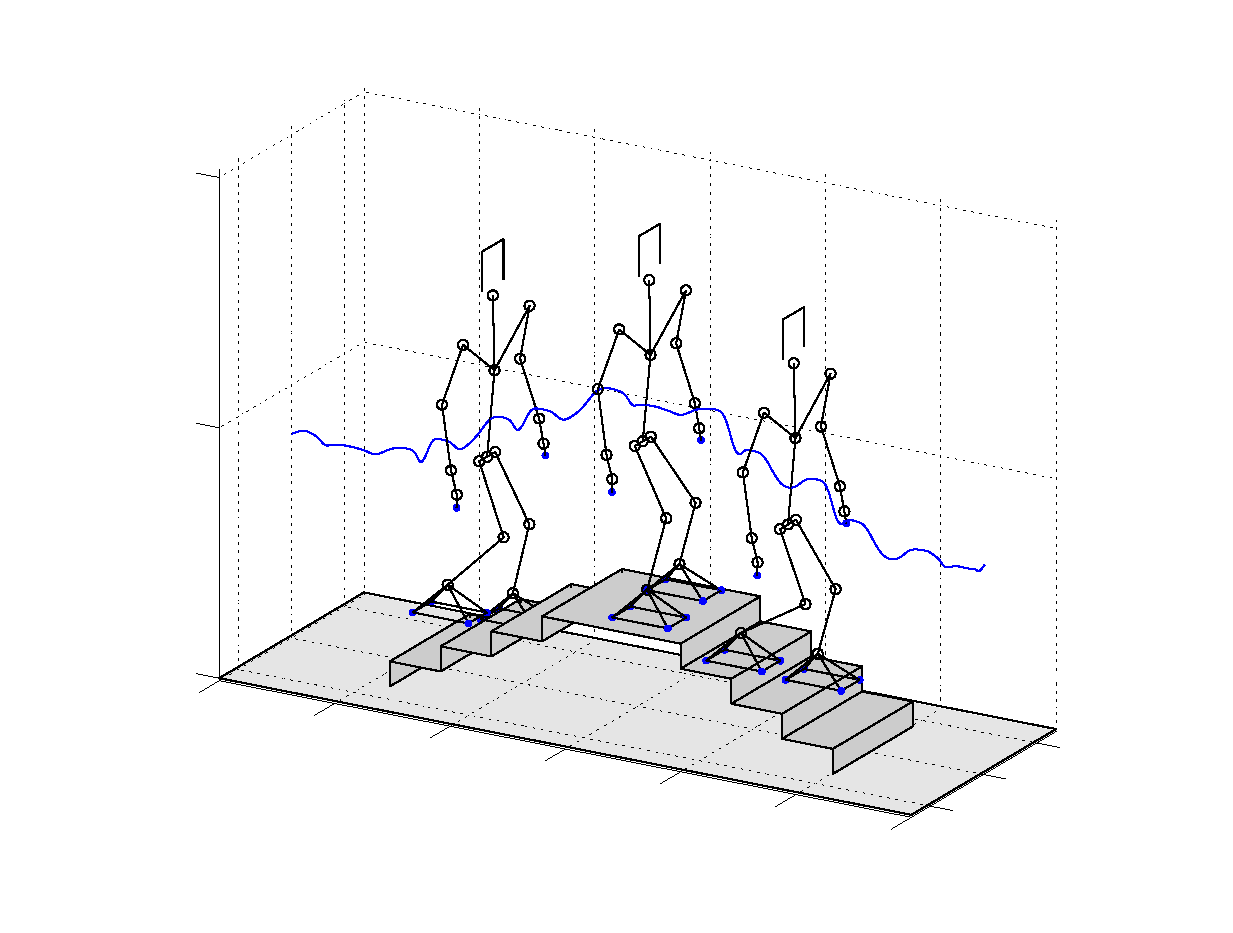
\includegraphics[trim=60  30  50   5,clip,scale=0.9]{test_16_16_robot_on_stairs-inc}
\end{picture}%
\begin{picture}(466, 397)(60,30)
\fontsize{10}{0}
\selectfont\put(81.3775,117.452){\makebox(0,0)[br]{\textcolor[rgb]{0,0,0}{{0}}}}
\fontsize{10}{0}
\selectfont\put(81.3775,237.605){\makebox(0,0)[br]{\textcolor[rgb]{0,0,0}{{1}}}}
\fontsize{10}{0}
\selectfont\put(81.3775,357.759){\makebox(0,0)[br]{\textcolor[rgb]{0,0,0}{{2}}}}
\fontsize{10}{0}
\selectfont\put(83.2472,104.831){\makebox(0,0)[tr]{\textcolor[rgb]{0,0,0}{{0}}}}
\fontsize{10}{0}
\selectfont\put(138.614,93.8979){\makebox(0,0)[tr]{\textcolor[rgb]{0,0,0}{{0.5}}}}
\fontsize{10}{0}
\selectfont\put(209.382,299.759){\makebox(0,0)[l]{\textcolor[rgb]{0,0,0}{{(1)}}}}
\fontsize{10}{0}
\selectfont\put(193.981,82.9648){\makebox(0,0)[tr]{\textcolor[rgb]{0,0,0}{{1}}}}
\fontsize{10}{0}
\selectfont\put(249.348,72.0317){\makebox(0,0)[tr]{\textcolor[rgb]{0,0,0}{{1.5}}}}
\fontsize{10}{0}
\selectfont\put(281.359,309.577){\makebox(0,0)[l]{\textcolor[rgb]{0,0,0}{{(2)}}}}
\fontsize{10}{0}
\selectfont\put(304.716,61.0986){\makebox(0,0)[tr]{\textcolor[rgb]{0,0,0}{{2}}}}
\fontsize{10}{0}
\selectfont\put(360.083,50.1655){\makebox(0,0)[tr]{\textcolor[rgb]{0,0,0}{{2.5}}}}
\fontsize{10}{0}
\selectfont\put(415.45,39.2325){\makebox(0,0)[tr]{\textcolor[rgb]{0,0,0}{{3}}}}
\fontsize{10}{0}
\selectfont\put(454.357,49.7542){\makebox(0,0)[tl]{\textcolor[rgb]{0,0,0}{{-0.4}}}}
\fontsize{10}{0}
\selectfont\put(479.93,64.9035){\makebox(0,0)[tl]{\textcolor[rgb]{0,0,0}{{0}}}}
\fontsize{10}{0}
\selectfont\put(505.503,80.0528){\makebox(0,0)[tl]{\textcolor[rgb]{0,0,0}{{0.4}}}}
\fontsize{10}{0}
\selectfont\put(353.336,271.333){\makebox(0,0)[l]{\textcolor[rgb]{0,0,0}{{(3)}}}}
\end{picture}

        \caption[Robot walking up and down stairs.]{
            Robot walking up and down stairs. Sequence of the snapshots is
            indicated by the numbers. Blue curve indicates nonplanar trajectory
            of the \ac{CoM}.
        }
        \label{fig.stairs_walk}
    }
\end{figure}
%


%%%%%%%%%%%%%%%%%%%%%%%%%%%%%%%%%%%%%%%%%%%%%%%%%%%%%%%%%%%%%%%%%%%%%%%%%%%%%%%%
\subsection{Time-optimal control of industrial manipulators}\label{sec.time_opt}

The idea of time-optimal control using the temporal task prioritization in an
\acs{MPC} problem, as described in \cref{sec.time_optimal_mpc}, was proposed by
the author to another doctoral student, Saed Al Homsi, who performed research
in time-optimal control of industrial manipulators. One of the goals of Saed's
work was to reduce involvement of humans in deployment of industrial robots
operating in a shared environment. One of the problems, which must be faced in
such setups, is collision avoidance between the robots (see \cref{fig.cobra}).
This can be achieved by designing an \ac{MPC} scheme with appropriate
constraints on positions of the links of the manipulator. At the same time,
addition of task prioritization in this \ac{MPC} problem allows for
time-optimal behavior, which is valuable in industrial applications. The
obtained \ac{PLLS} optimization problem can be solved using \sn{LexLS} or
another specialized solver.

Based on the proposed approach to time-optimal control, Saed developed a
real-time controller for Adept Cobra \acs{SCARA} manipulators \cite{ADEPTsite}
and validated it on real robots in the experimental setup visualized in
\cref{fig.cobra}. Results of the experiments with additional simulations and
overview of the concept were published in \cite{alHomsi2016icra}, an interested
reader can find further details in Saed's dissertation
\cite{alHomsi2016thesis}.


%
\begin{figure}[!htb]
    \begin{minipage}[t]{0.49\textwidth}
        \centering{
            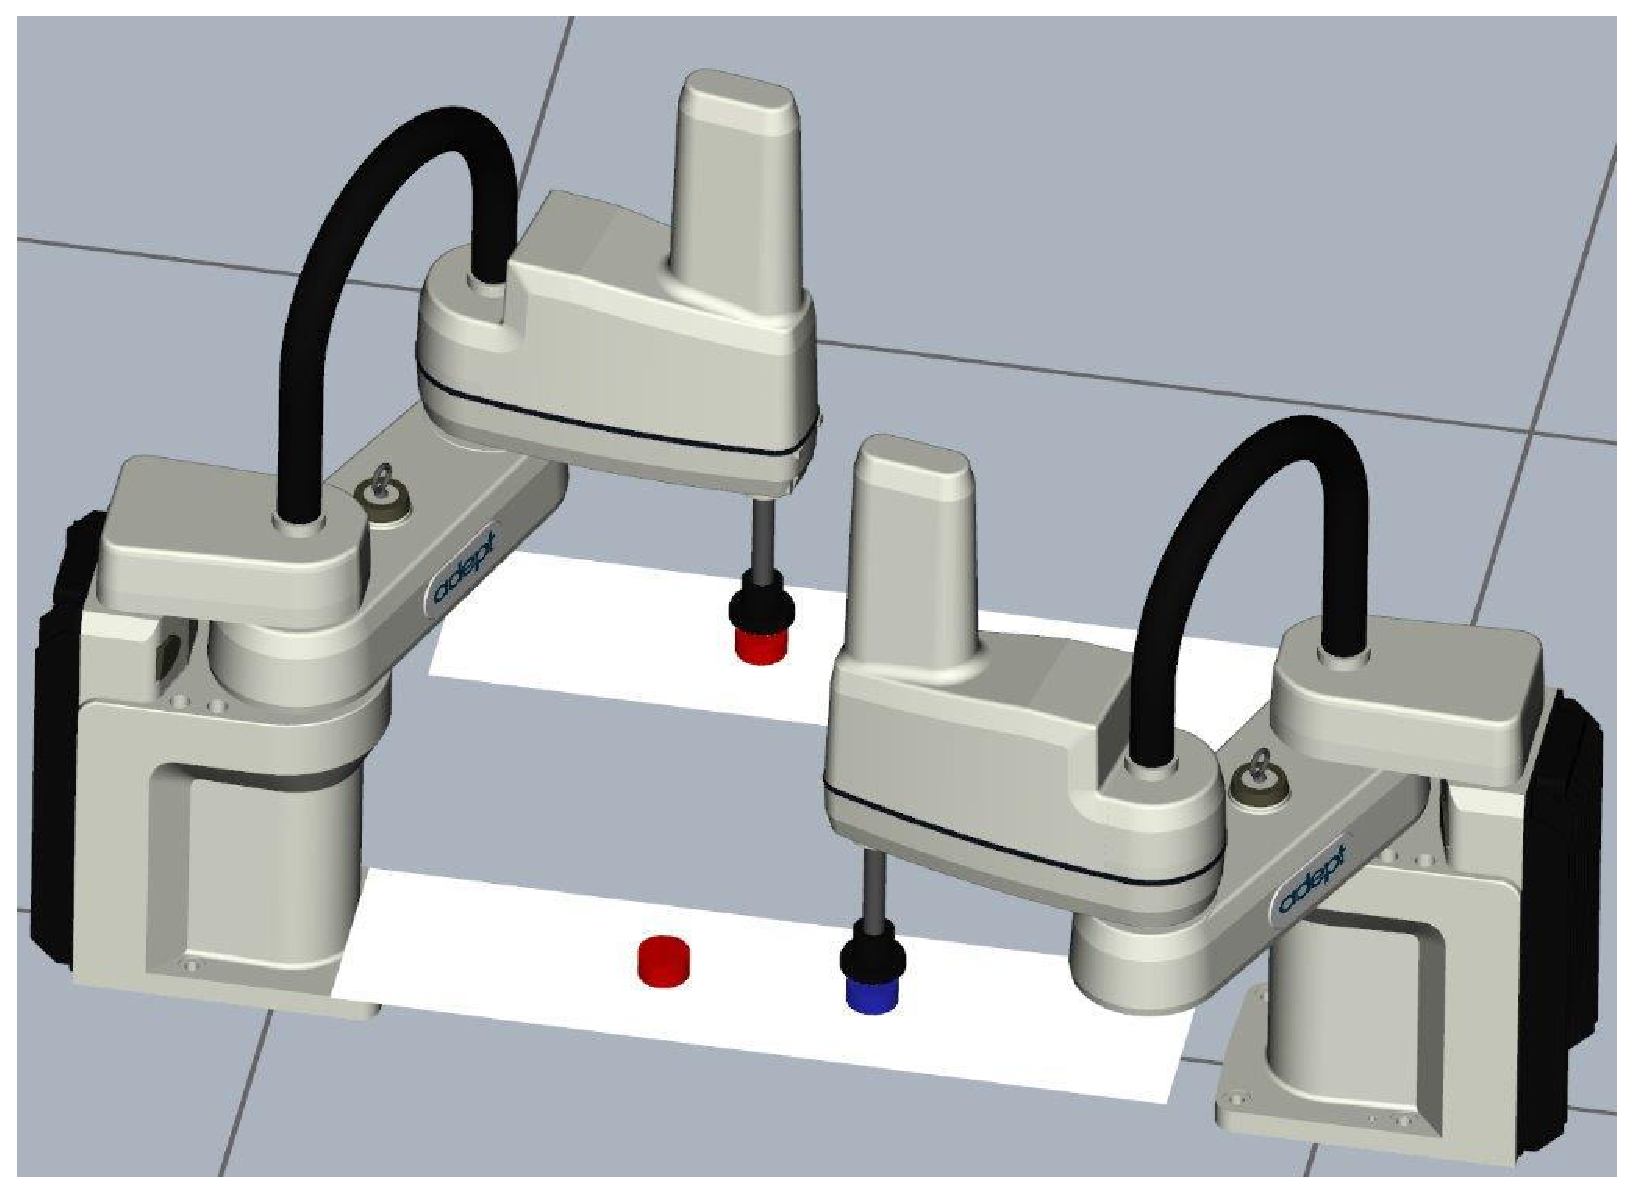
\includegraphics[scale=0.25]{cobra_1.eps}\\
            (1)
            \vspace{0.2cm}
        }
    \end{minipage}
    \hfill
    \begin{minipage}[t]{0.49\textwidth}
        \centering{
            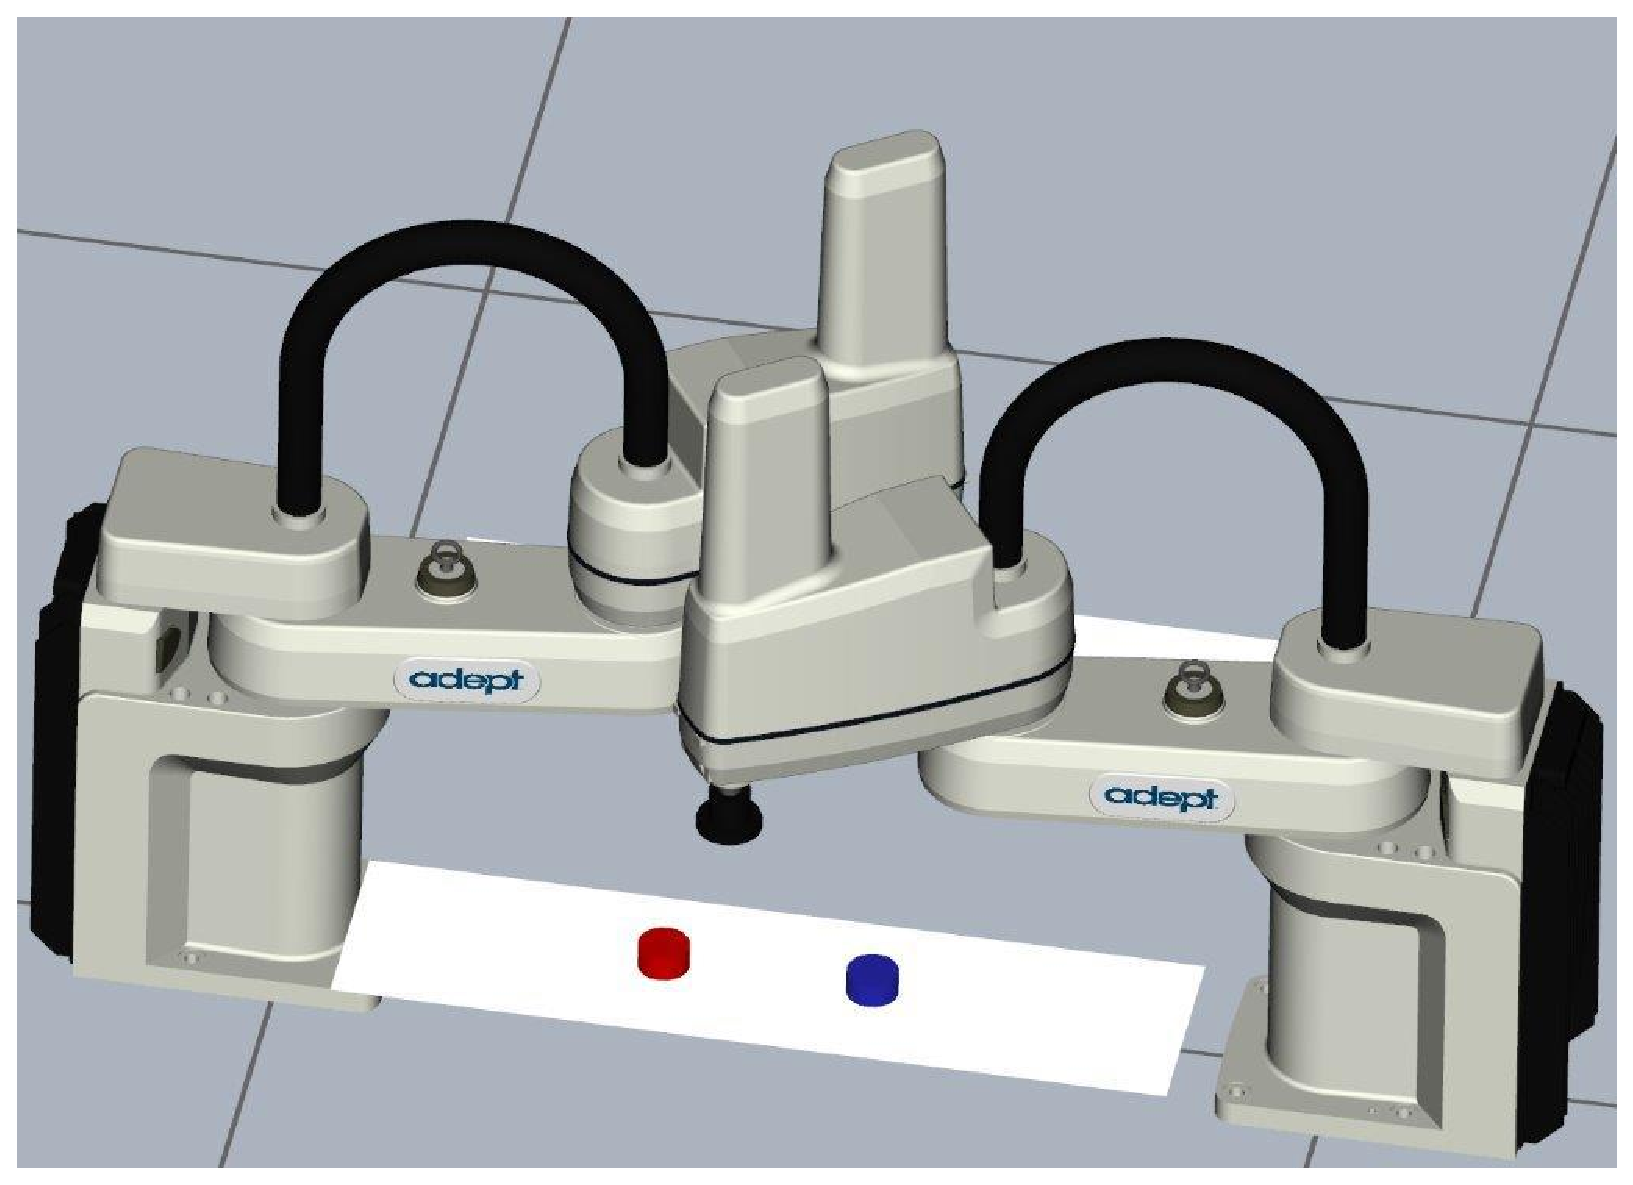
\includegraphics[scale=0.25]{cobra_2.eps}\\
            (2)
            \vspace{0.2cm}
        }
    \end{minipage}
    \begin{minipage}[t]{0.49\textwidth}
        \centering{
            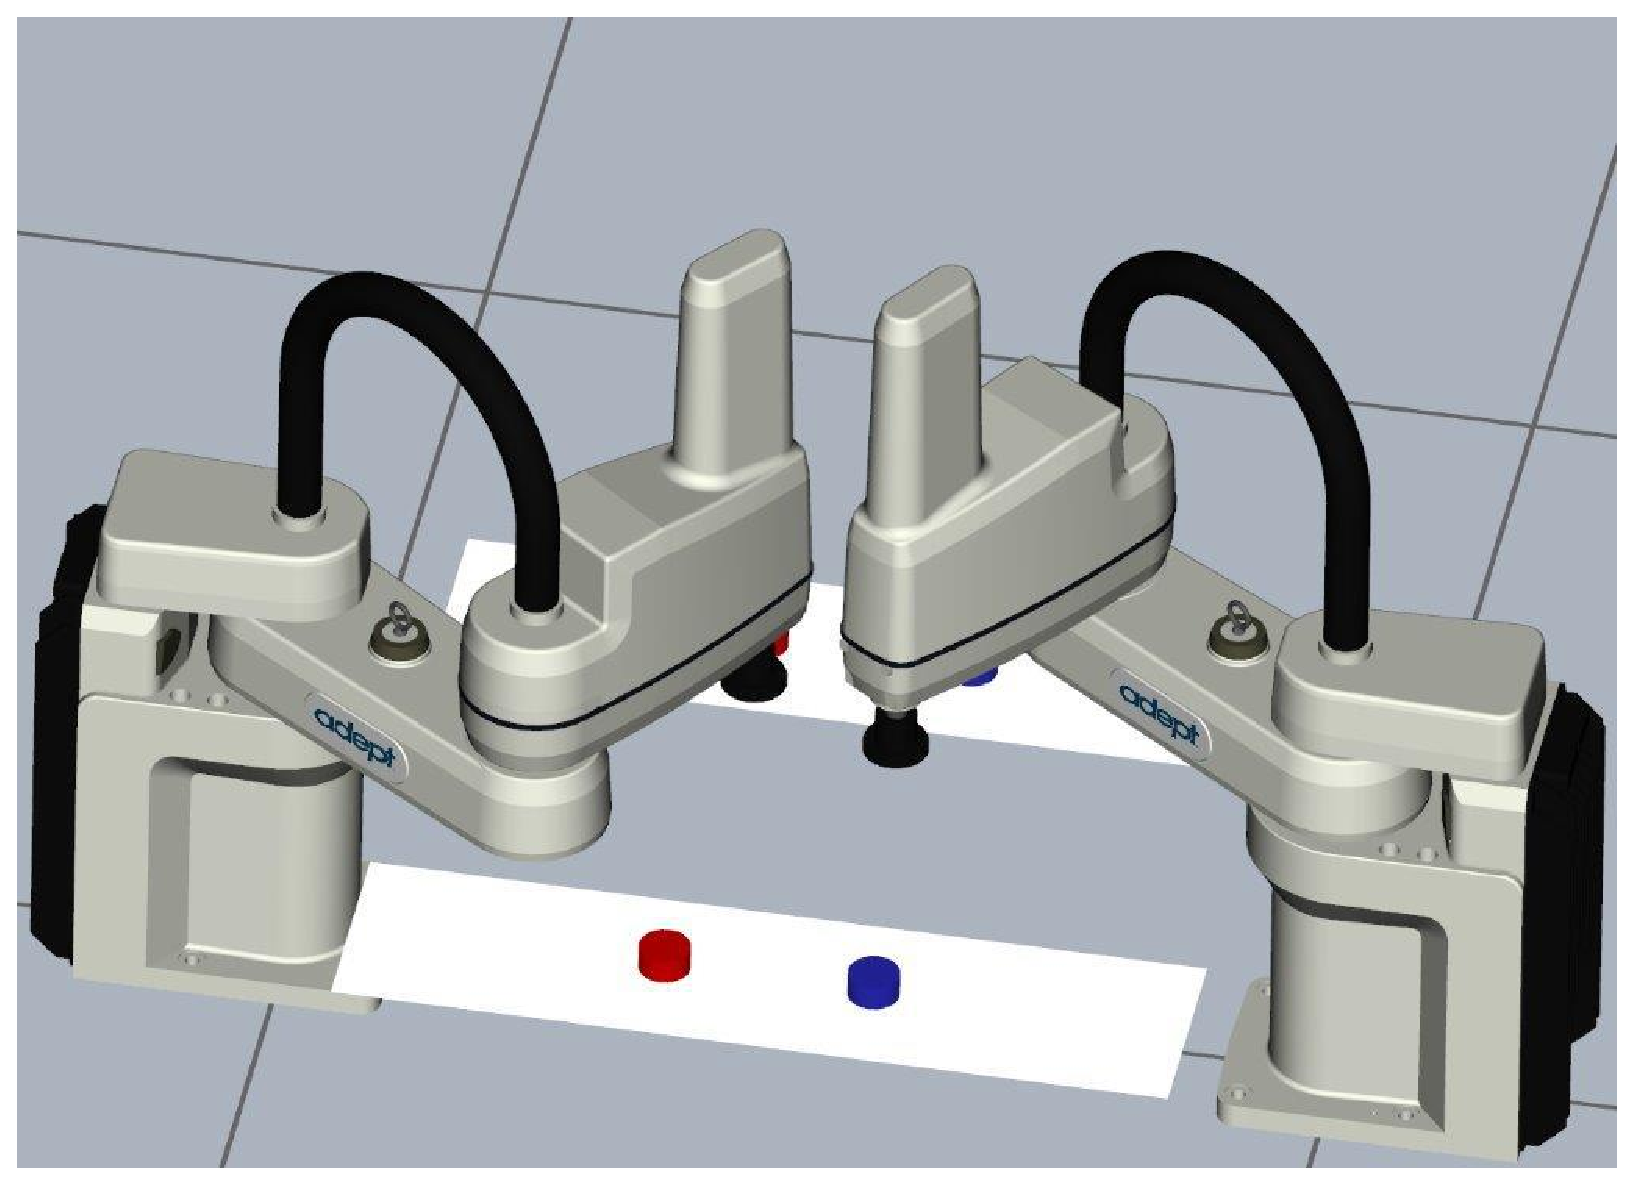
\includegraphics[scale=0.25]{cobra_3.eps}\\
            (3)
        }
    \end{minipage}
    \hfill
    \begin{minipage}[t]{0.49\textwidth}
        \centering{
            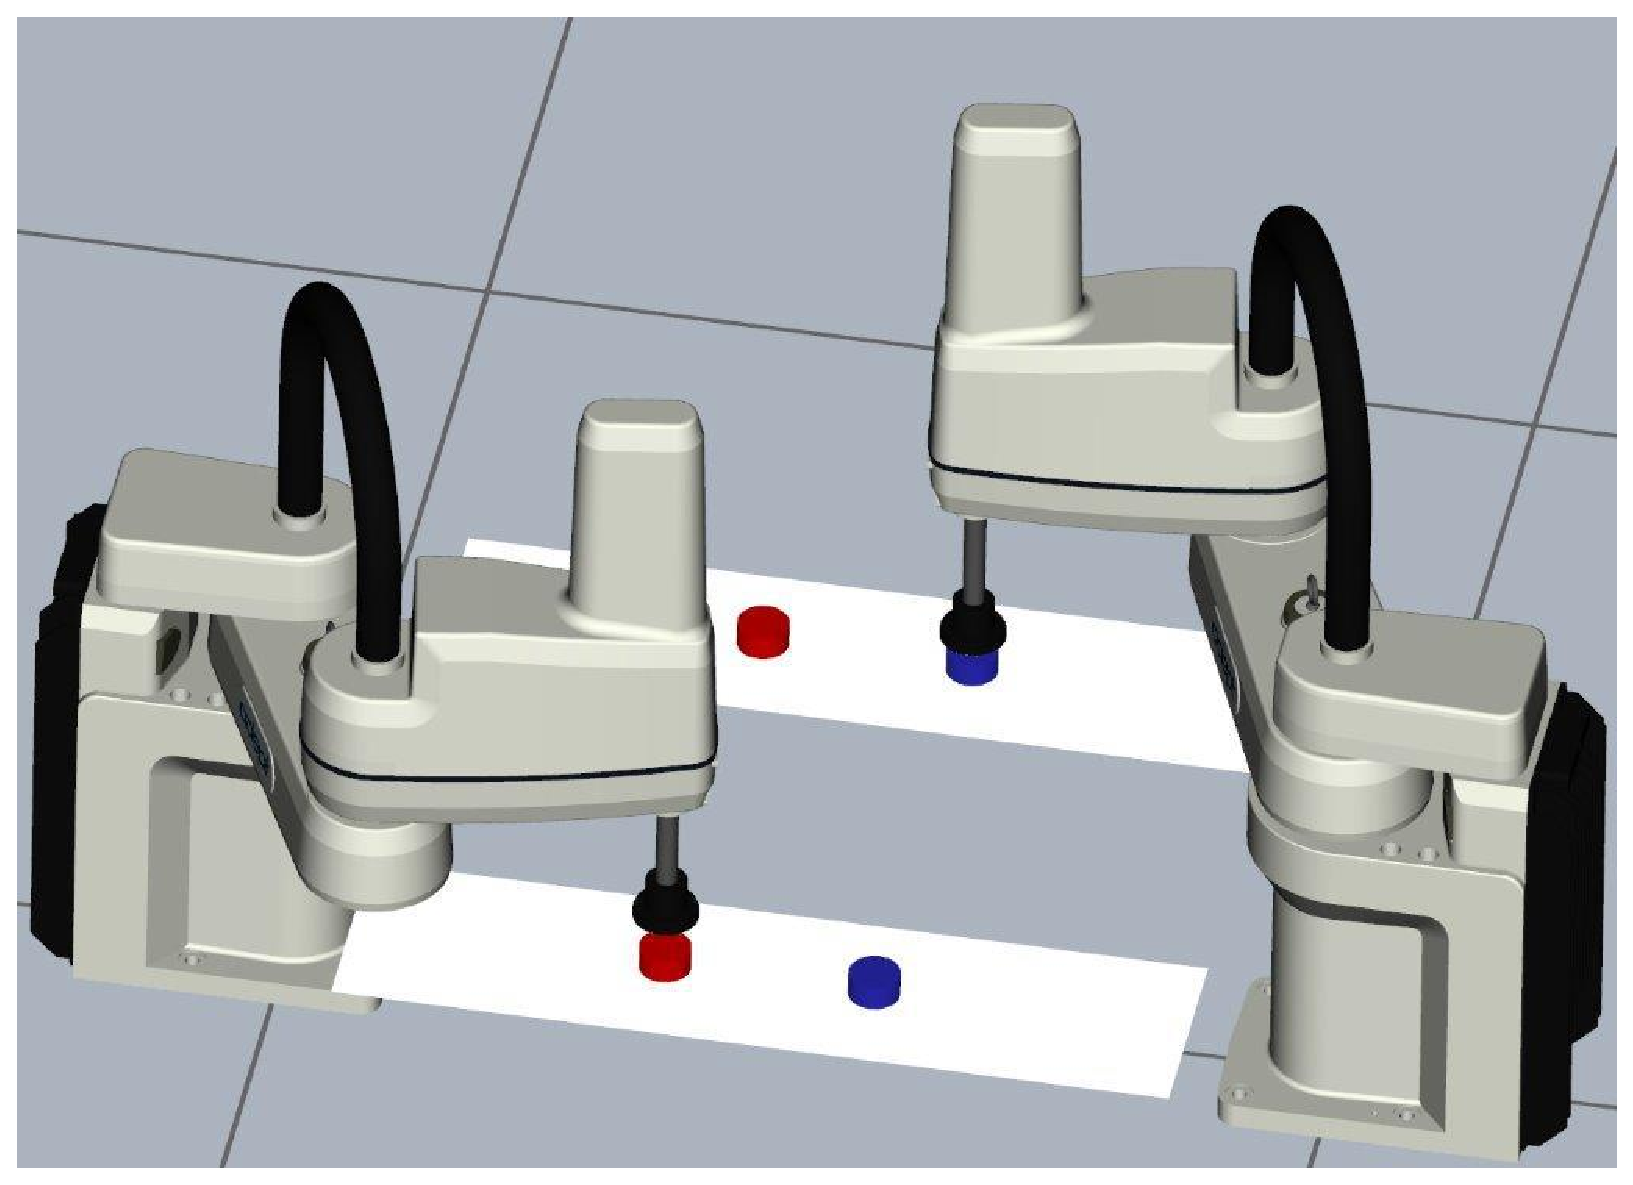
\includegraphics[scale=0.25]{cobra_4.eps}\\
            (4)
        }
    \end{minipage}
    \caption[Industrial manipulators in a shared environment.]{
        Two Adept Cobra \acs{SCARA} robots \cite{ADEPTsite} operating in a
        shared environment. The robots have to reach targets, indicated by
        colored cylinders, on two conveyors. A target for a particular robot
        may appear on either of the conveyors. In order to realize the tasks,
        the robots have to avoid collisions with each other.
    }
    \label{fig.cobra}
\end{figure}
%



%%%%%%%%%%%%%%%%%%%%%%%%%%%%%%%%%%%%%%%%%%%%%%%%%%%%%%%%%%%%%%%%%%%%%%%%%%%%%%%%
\subsection{Physical human-robot collaboration for carrying}\label{sec.robot_collaboration}

The execution of certain tasks may require physical collaboration of robots
with each other or with humans \cite{Caccavale2008handbook,
Bicchi2008handbook}. Humanoid robots are not an exception
\cite{Agravante2016preprint}. For example, they can assist humans in carrying
heavy or bulky objects, as shown in
\cref{fig.collaboration_box,fig.collaboration_stretcher}. The realization of
such collaboration was the goal of Joven Agravante during his Doctoral research
at LIRMM in Montpellier.


The transportation of an object requires walking and, hence, motion
anticipation, which must take into account two important aspects of physical
collaboration between the human and the robot:
%
\begin{itemize}
    \item it is necessary to account for the interaction forces exerted on the
        robot in order to maintain balance;

    \item it is necessary to react to human intentions conveyed through the
        interaction forces by adjusting motions of the robot appropriately, in
        particular, by adjusting its waking speed.
\end{itemize}
%
Joven addressed both of these aspects by developing the approximate
\nameref{model.CPPMJ} model, which incorporates the external wrench
$(\forceext, \momentext)$ acting on the \ac{CoM} of the robot. Thus, the
estimated interaction force applied to the \ac{CoM} is taken into account in
the balance preservation constraints and can influence the motion of the
\ac{CoM} through an impedance task of the following form
%
\begin{equation}
    \forceext^{xy}
    =
    \M{\Gamma}_{\V{x}}
    \V{x},
\end{equation}
%
where $\M{\Gamma}_{\V{x}}$ is an appropriately chosen matrix and the state of
the model is $\V{x} = (\C{c}^x, \dotC{c}^x, \ddotC{c}^x, \C{c}^y, \dotC{c}^y,
\ddotC{c}^y)$. The obtained model was employed in an \ac{MPC} scheme for
the generation of walking motions of an \sn{HRP-4} robot \cite{Kaneko2011iros}, as
illustrated in \cref{fig.collaboration_box,fig.collaboration_stretcher}. In
order to attain real-time performance of this scheme it was implemented by
Joven in \sn{C++} using the software framework \sn{HuMoTo}, which was designed and
partially implemented by the author. Experimental and theoretical results of
this work were reported in \cite{Agravante2016preprint, Agravante2016icra} and
Joven's thesis \cite{Agravante2015thesis}.


\begin{figure}[!htb]
    \begin{minipage}[t]{0.49\textwidth}
        \centering{
            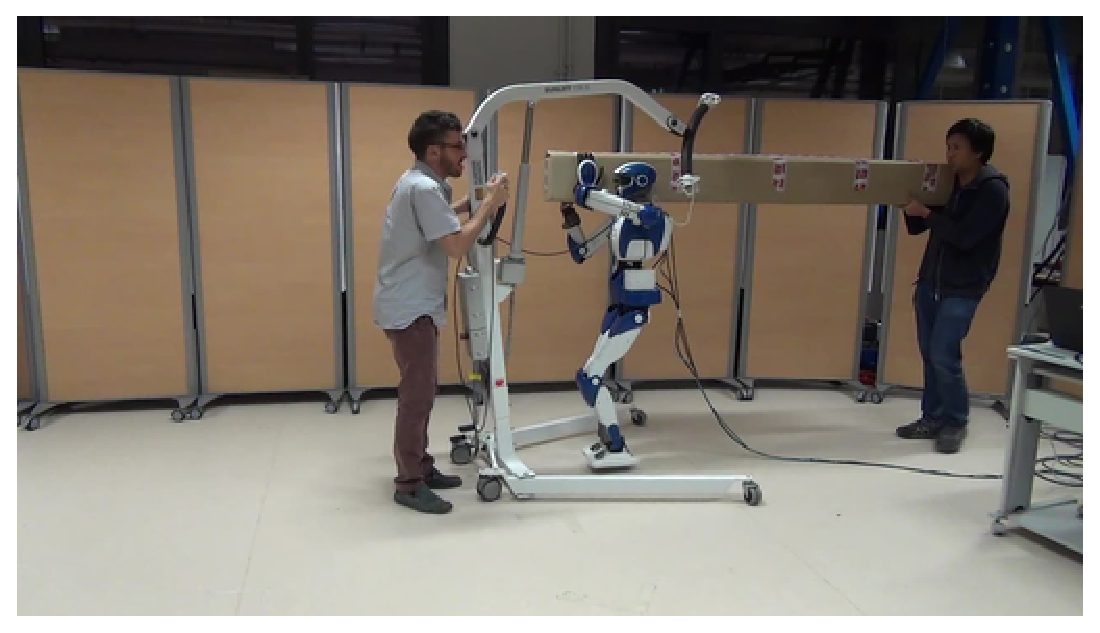
\includegraphics[scale=0.4]{collaboration_box2.eps}\\
            (1)
            \vspace{0.2cm}
        }
    \end{minipage}
    \hfill
    \begin{minipage}[t]{0.49\textwidth}
        \centering{
            \includegraphics[scale=0.4]{collaboration_box3.eps}\\
            (2)
            \vspace{0.2cm}
        }
    \end{minipage}
    \begin{minipage}[t]{0.49\textwidth}
        \centering{
            \includegraphics[scale=0.4]{collaboration_box4.eps}\\
            (3)
        }
    \end{minipage}
    \hfill
    \begin{minipage}[t]{0.49\textwidth}
        \centering{
            \includegraphics[scale=0.4]{collaboration_box5.eps}\\
            (4)
        }
    \end{minipage}
    \caption[Carrying a box in collaboration with a human.]{
        An \sn{HRP-4} \cite{Kaneko2011iros} carries a box in collaboration with
        a human.
    }
    \label{fig.collaboration_box}
\end{figure}


\begin{figure}[!htb]
    \begin{minipage}[t]{0.49\textwidth}
        \centering{
            \includegraphics[scale=0.4]{collaboration_stretcher1.eps}\\
            (1)
            \vspace{0.2cm}
        }
    \end{minipage}
    \hfill
    \begin{minipage}[t]{0.49\textwidth}
        \centering{
            \includegraphics[scale=0.4]{collaboration_stretcher3.eps}\\
            (2)
            \vspace{0.2cm}
        }
    \end{minipage}
    \begin{minipage}[t]{0.49\textwidth}
        \centering{
            \includegraphics[scale=0.4]{collaboration_stretcher5.eps}\\
            (3)
        }
    \end{minipage}
    \hfill
    \begin{minipage}[t]{0.49\textwidth}
        \centering{
            \includegraphics[scale=0.4]{collaboration_stretcher7.eps}\\
            (4)
        }
    \end{minipage}
    \caption[Carrying a stretcher in collaboration with a human.]{
        An \sn{HRP-4} \cite{Kaneko2011iros} carries a stretcher in
        collaboration with a human.
    }
    \label{fig.collaboration_stretcher}
\end{figure}
